\documentclass[11pt, oneside]{article}   	% use "amsart" instead of "article" for AMSLaTeX format

\usepackage{geometry}                		% See geometry.pdf to learn the layout options. There are lots.
\geometry{letterpaper}                   		% ... or a4paper or a5paper or ... 
% \geometry{landscape}                		% Activate for for rotated page geometry
% \usepackage[parfill]{parskip}    		% Activate to begin paragraphs with an empty line rather than an indent
\usepackage{graphicx}				% Use pdf, png, jpg, or eps§ with pdflatex; use eps in DVI mode
% TeX will automatically convert eps --> pdf in pdflatex		
\usepackage{amssymb}
\usepackage[table]{xcolor}
\usepackage{array}
\usepackage{xspace}
\usepackage{accents}

\newcommand{\PQb}{\ensuremath{\mathrm{b}}\xspace} % b
\newcommand{\PAQb}{\ensuremath{\overline{\mathrm{b}}}\xspace} %
\newcommand{\bbbar}{\ensuremath{\PQb\PAQb}\xspace}
\newcommand{\PQq}{\ensuremath{\mathrm{q}}\xspace} % quark (generic)
\newcommand{\PAQq}{\ensuremath{\overline{\mathrm{q}}}\xspace} % quark (generic)
\newcommand{\qqbar}{\ensuremath{\PQq\PAQq}\xspace}
\newcommand{\ttbar}{\ensuremath{\mathrm{t}\overline{\mathrm{t}}}\xspace} % t-tbar
 \newcommand{\Pp}{\ensuremath{{p}}}
\providecommand{\PSg}{\ensuremath{\widetilde{\mathrm{g}}}\xspace} % gluino
 \newcommand{\njets}{N_{\rm jet}}
  \newcommand{\nbjets}{N_{\rm b-jet}}
\newcommand{\PSGczDo}{\ensuremath{\widetilde{\chi}^{0}_{1}}\xspace} % neutralino
\newcommand{\MHT}{H_{\mathrm T}^{\rm miss}}
\newcommand{\HT}{H_{\mathrm T}}
\newcommand{\GeV}{\ensuremath{\,\text{Ge\hspace{-.08em}V}}\xspace}

\title{Auxiliary material for CERN-EP-2016-036}
\author{RA2/b Team}
% \date{}							% Activate to display a given date or no date

\begin{document}
\maketitle

\begin{figure}[htb]
  \centering
  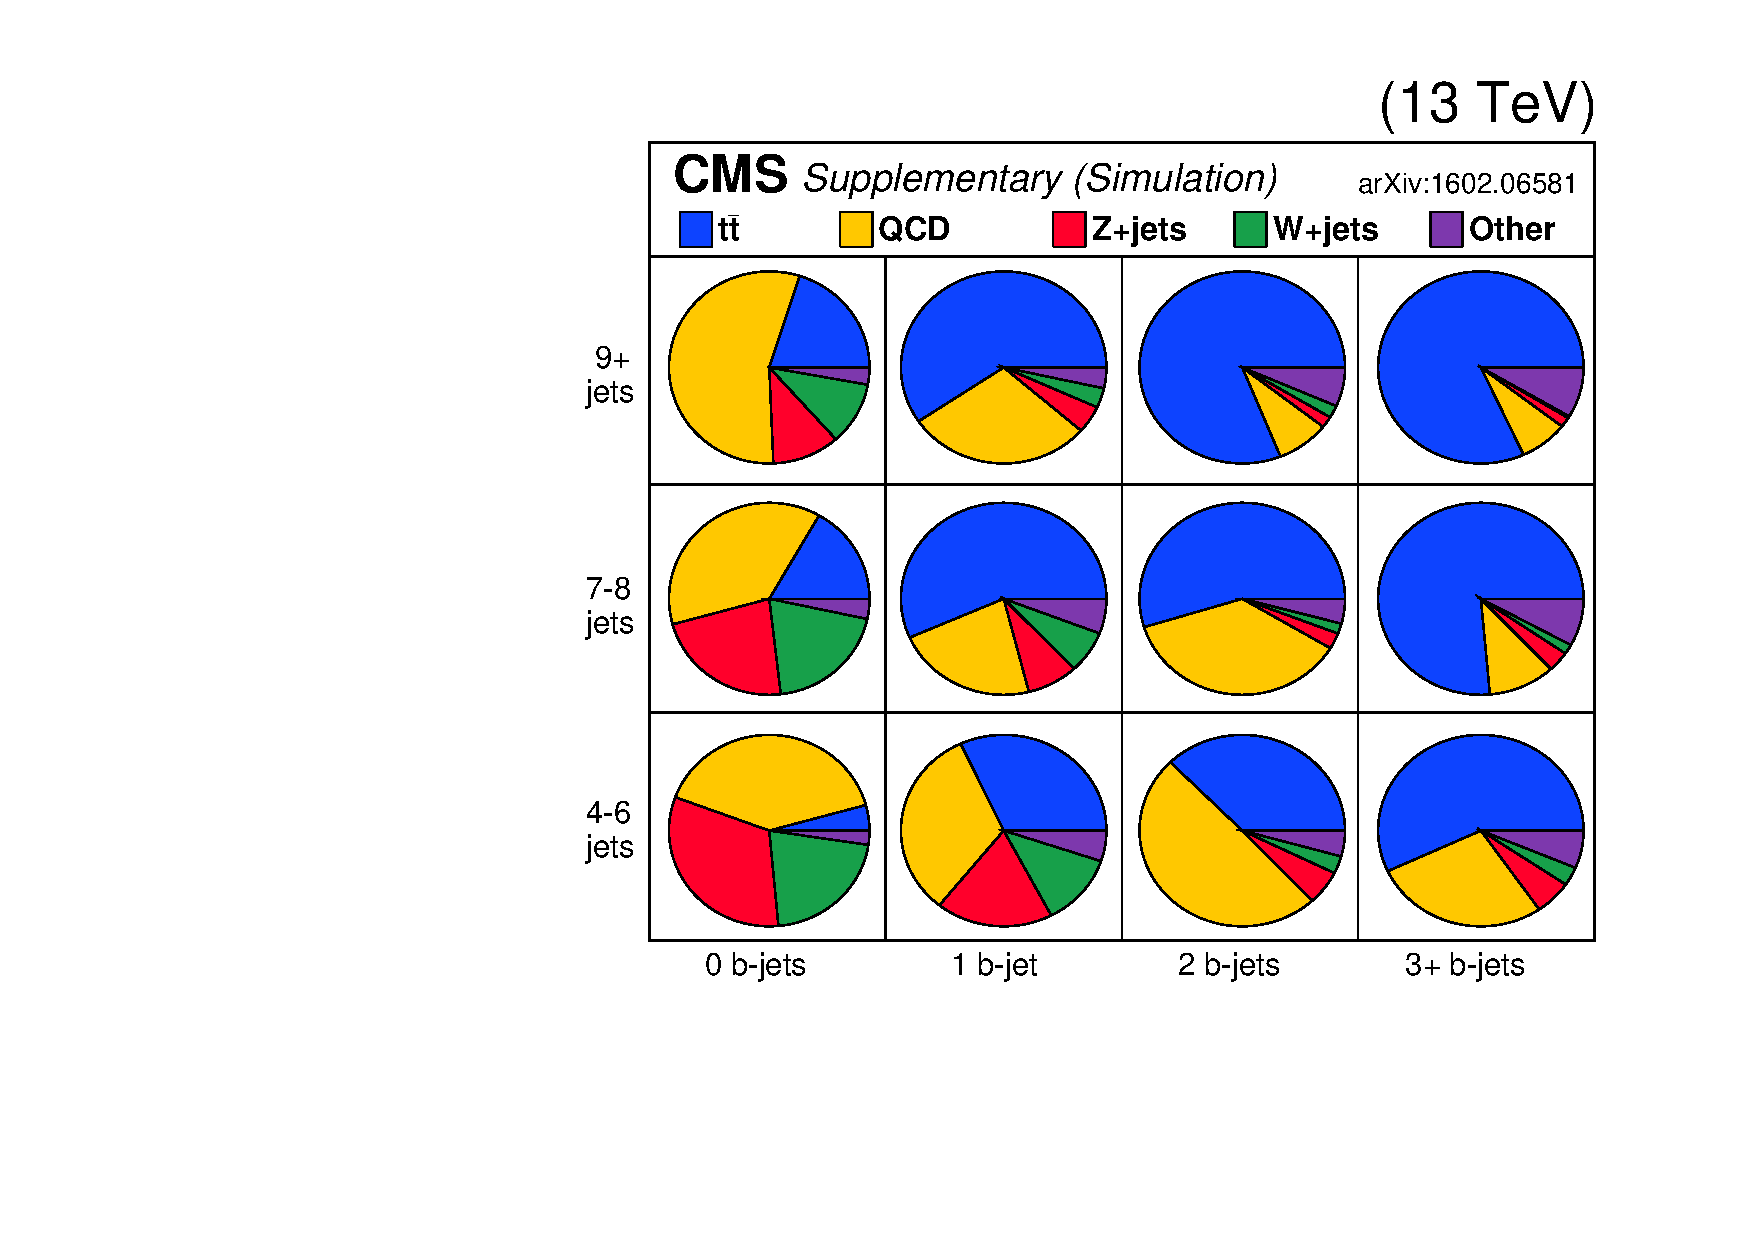
\includegraphics[width=0.9\textwidth]{MC_BG_Pie_vs_NJets_NBJets.pdf}
  \caption{
    Background composition in zero-lepton search region ($H_{\rm T}^{\mathrm{miss}}>200$ GeV, $H_{\rm T}>500$ GeV) in bins of the number of jets and the number of b-tagged jets. The expected contribution from each process is obtained from simulation after applying the full baseline selection. 
  }
\end{figure}

\begin{figure}[htb]
  \centering
  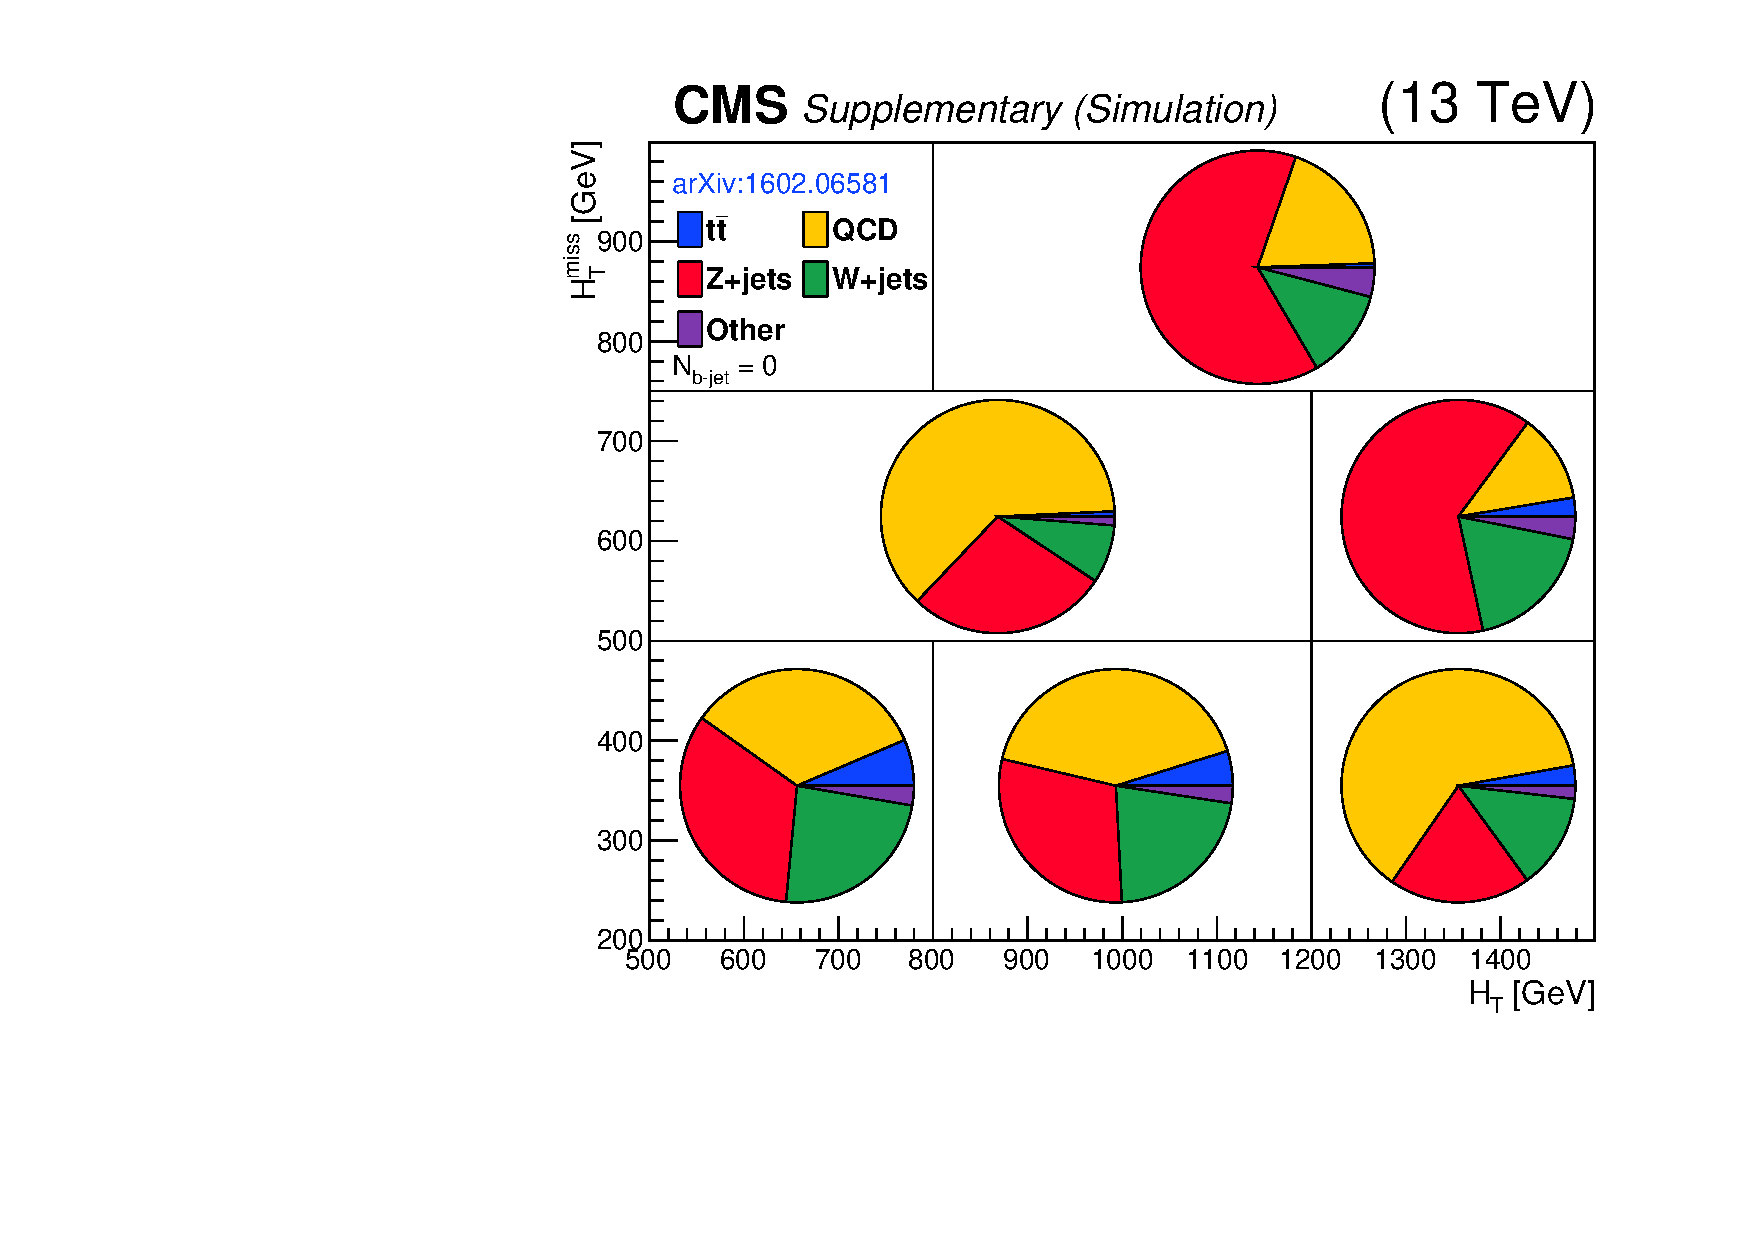
\includegraphics[width=0.48\textwidth]{MC_BG_Pie_NB0.pdf}
  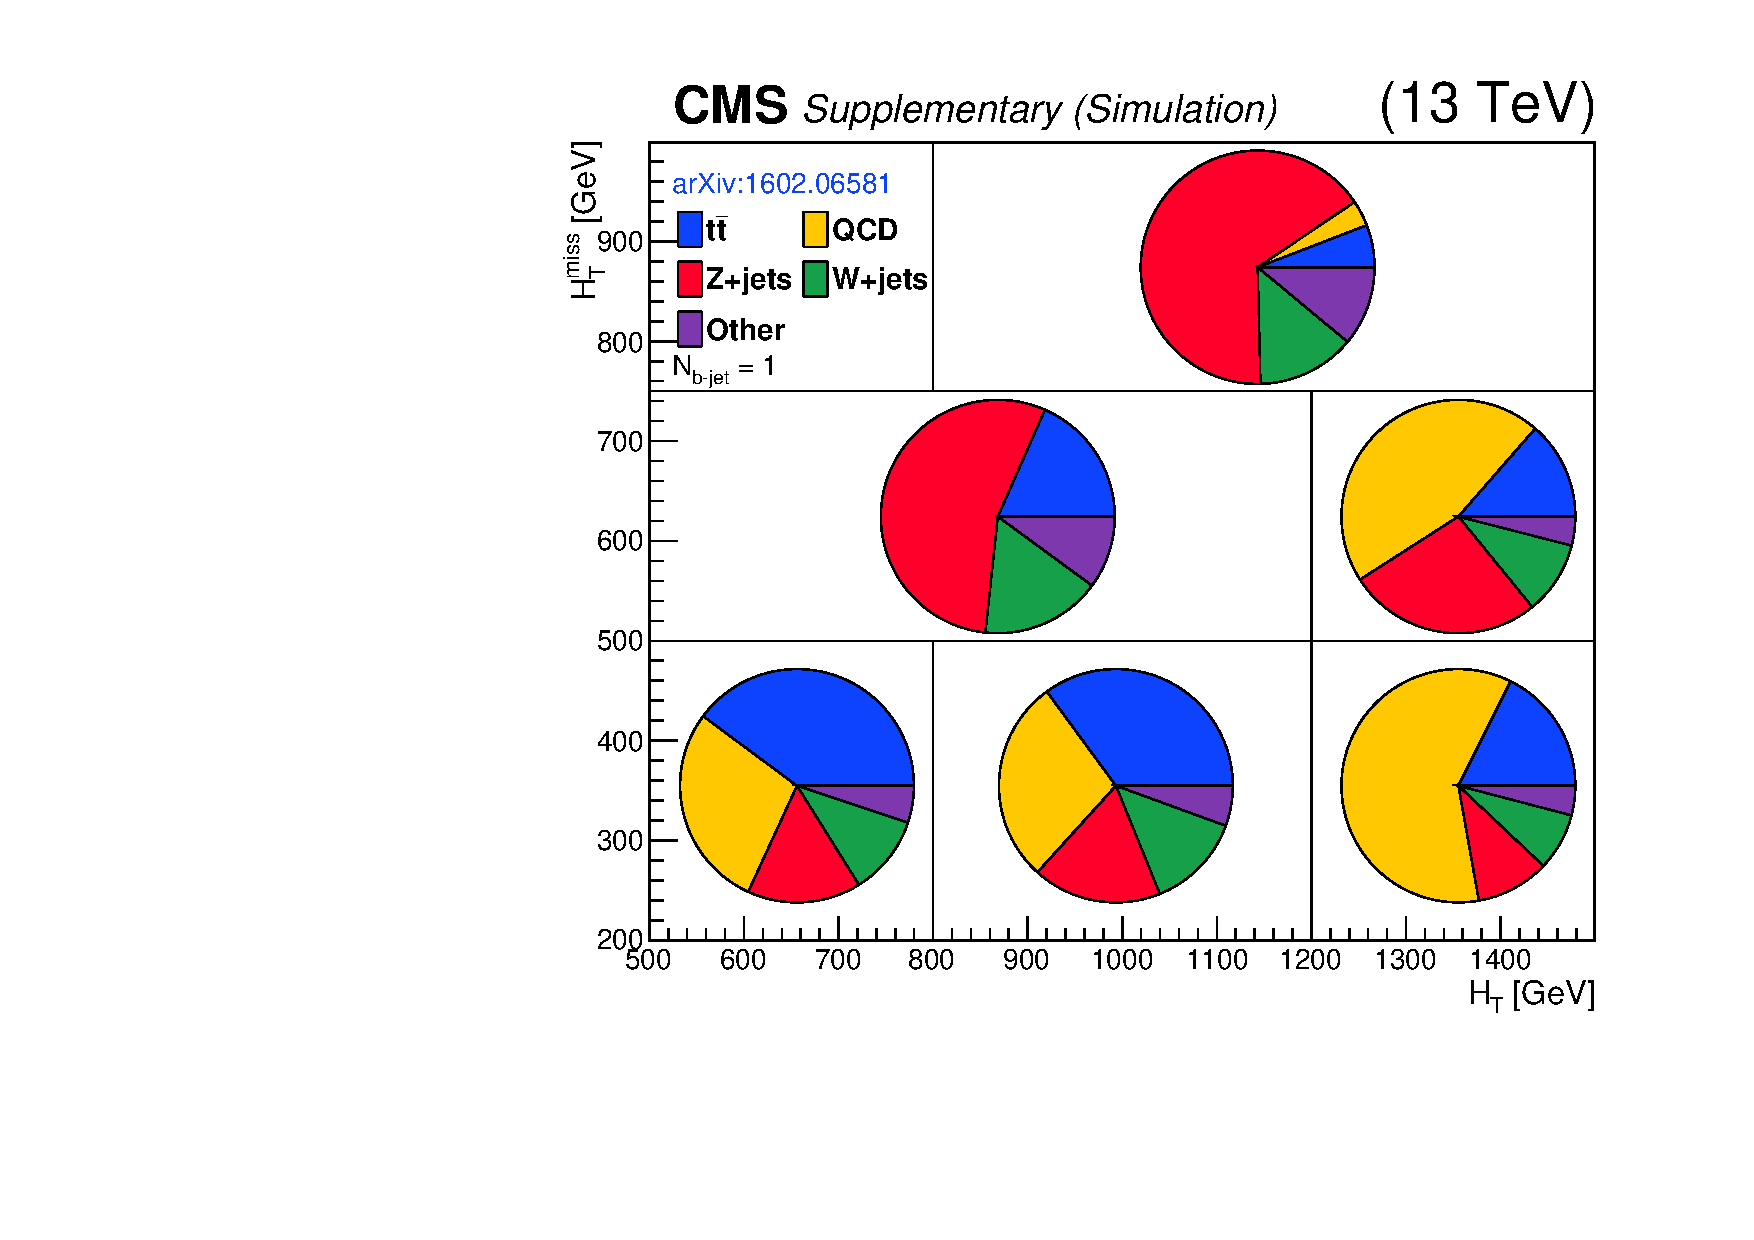
\includegraphics[width=0.48\textwidth]{MC_BG_Pie_NB1.pdf} \\
   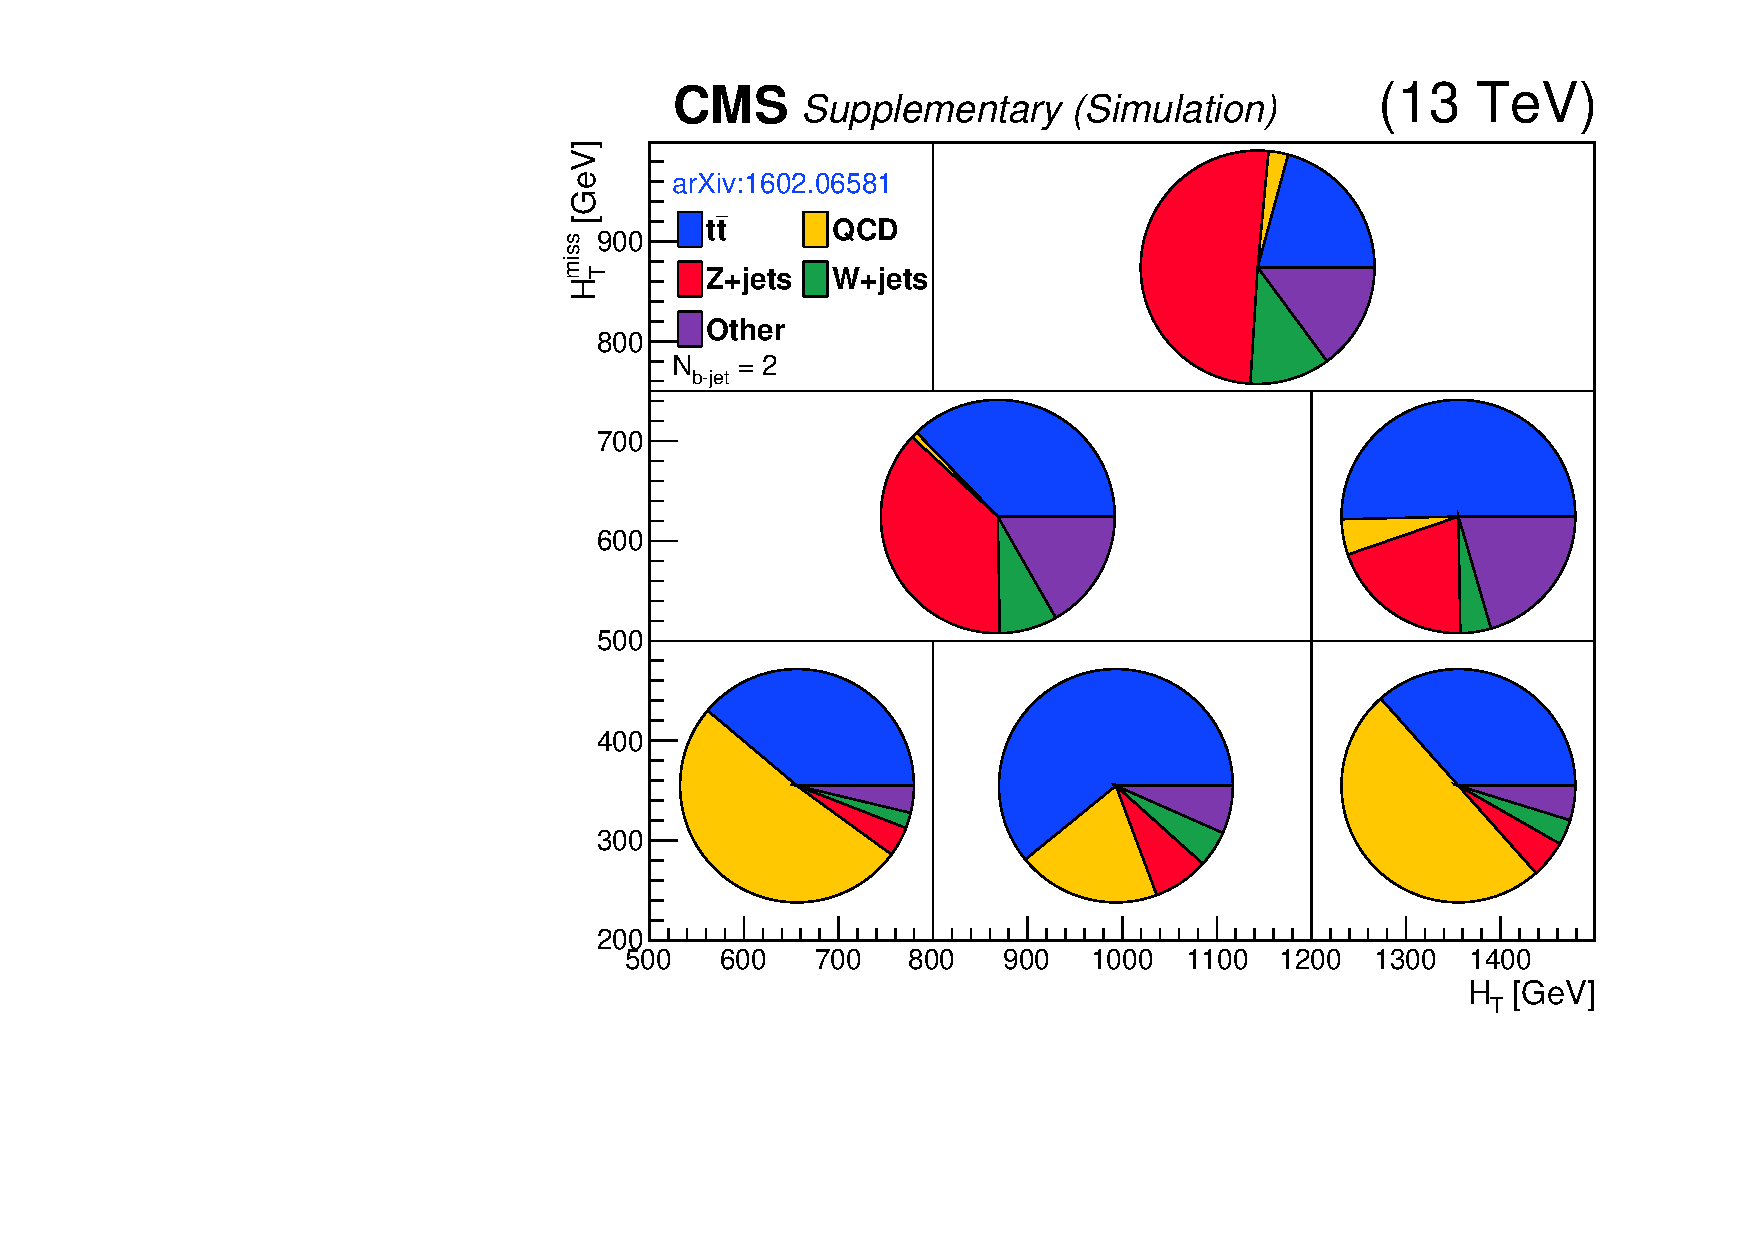
\includegraphics[width=0.48\textwidth]{MC_BG_Pie_NB2.pdf}
  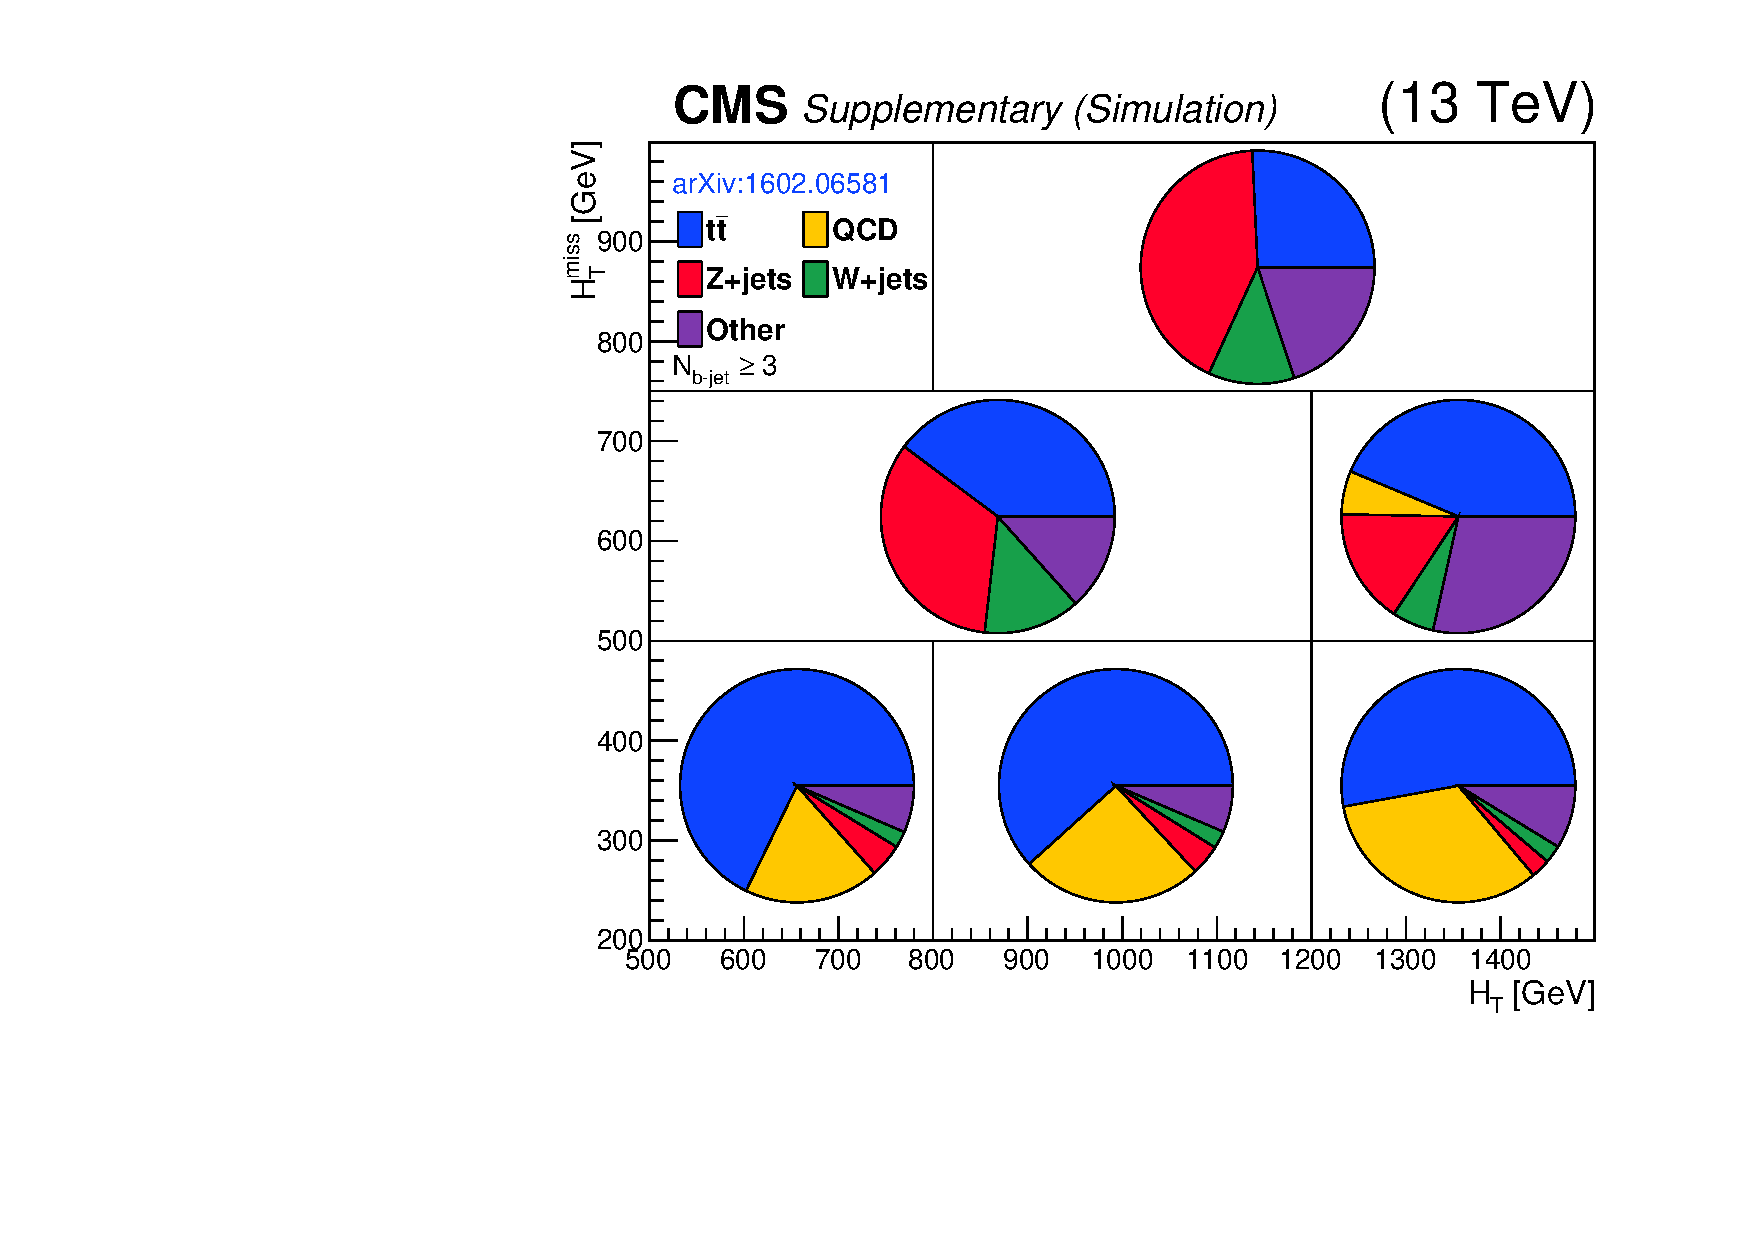
\includegraphics[width=0.48\textwidth]{MC_BG_Pie_NB3.pdf}
  \caption{
    Background composition from simulation in zero-lepton search region in bins of $H_{\rm T}^{\mathrm{miss}}$ and $H_{\rm T}$. The composition is shown separately for events with (top-left) 0 b-tagged jets, (top-right) 1 b-tagged jet, (bottom-left) 2 b-tagged jets, and (bottom-left) at least 3 b-tagged jets.
    }
\end{figure}

\begin{figure}[htb]
  \centering
  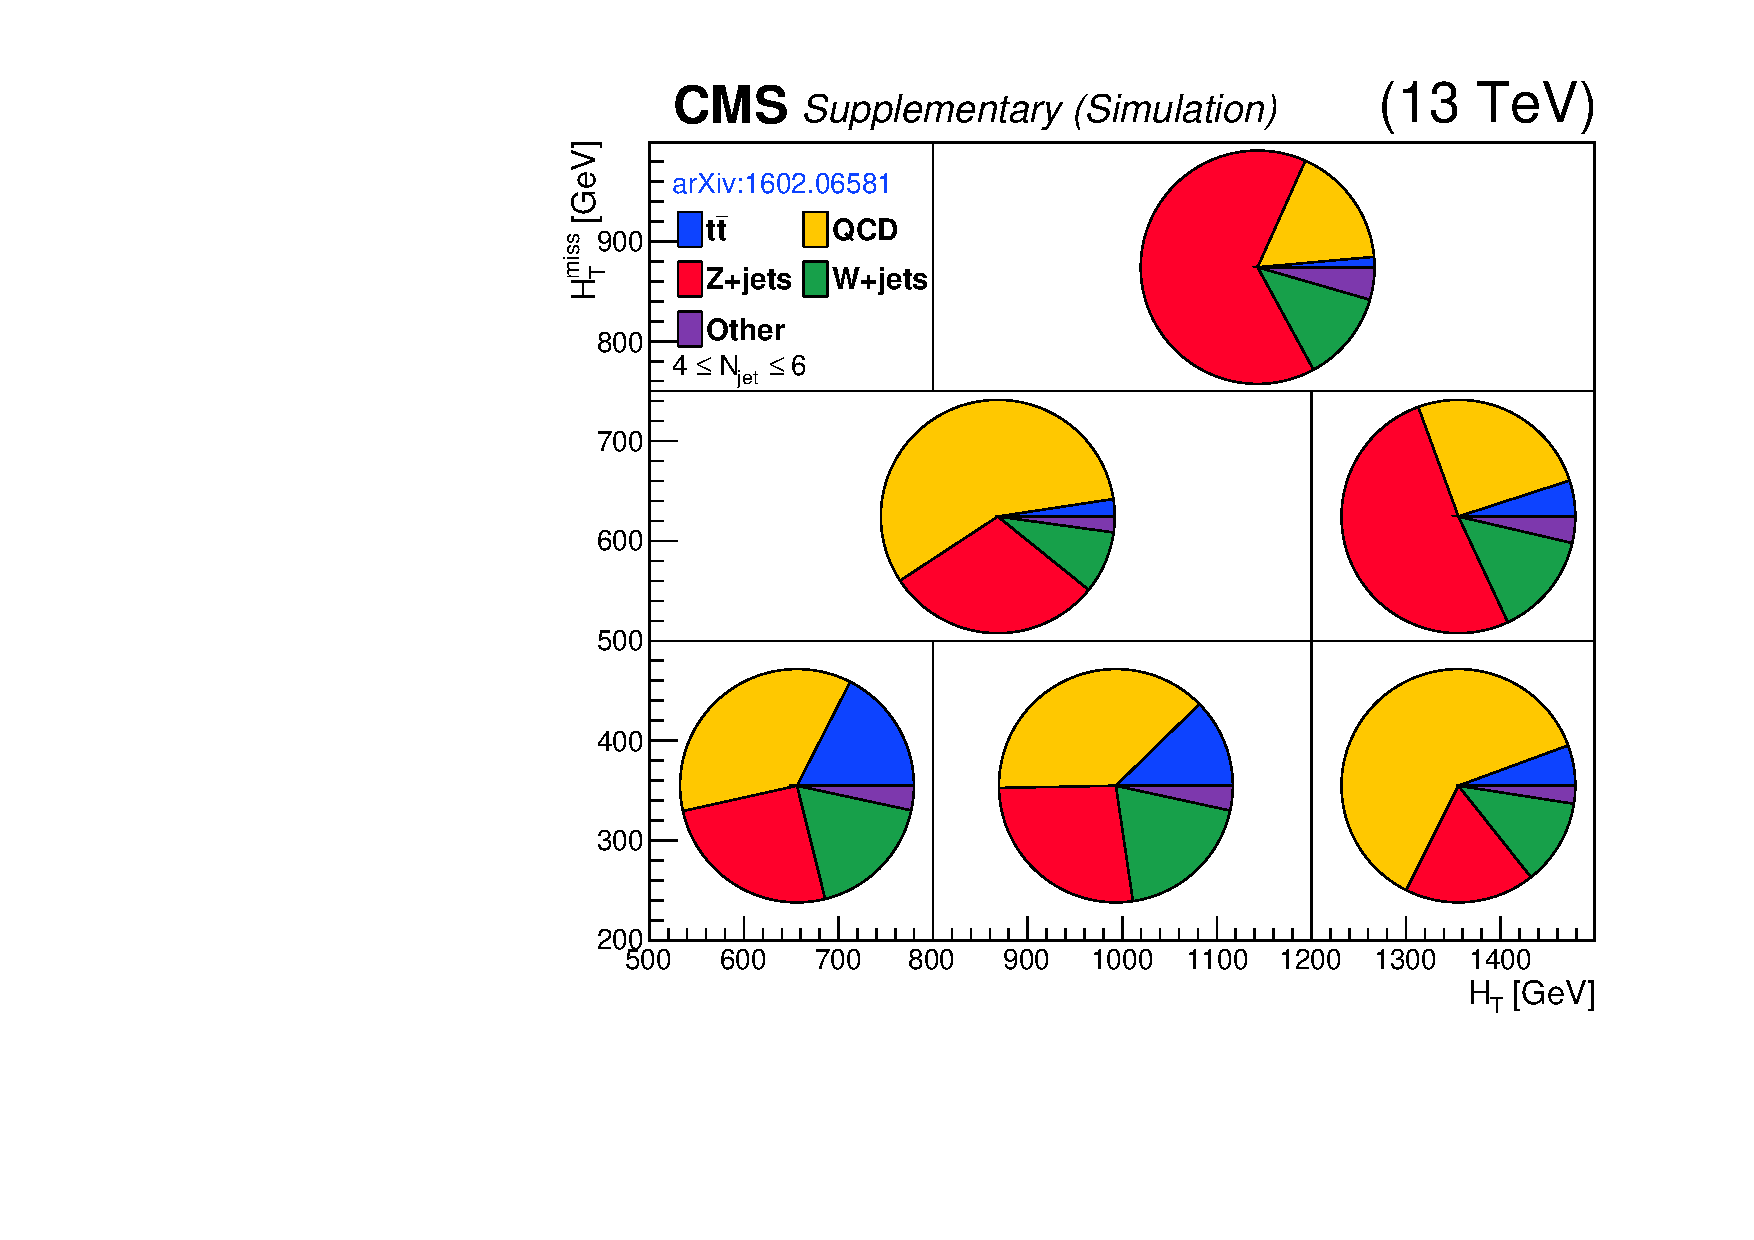
\includegraphics[width=0.48\textwidth]{MC_BG_Pie_NJ4-6.pdf}
  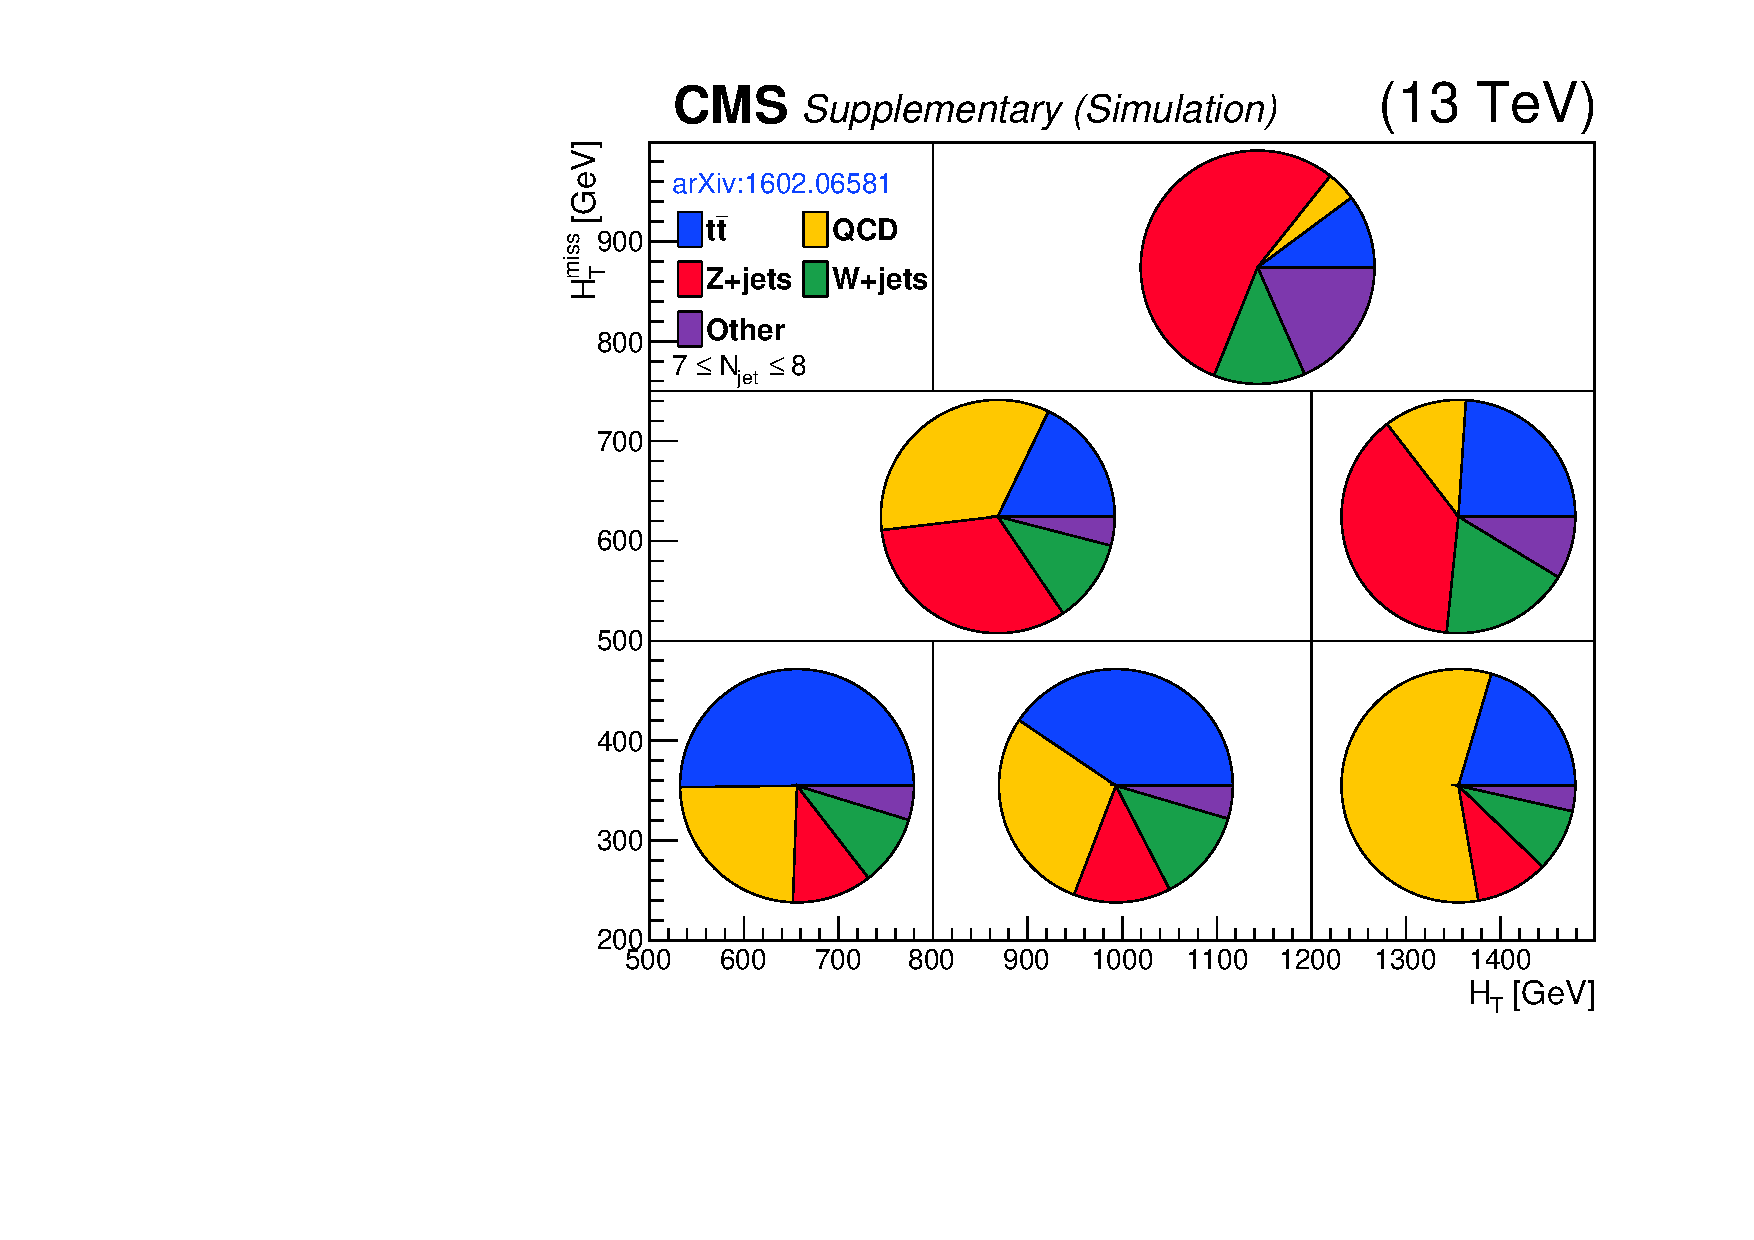
\includegraphics[width=0.48\textwidth]{MC_BG_Pie_NJ7-8.pdf} \\
   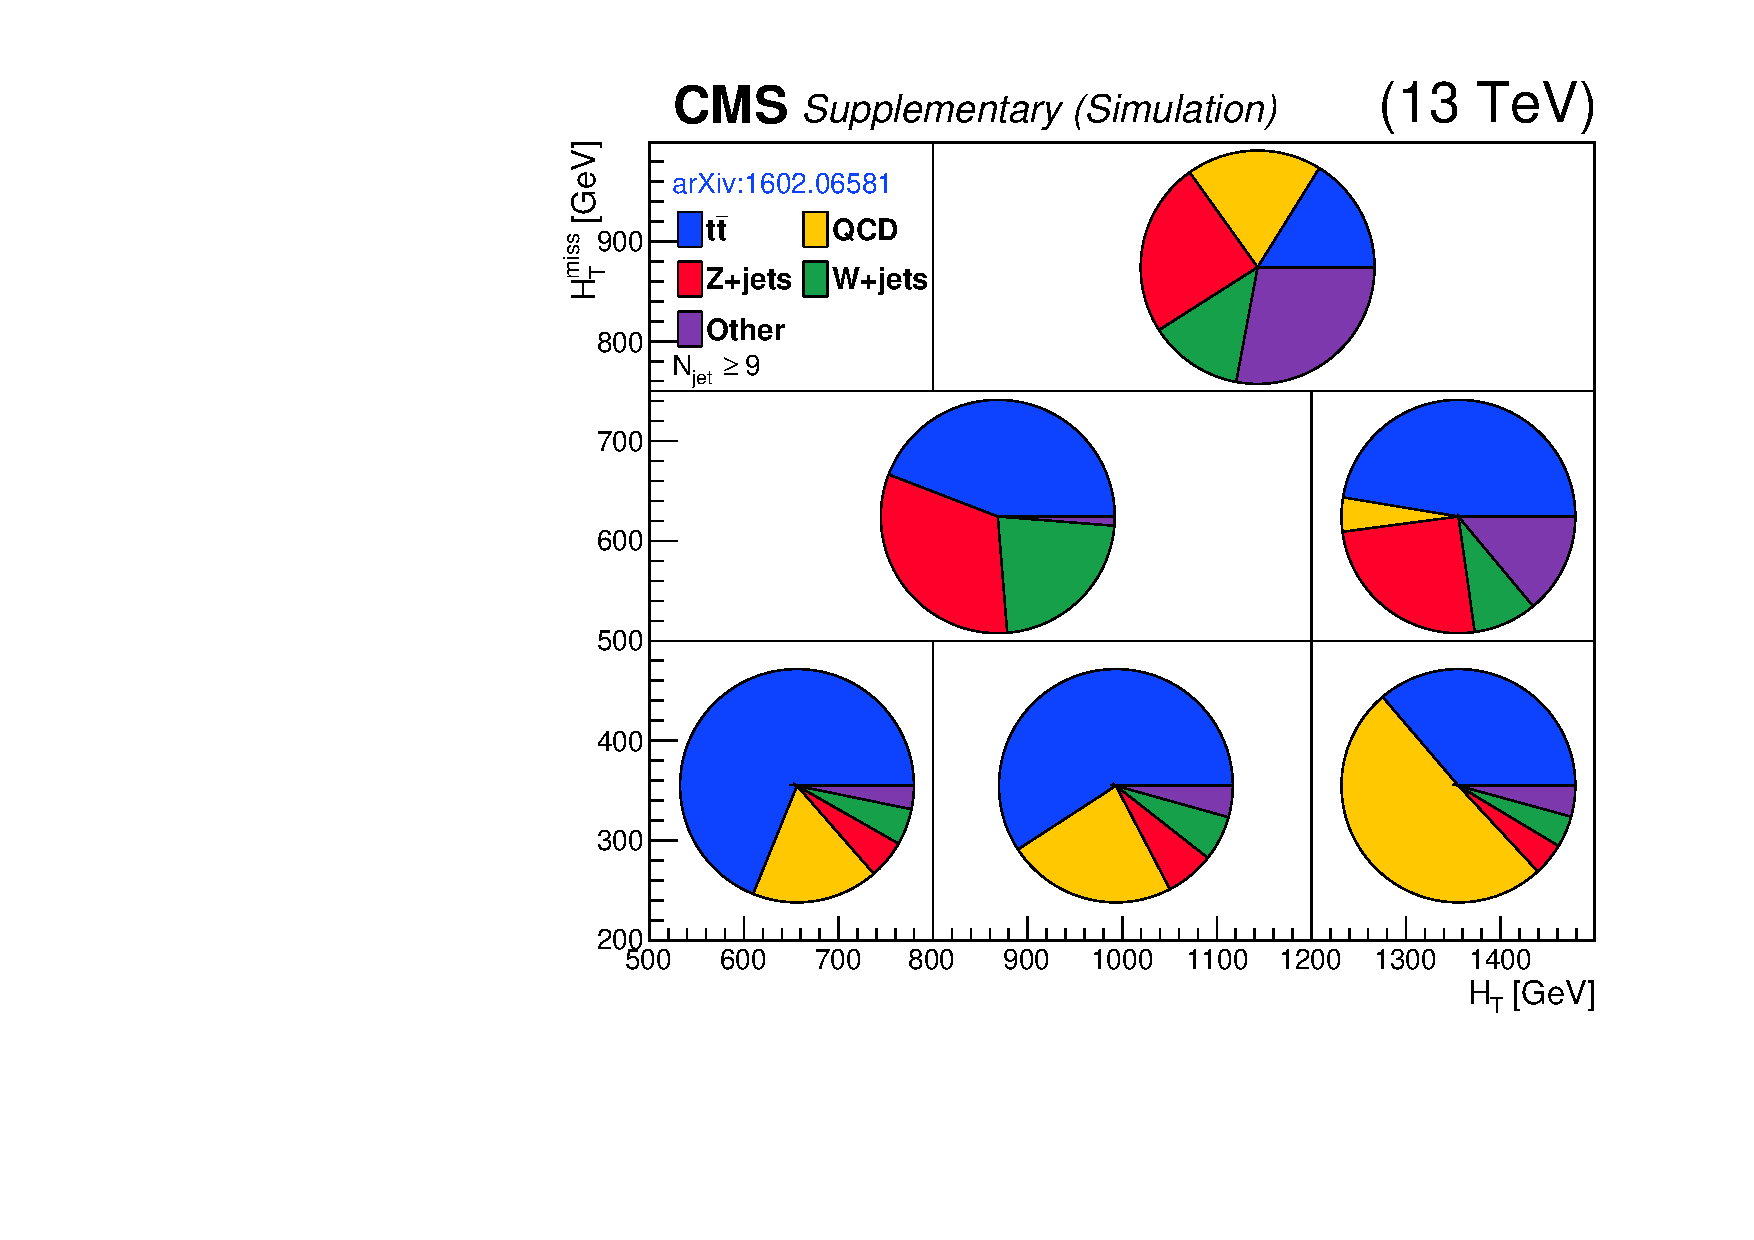
\includegraphics[width=0.48\textwidth]{MC_BG_Pie_NJ9.pdf}
  \caption{
    Background composition from simulation in zero-lepton search region in bins of $H_{\rm T}^{\mathrm{miss}}$ and $H_{\rm T}$. The composition is shown separately for events with (left) 4-6 jets, (middle) 7-8 jets, and (right) at least 9 jets.
     	   }
\end{figure}

\begin{figure}[htb]
  \centering
  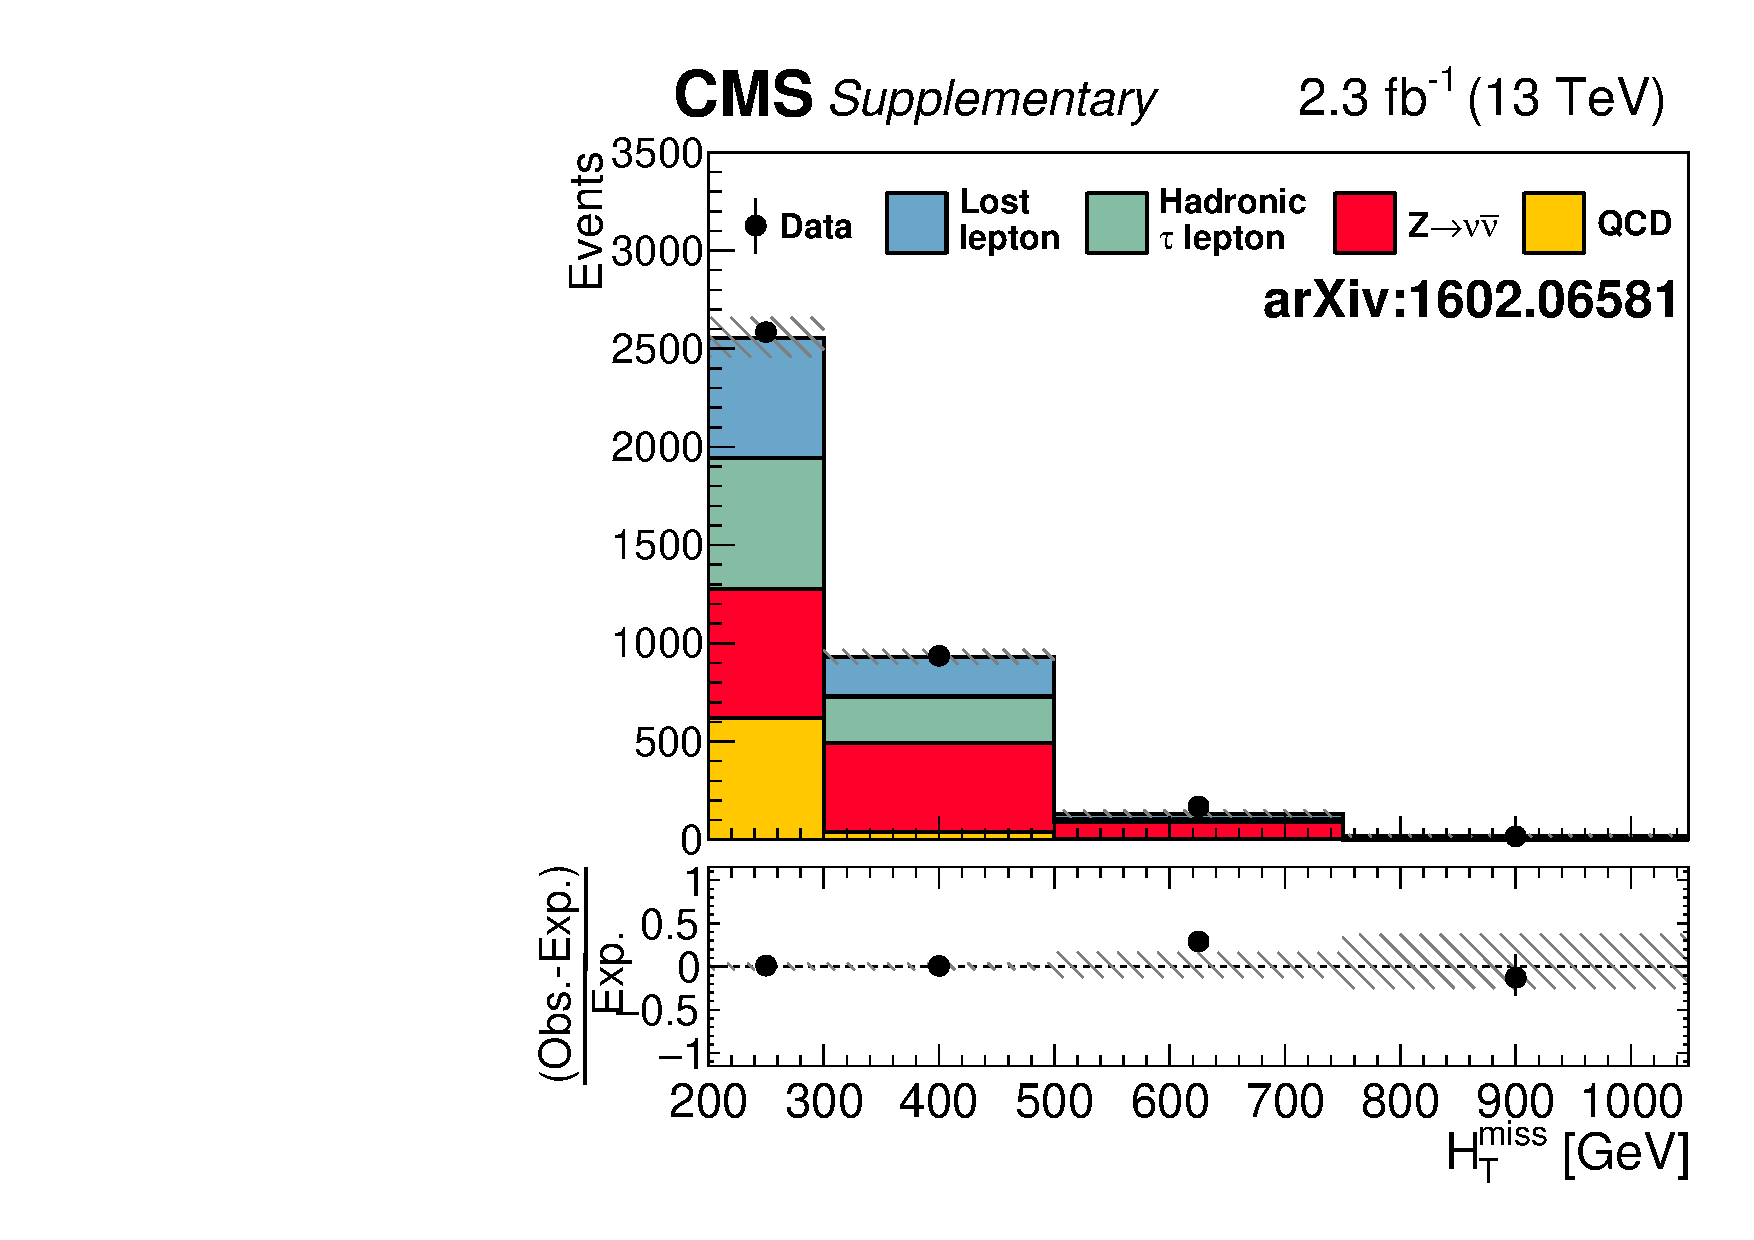
\includegraphics[width=0.48\textwidth]{1D-projection-allMHT.pdf}
  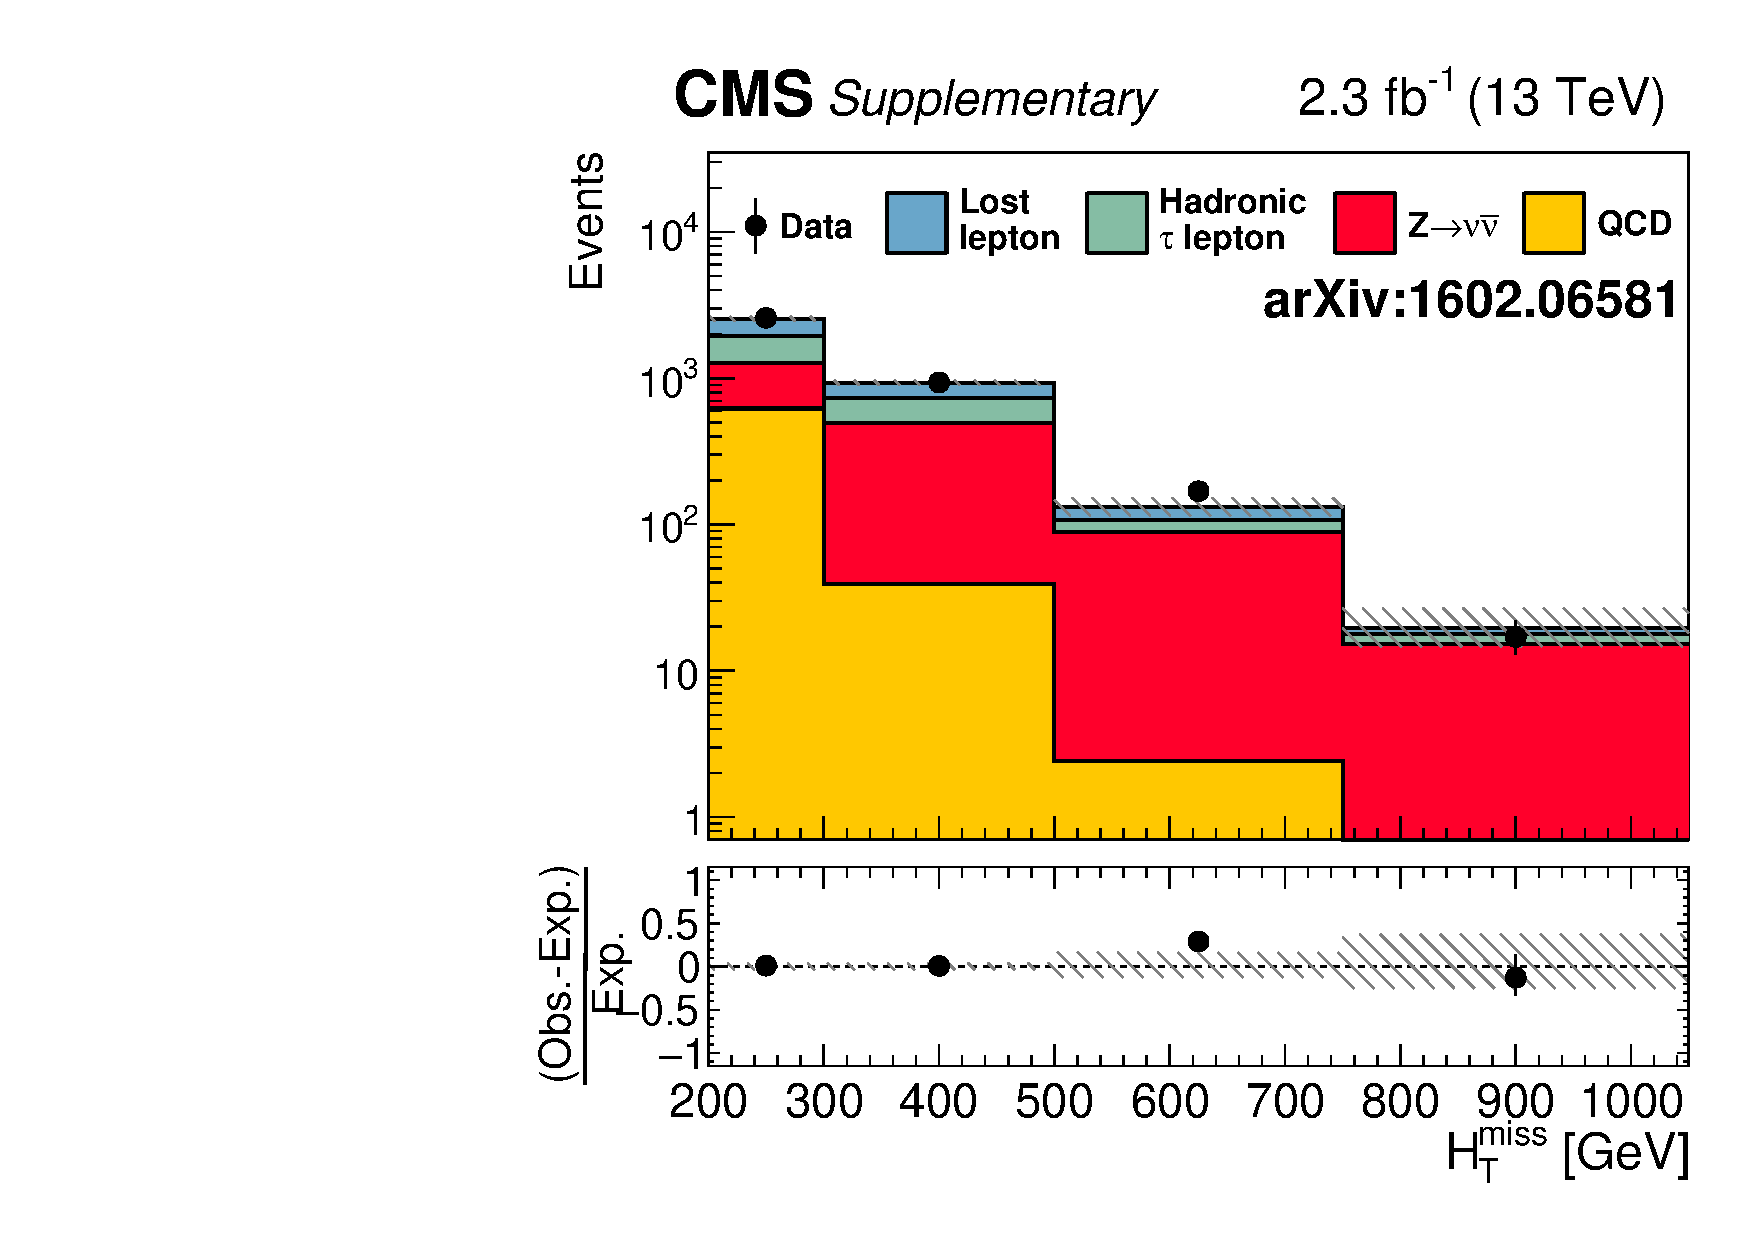
\includegraphics[width=0.48\textwidth]{1D-projection-allMHT-log.pdf}
  \caption{
    The distributions of observed number of events and predicted background as a function of $H_{\rm T}^{\rm miss}$, plotted on linear (left) and log (right) scales. Distributions are integrated over other binned observables in the analysis, number of b-tagged jets, number of jets, and $H_{\rm T}$. 
  }
\end{figure}

\begin{figure}[htb]
  \centering
  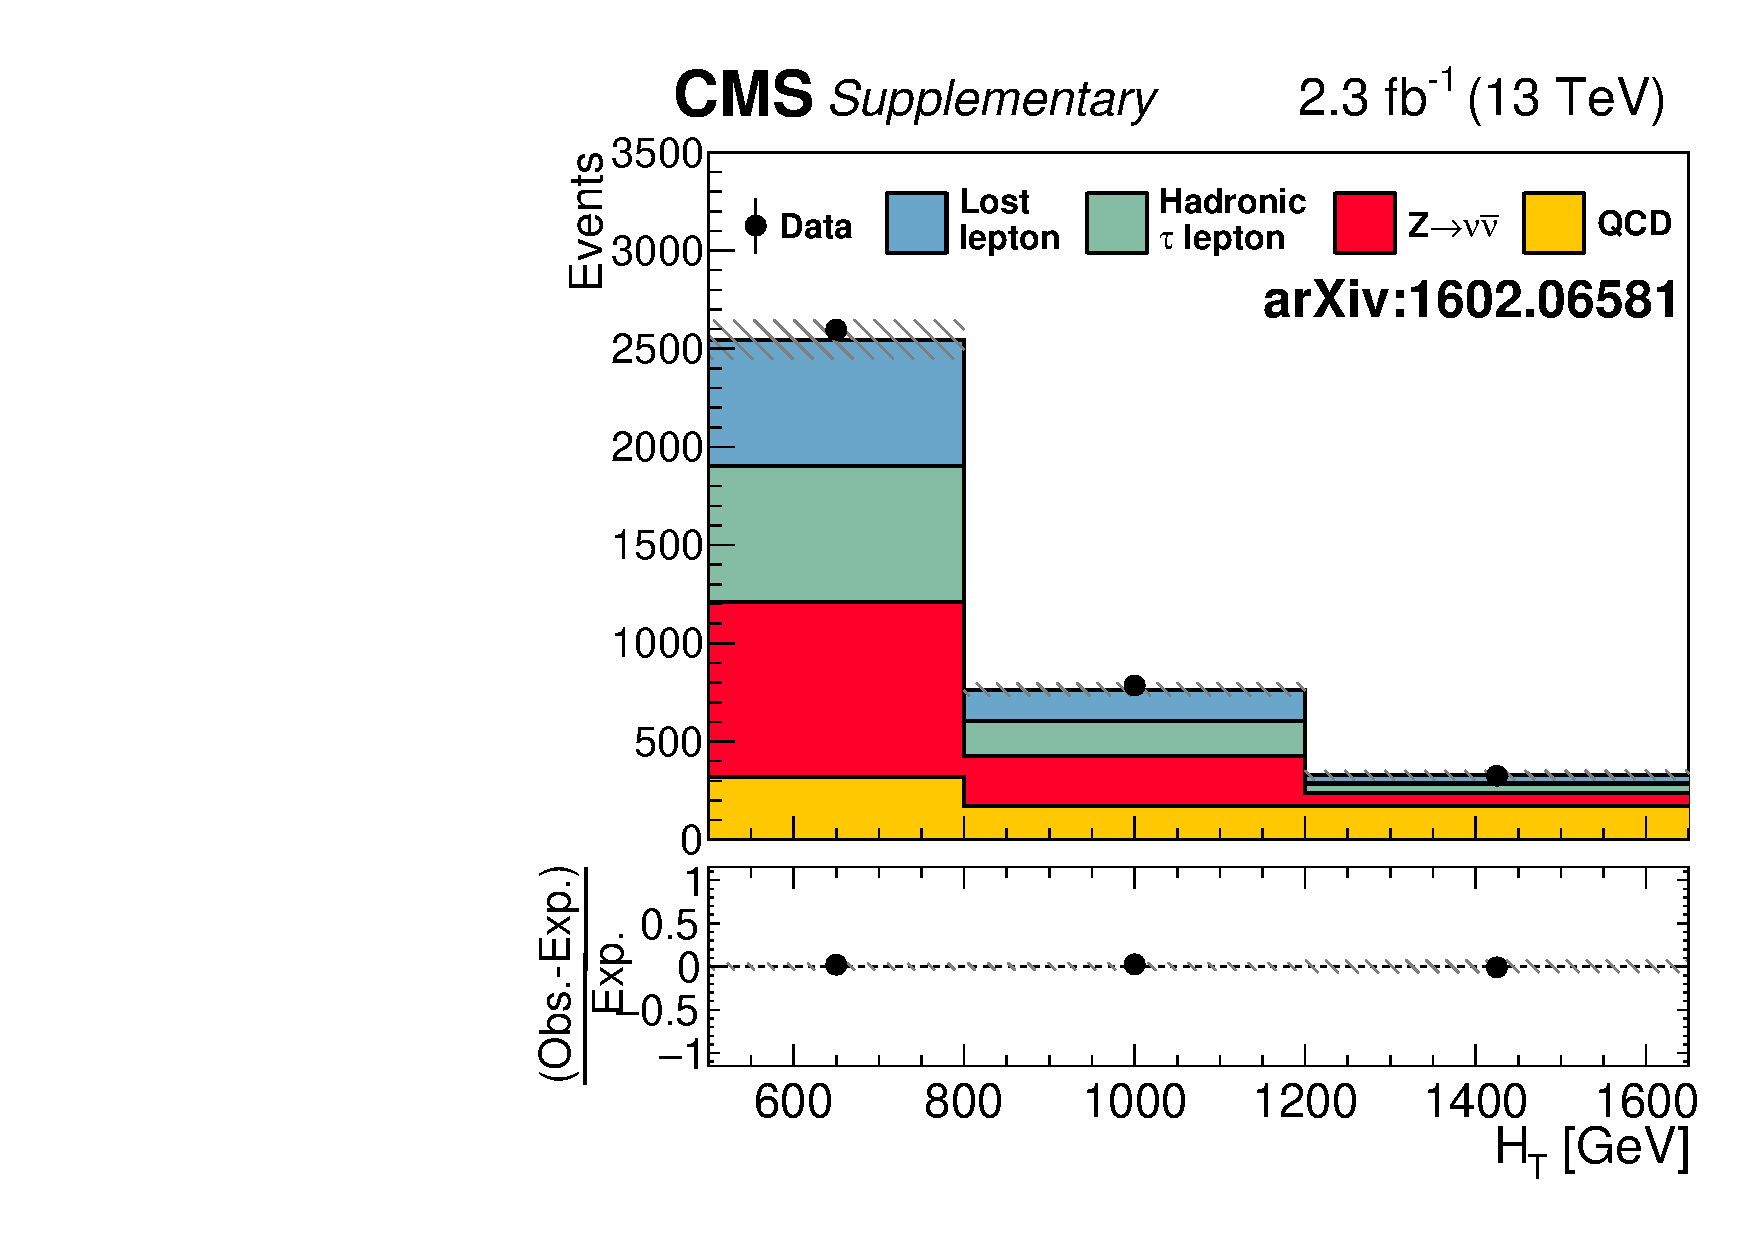
\includegraphics[width=0.48\textwidth]{1D-projection-allHT.pdf}
  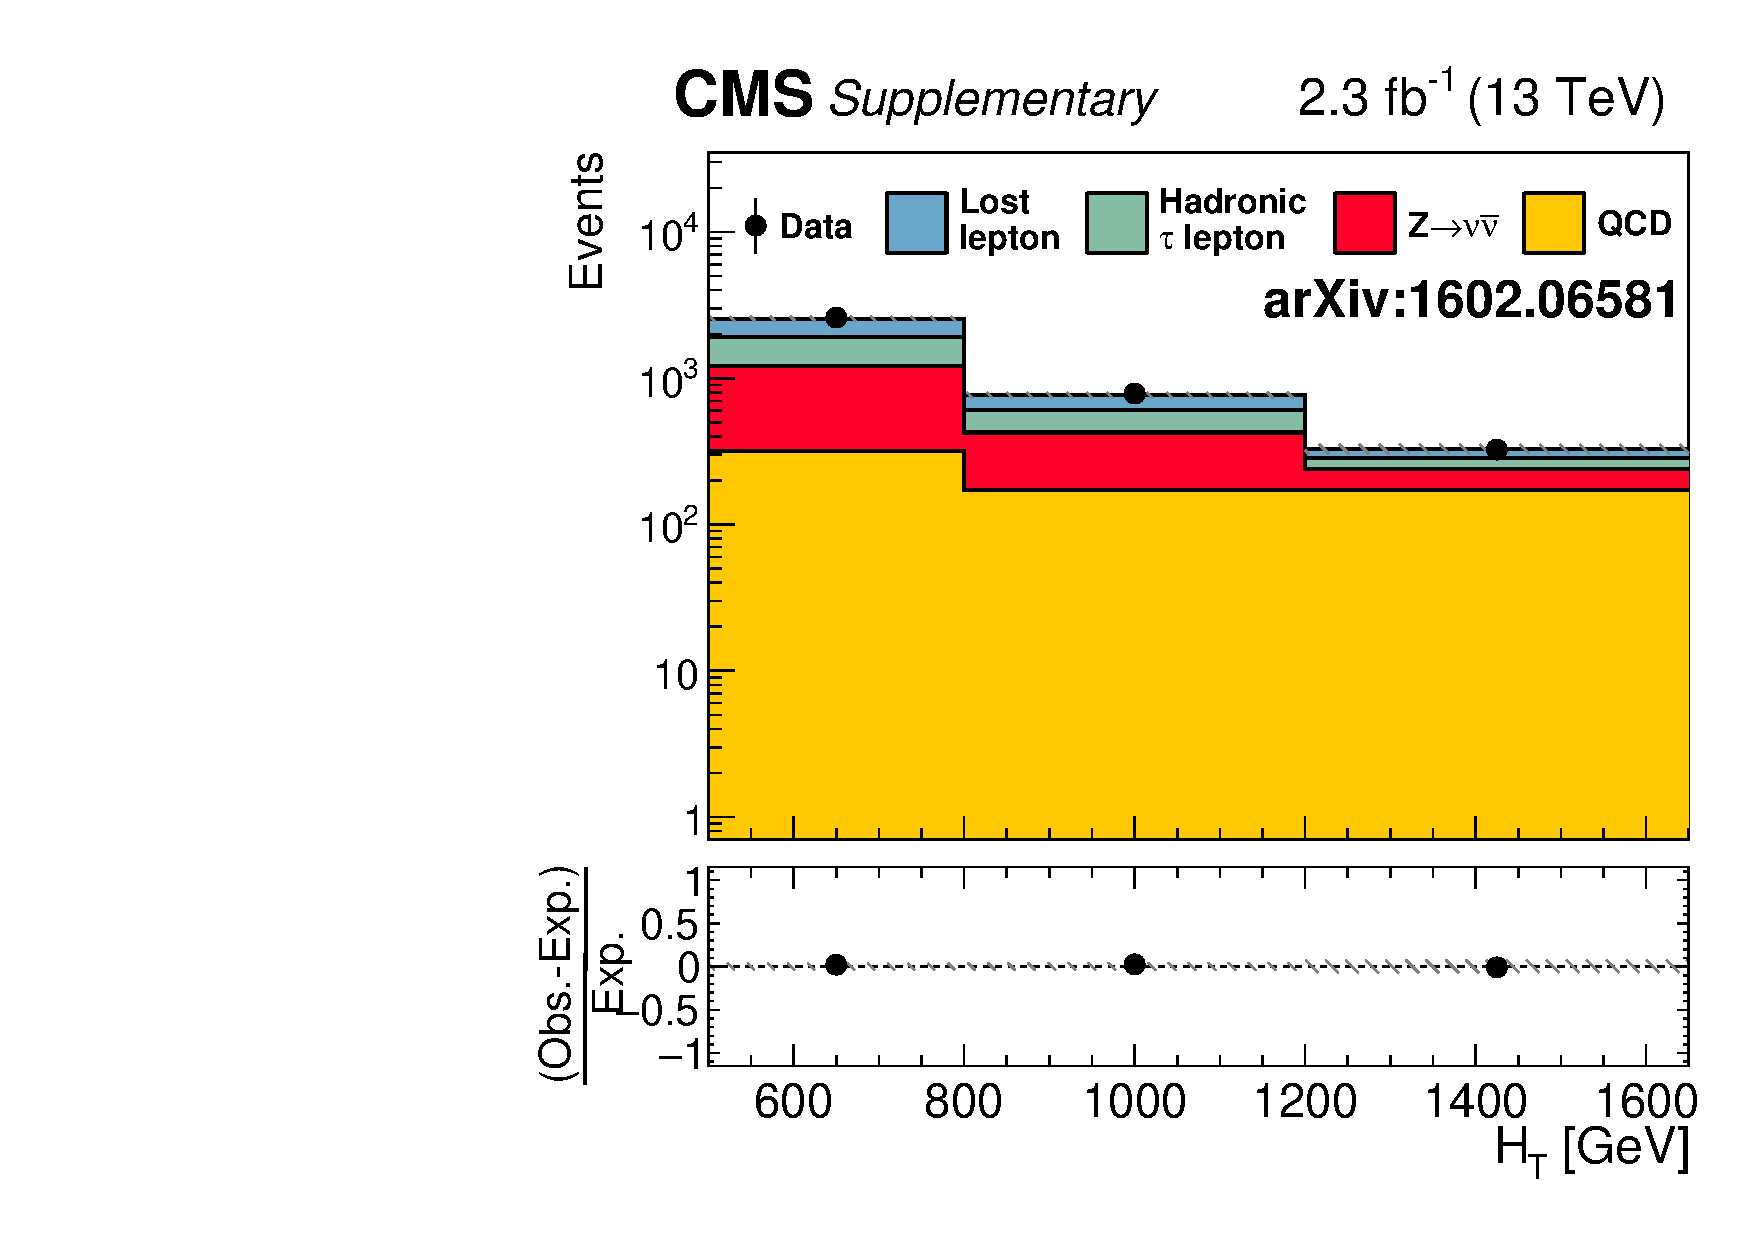
\includegraphics[width=0.48\textwidth]{1D-projection-allHT-log.pdf}
  \caption{
    The distributions of observed number of events and predicted background as a function of $H_{\rm T}$, plotted on linear (left) and log (right) scales. Distributions are integrated over other binned observables in the analysis, number of b-tagged jets, number of jets, and $H_{\rm T}^{\rm miss}$. 
  }
\end{figure}

\begin{figure}[htb]
  \centering
  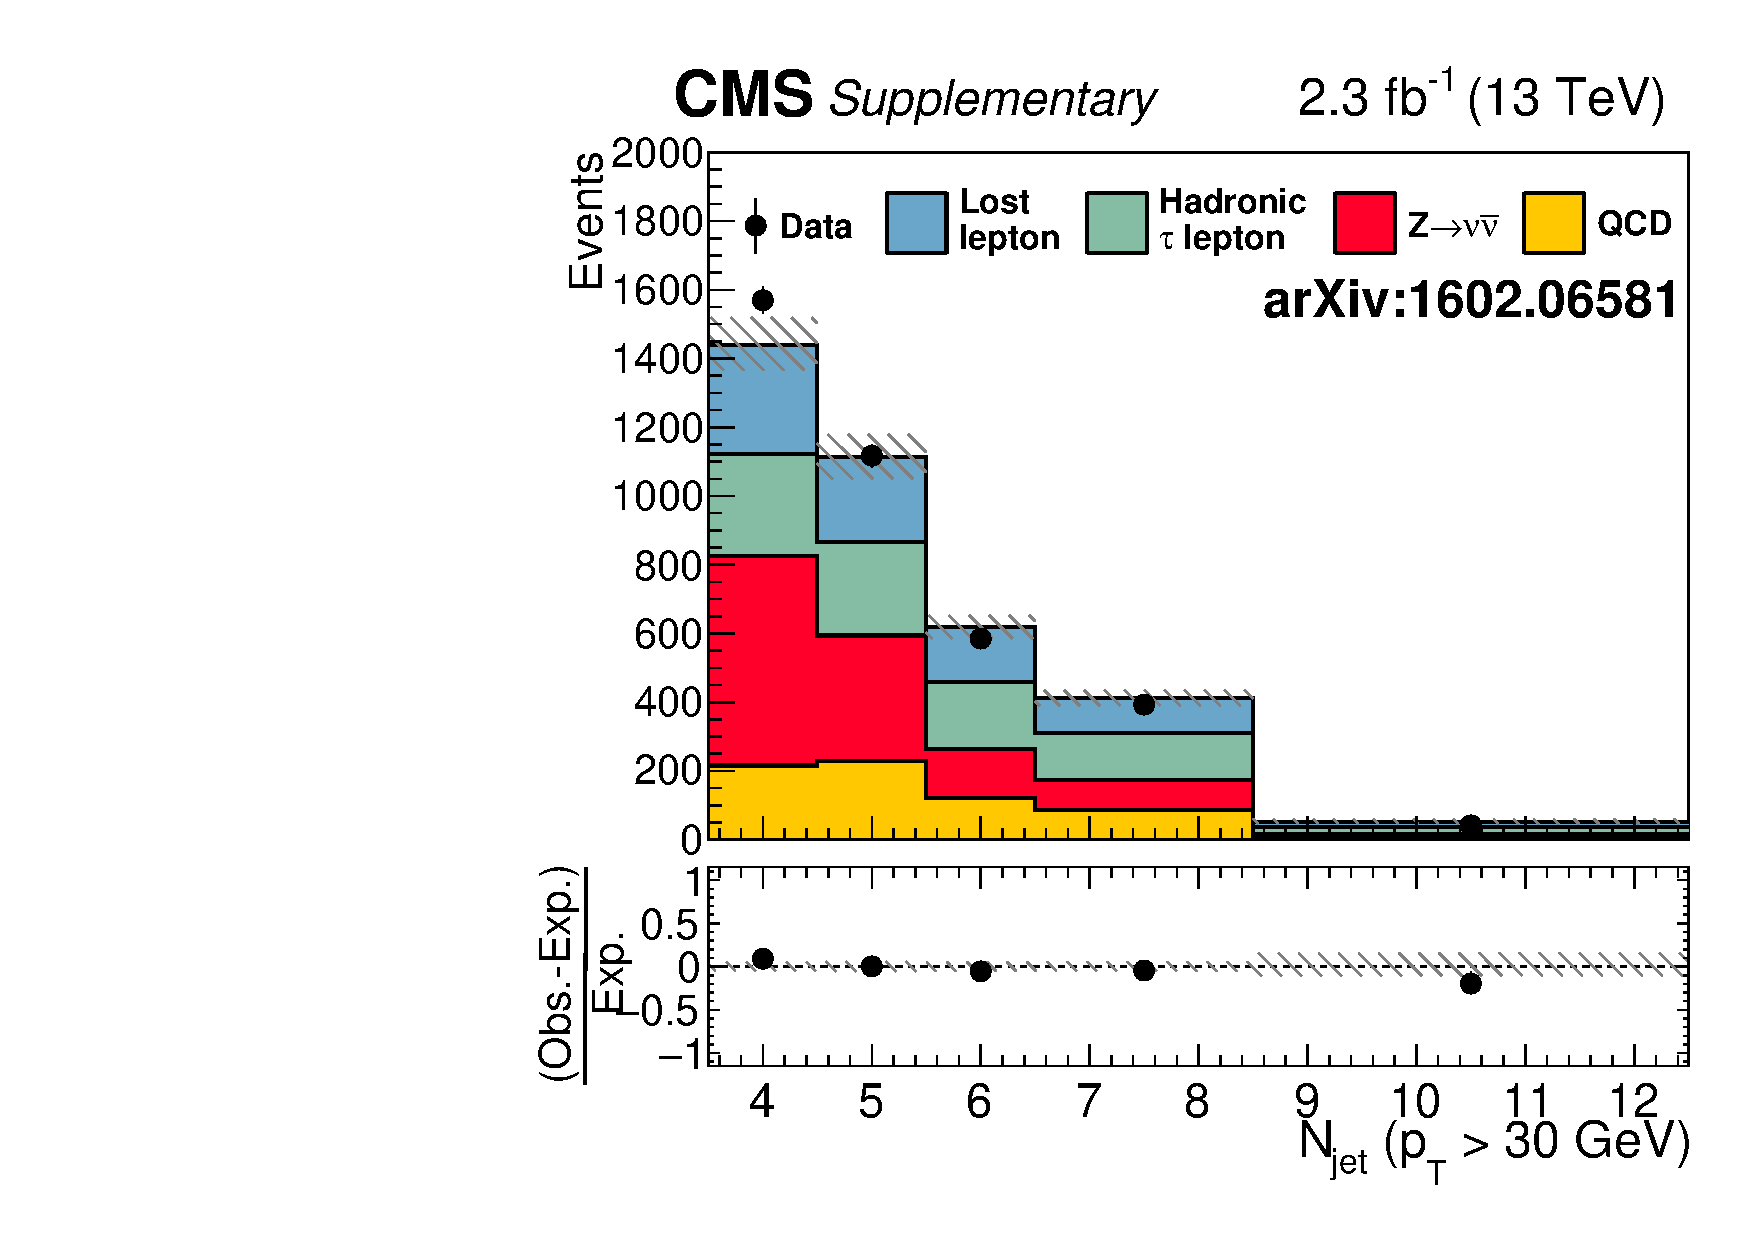
\includegraphics[width=0.48\textwidth]{1D-projection-allNJets.pdf}
  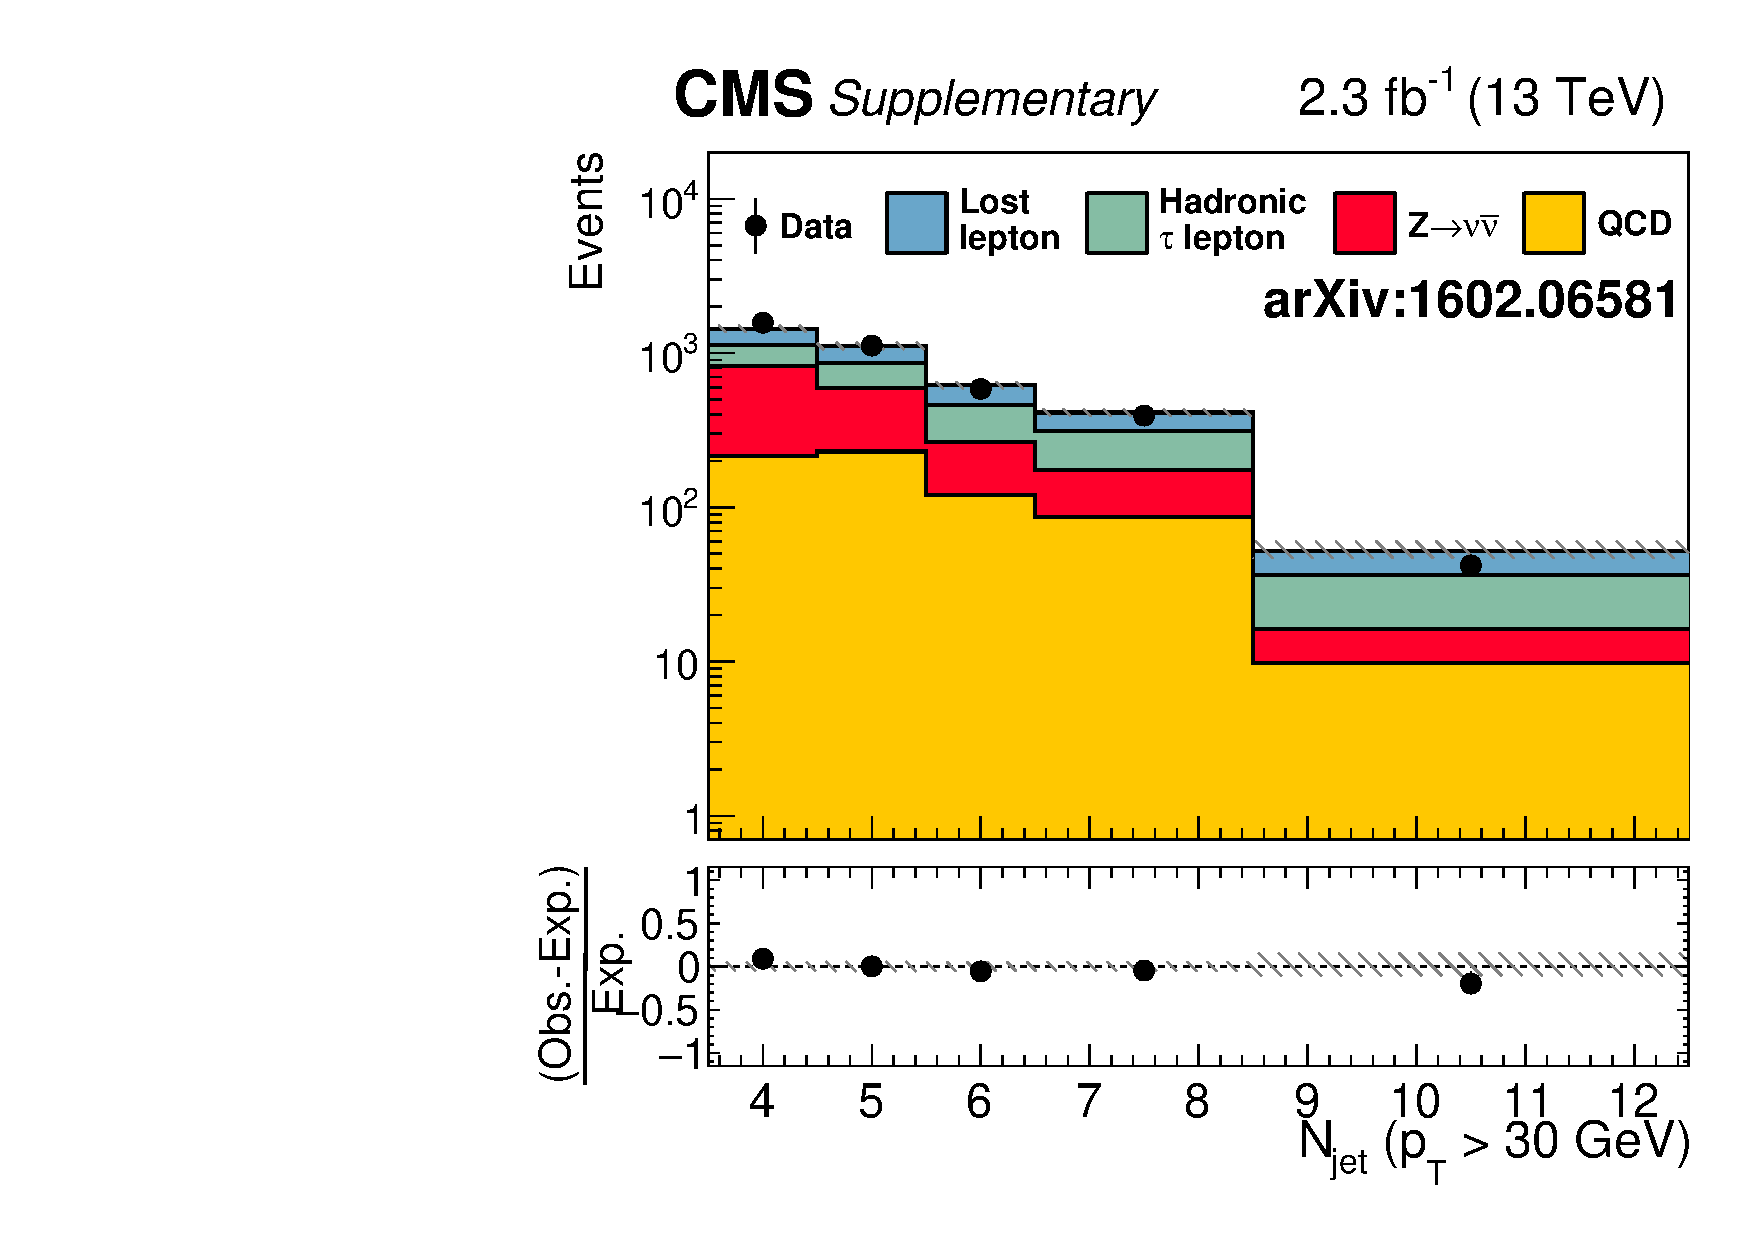
\includegraphics[width=0.48\textwidth]{1D-projection-allNJets-log.pdf}
  \caption{
    The distributions of observed number of events and predicted background as a function of the number of jets, plotted on linear (left) and log (right) scales. Distributions are integrated over other binned observables in the analysis, number of b-tagged jets, $H_{\rm T}^{\rm miss}$, and $H_{\rm T}$. 
  }
\end{figure}

\begin{figure}[htb]
  \centering
  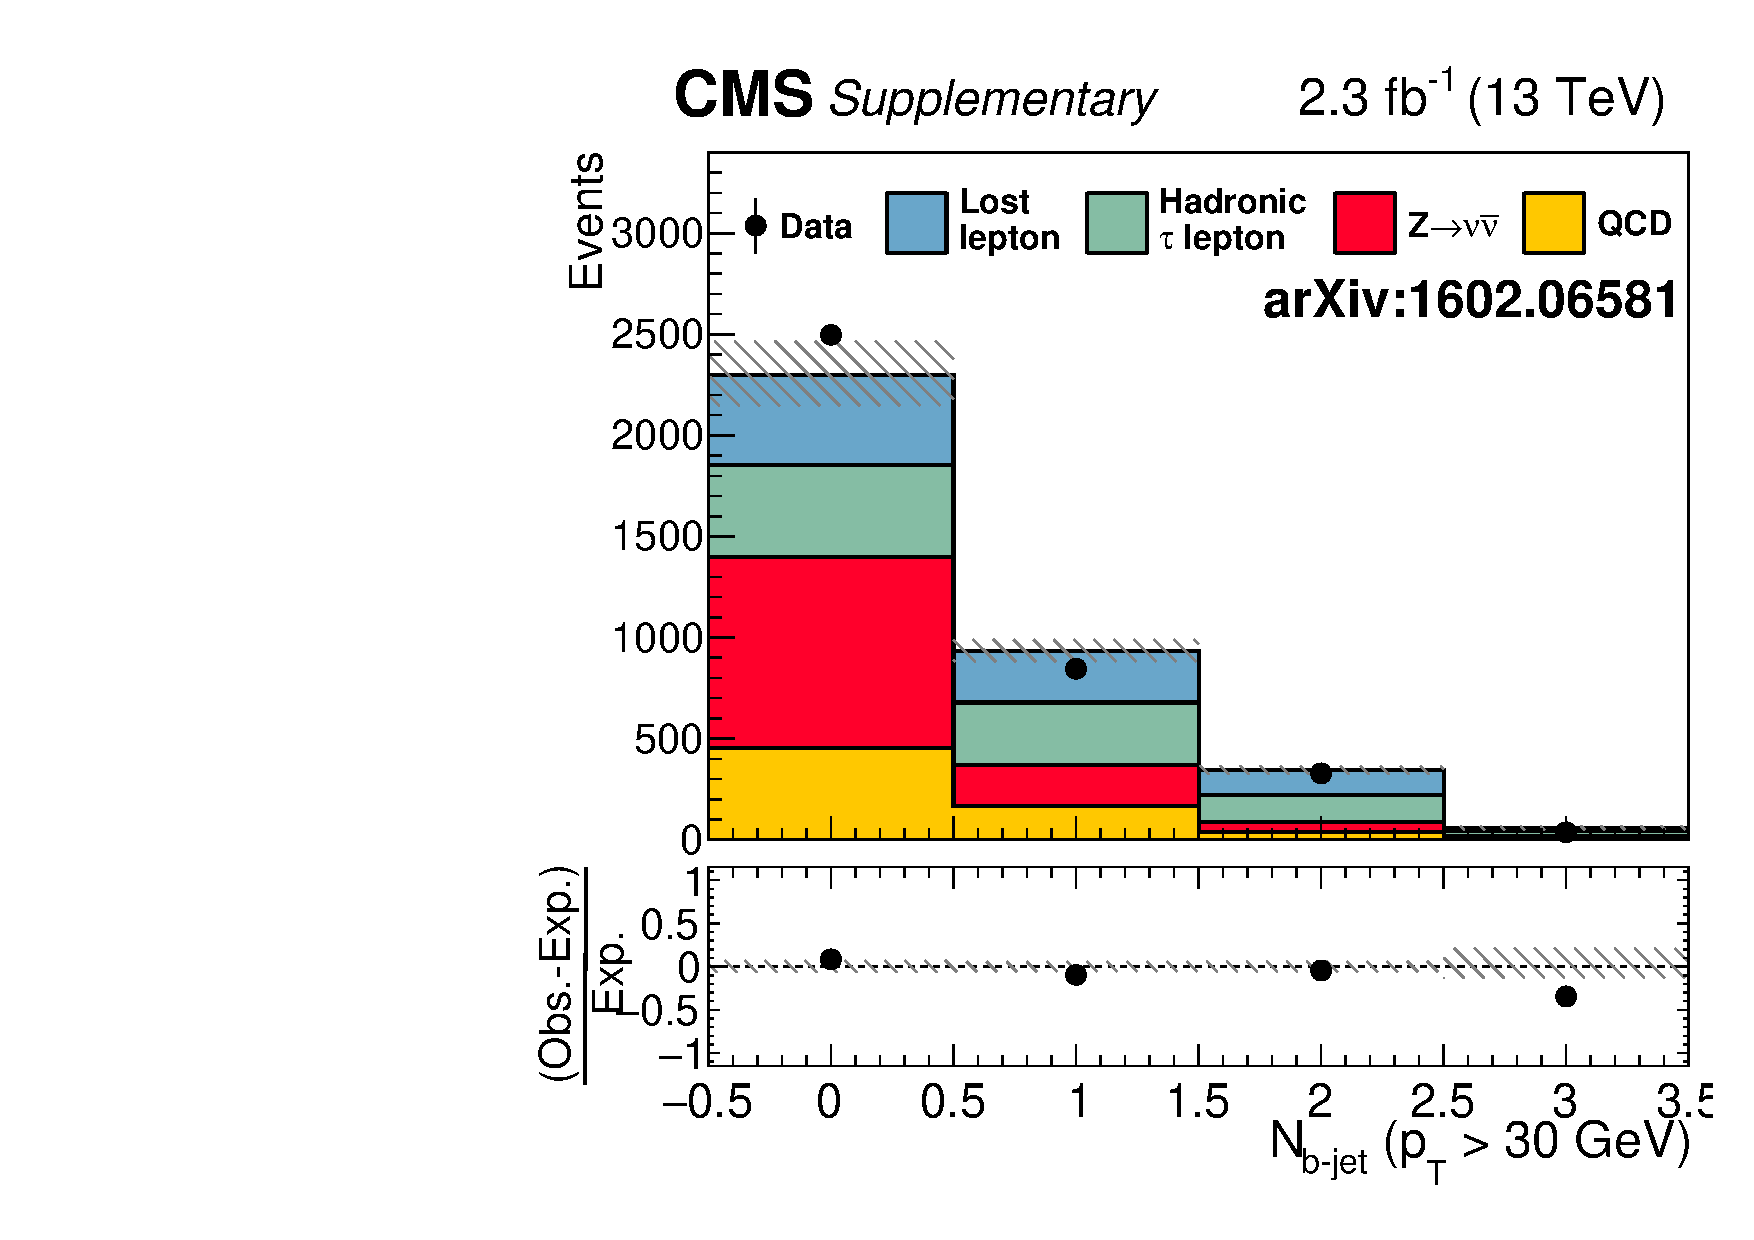
\includegraphics[width=0.48\textwidth]{1D-projection-allNBJets.pdf}
  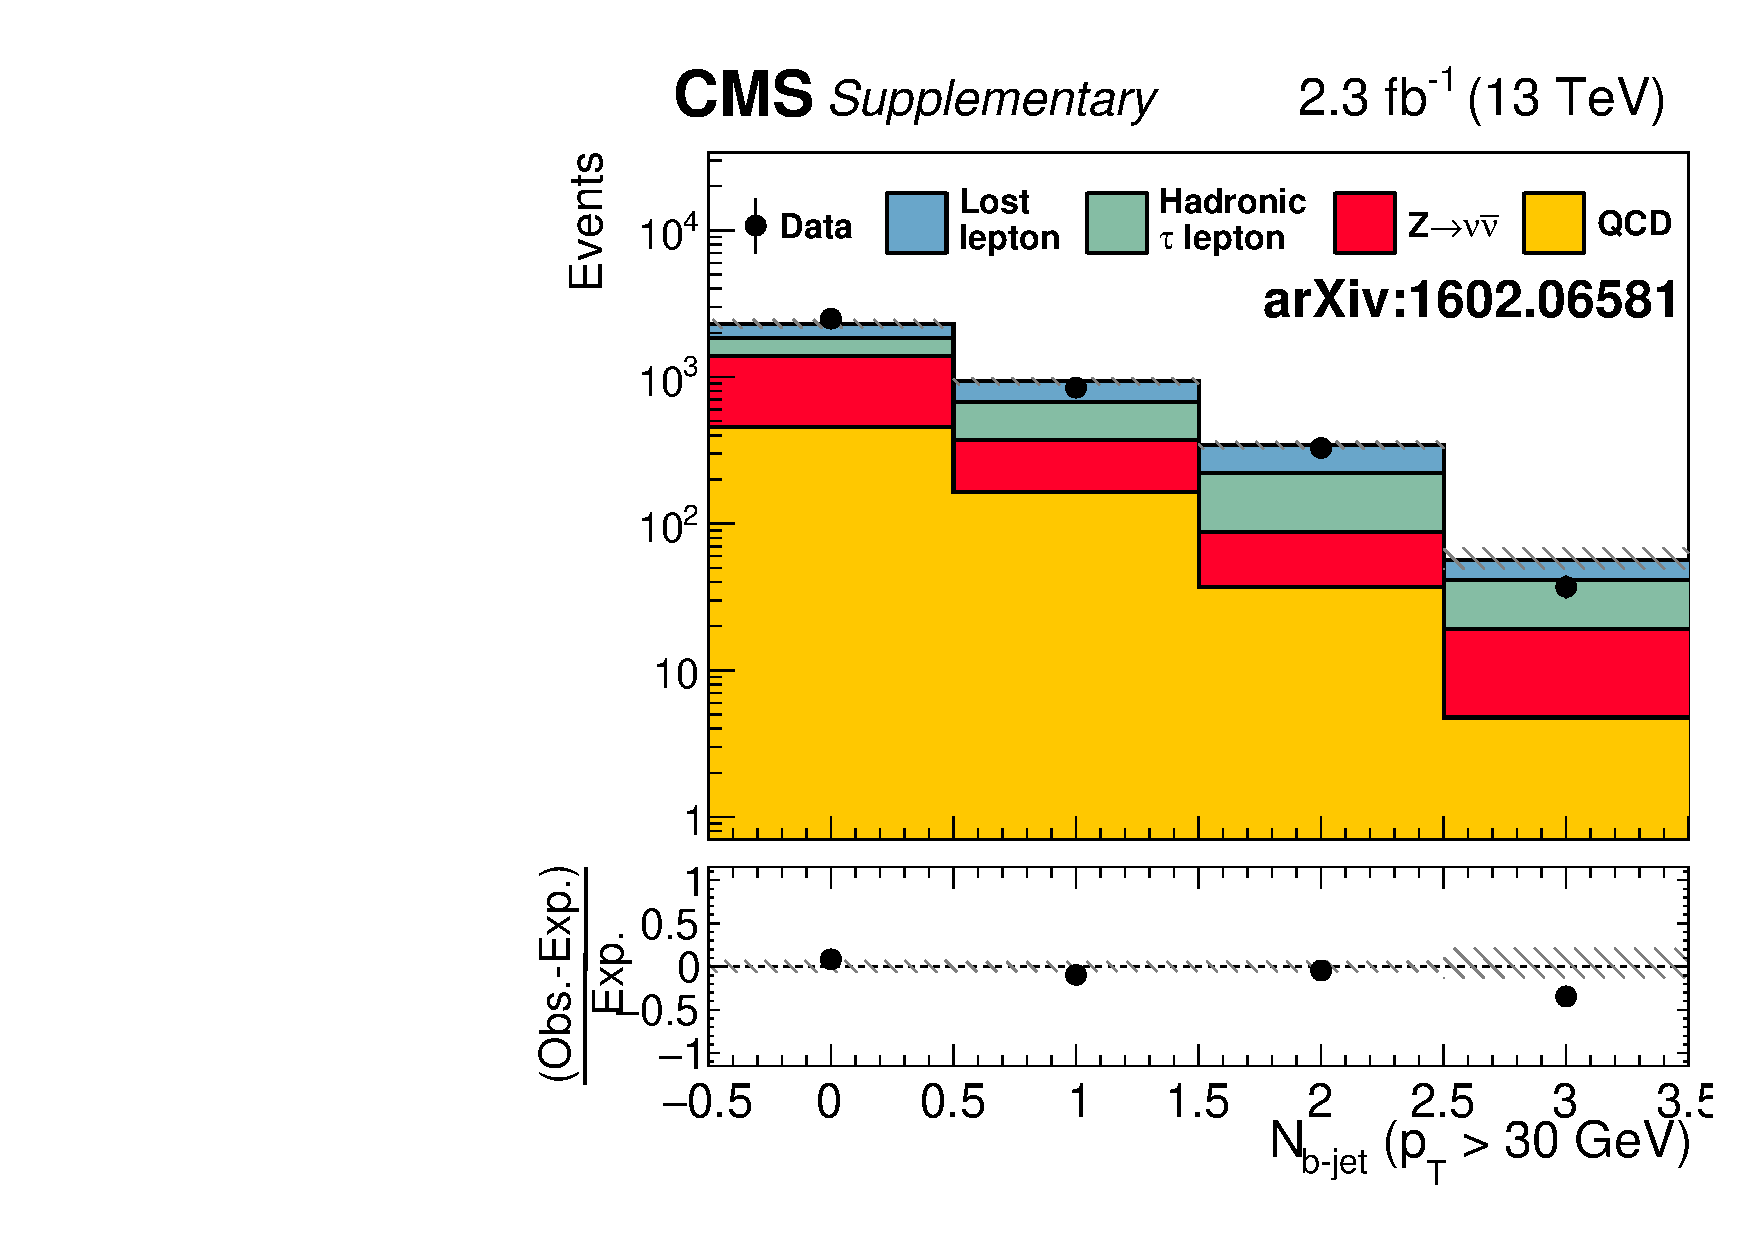
\includegraphics[width=0.48\textwidth]{1D-projection-allNBJets-log.pdf}
  \caption{
    The distributions of observed number of events and predicted background as a function of the number of b-tagged jets, plotted on linear (left) and log (right) scales. Distributions are integrated over other binned observables in the analysis, number of jets, $H_{\rm T}^{\rm miss}$, and $H_{\rm T}$. 
  }
\end{figure}

\begin{figure}[htb]
  \centering
  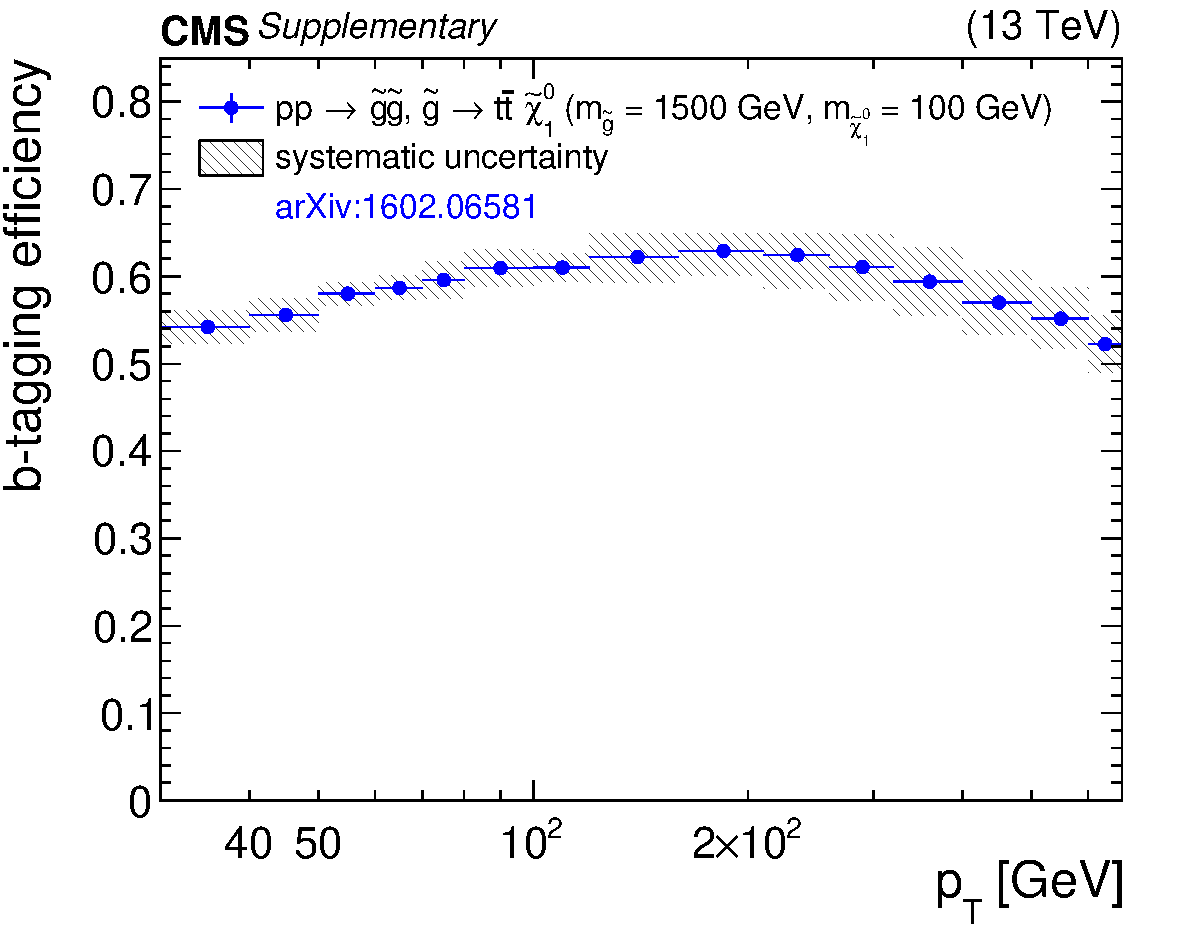
\includegraphics[width=0.9\textwidth]{effb_T1tttt_1500_100.pdf}
  \caption{
    The b-tagging efficiency, with data/MC scale factors applied, for a representative signal model. Statistical and systematic uncertainties are shown separately. 
  }
\end{figure}

\begin{figure}[htb]
  \centering
  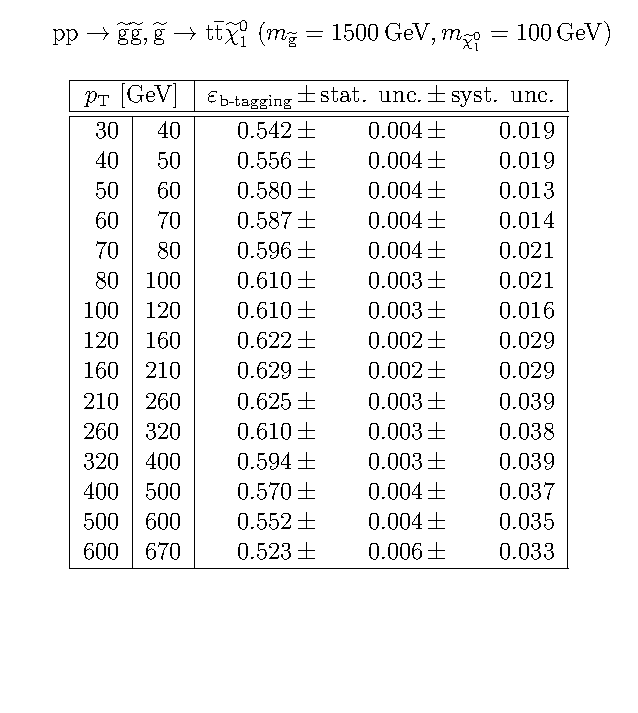
\includegraphics[width=0.9\textwidth]{effb.pdf}
  \caption{
    The b-tagging efficiency in table form, with data/MC scale factors applied, for a representative signal model. Statistical and systematic uncertainties are shown separately. 
  }
\end{figure}

\begin{figure}[htb]
  \centering
  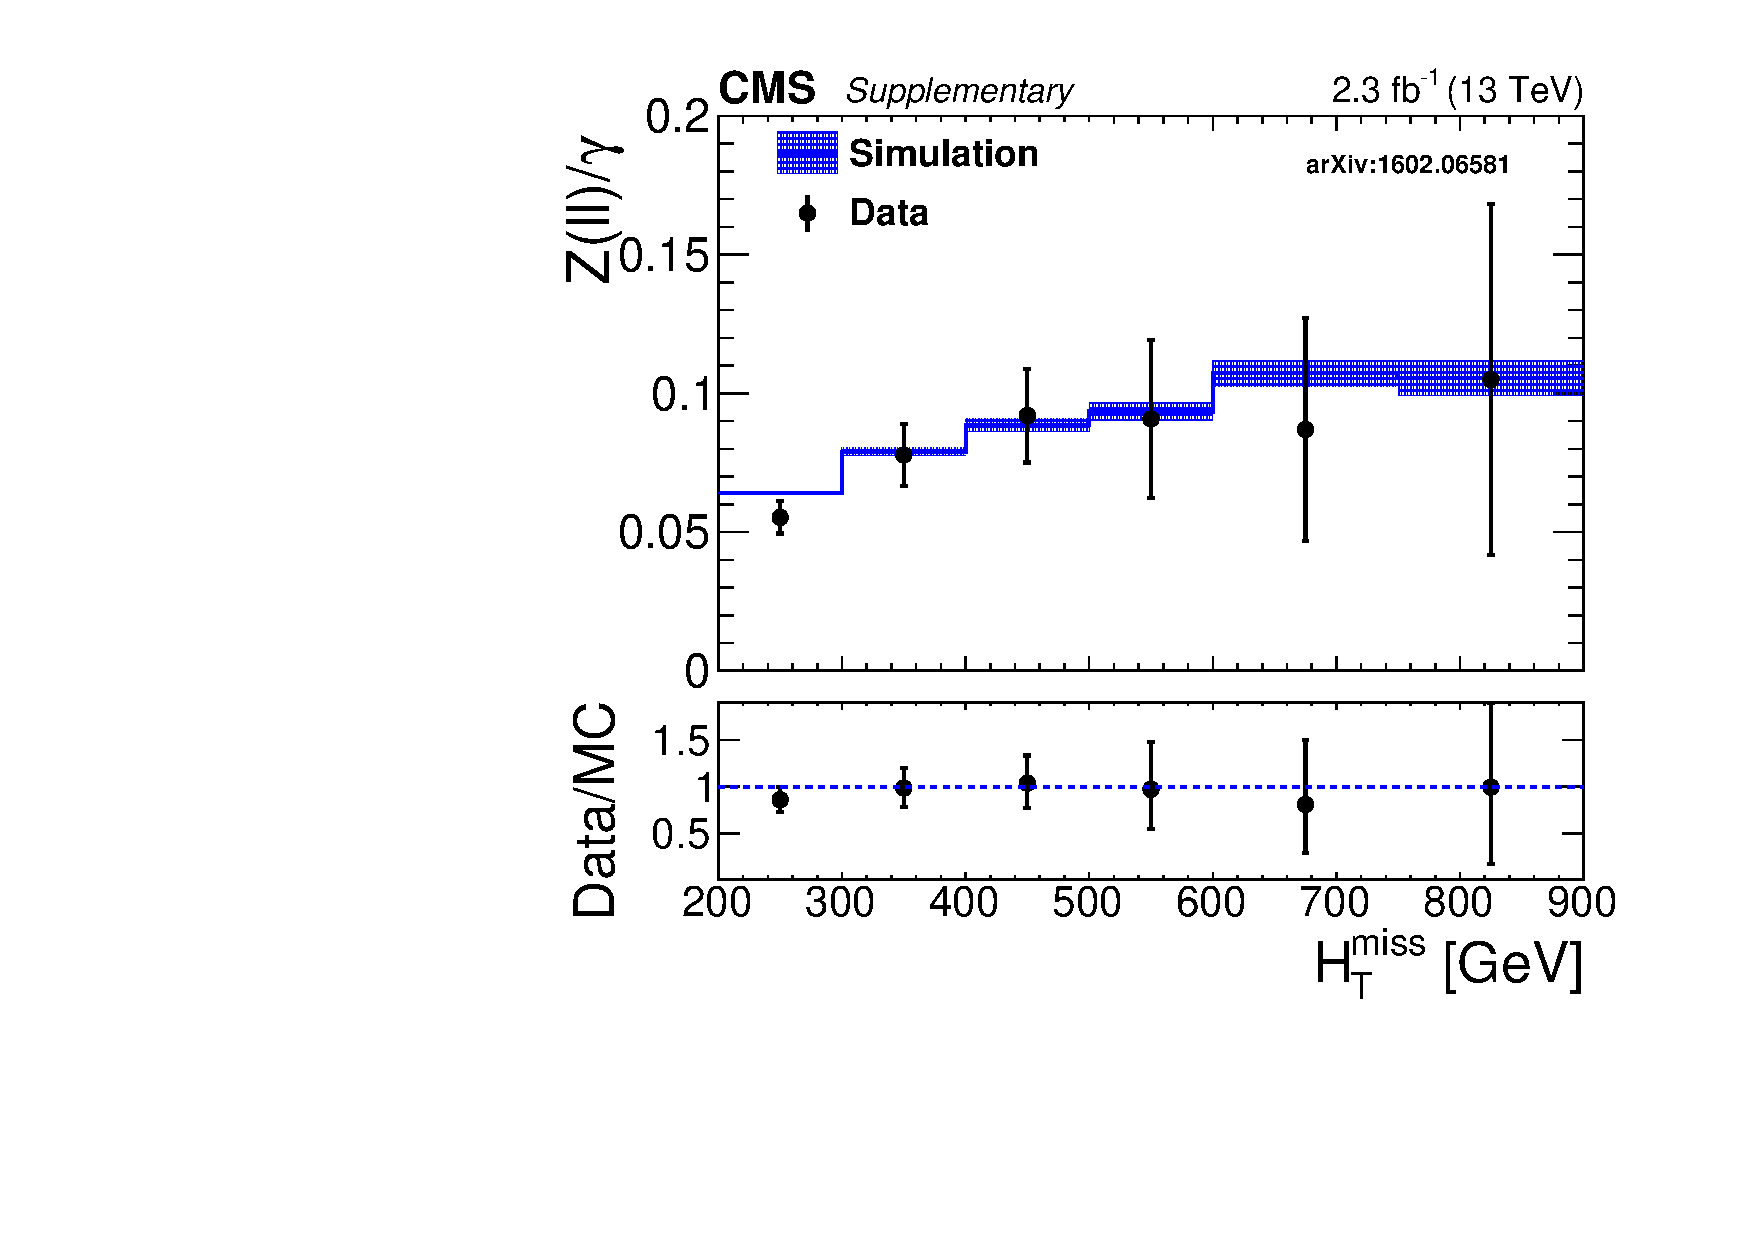
\includegraphics[width=0.3\textwidth]{dr_mht_talk_sup.pdf}
  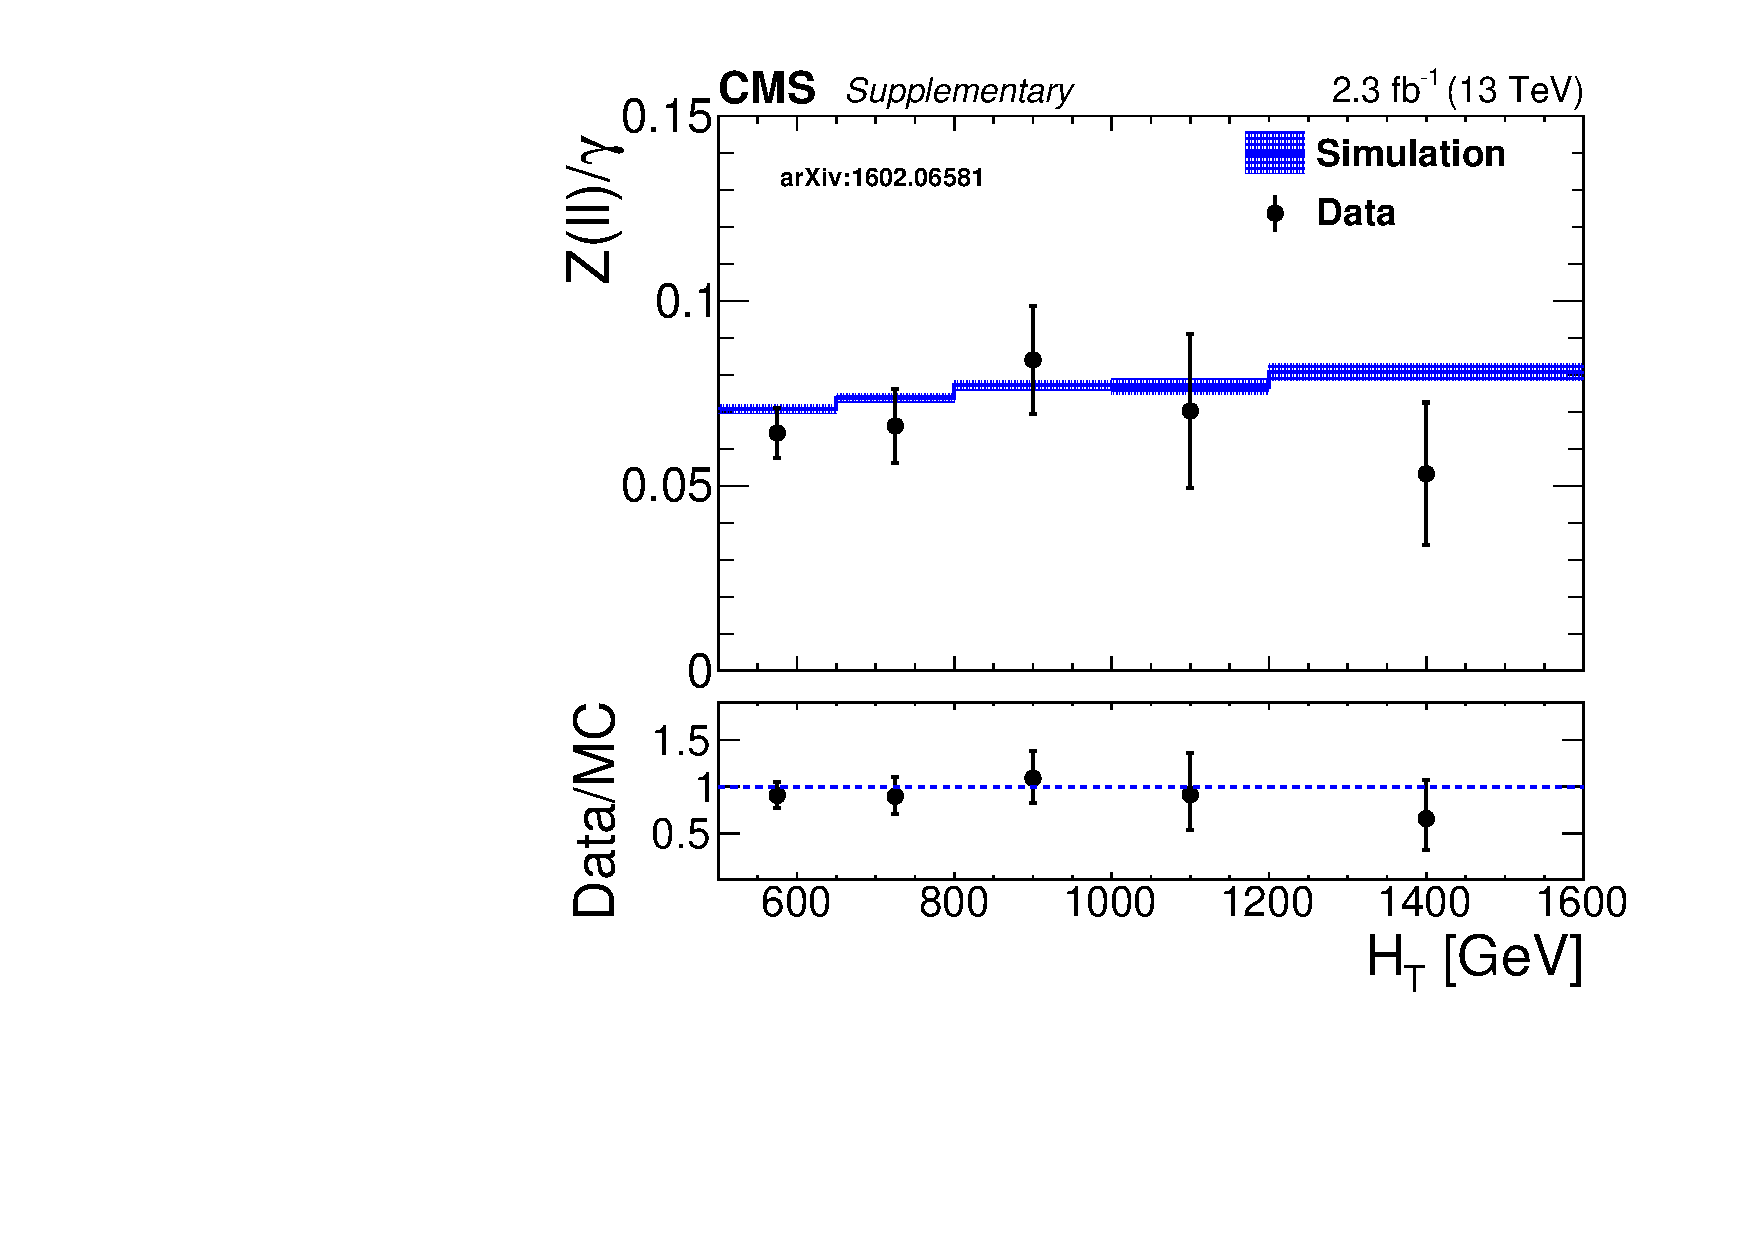
\includegraphics[width=0.3\textwidth]{dr_ht_talk_sup.pdf}
  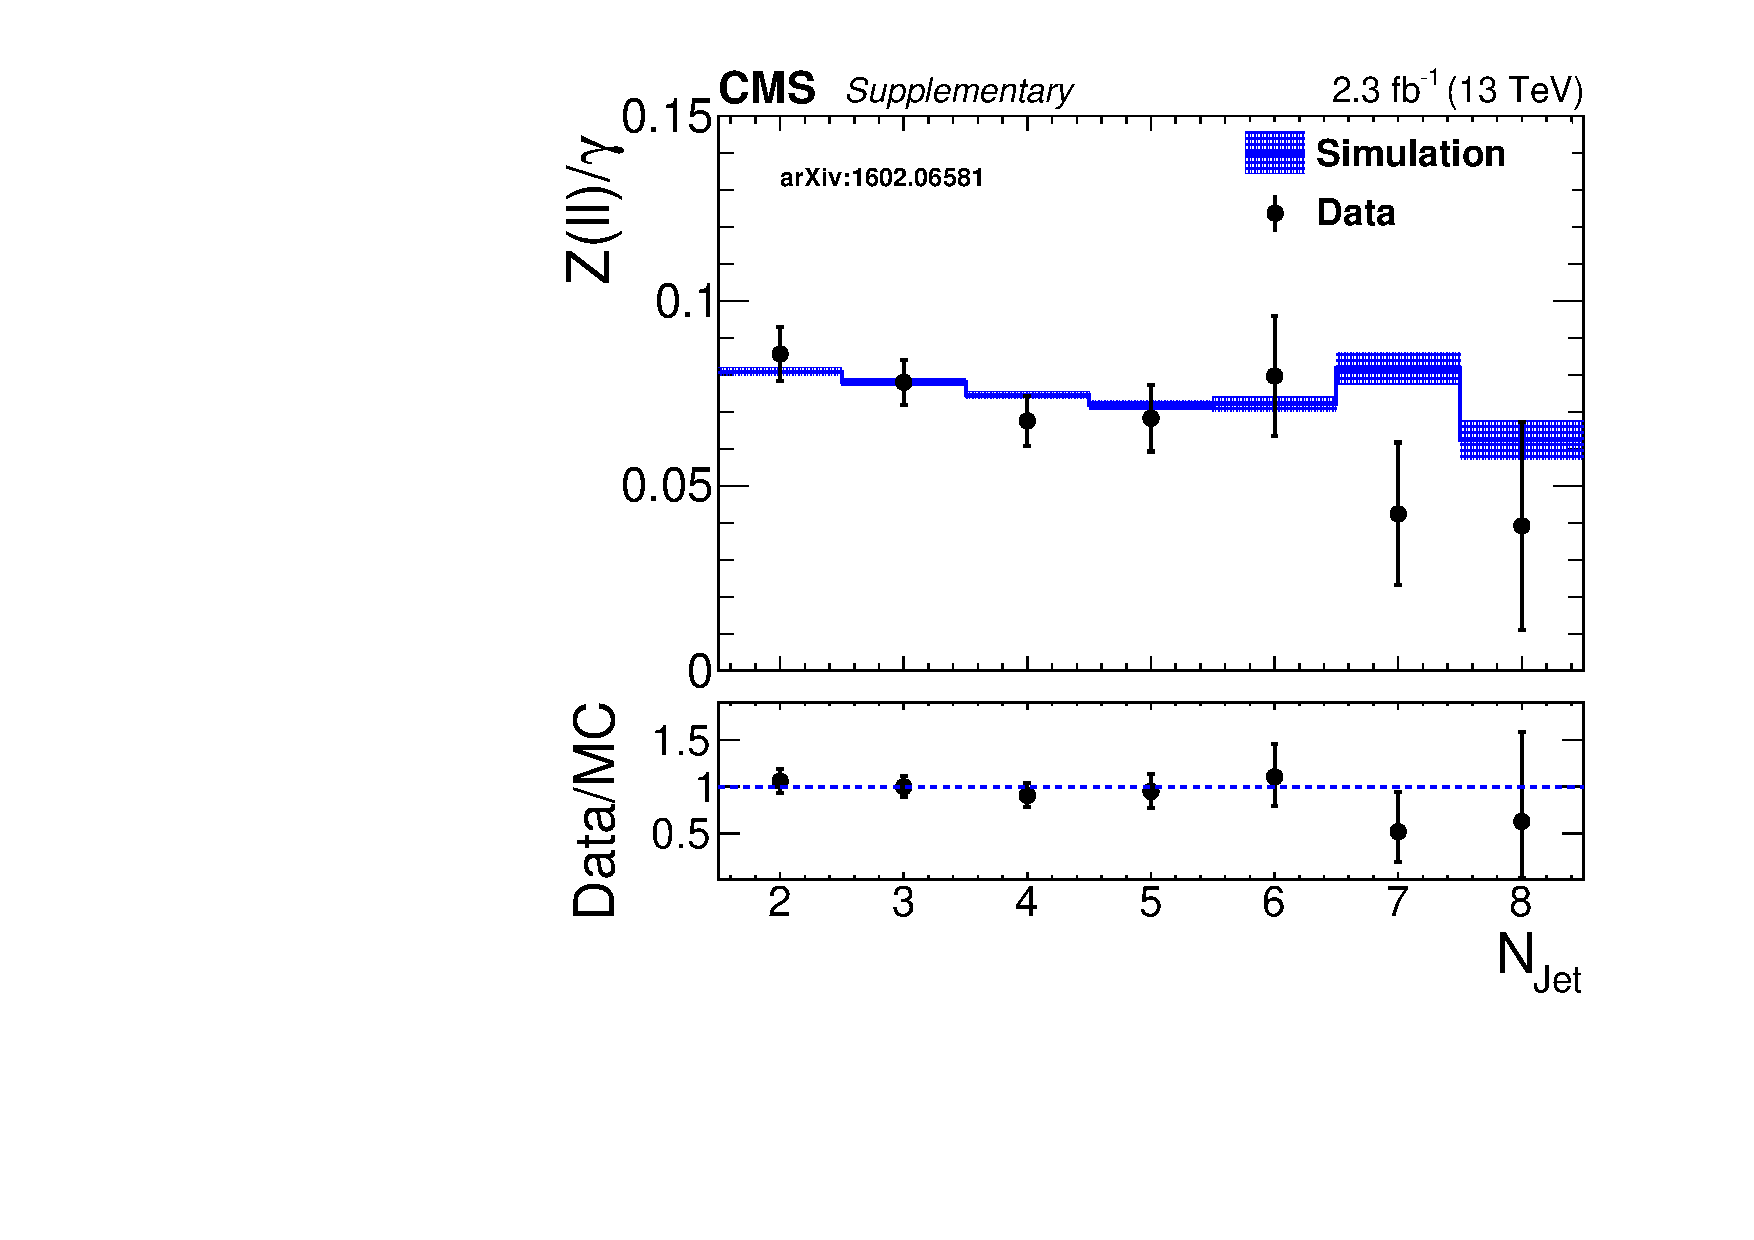
\includegraphics[width=0.3\textwidth]{dr_nj_talk_sup.pdf}
  \caption{
The $Z\rightarrow\ell^+\ell^-/\gamma$ ratio as a function of $H_{\rm T}^{\rm miss}$ (left), $H_{\rm T}$ (middle), and the number of jets (right) after baseline selection. The $Z\rightarrow\nu\bar{\nu}/\gamma$ transfer factor is computed using simulated events and we check in one dimensional projections that data agree with simulation. 
  }
\end{figure}


\begin{figure}[htb]
  \centering
  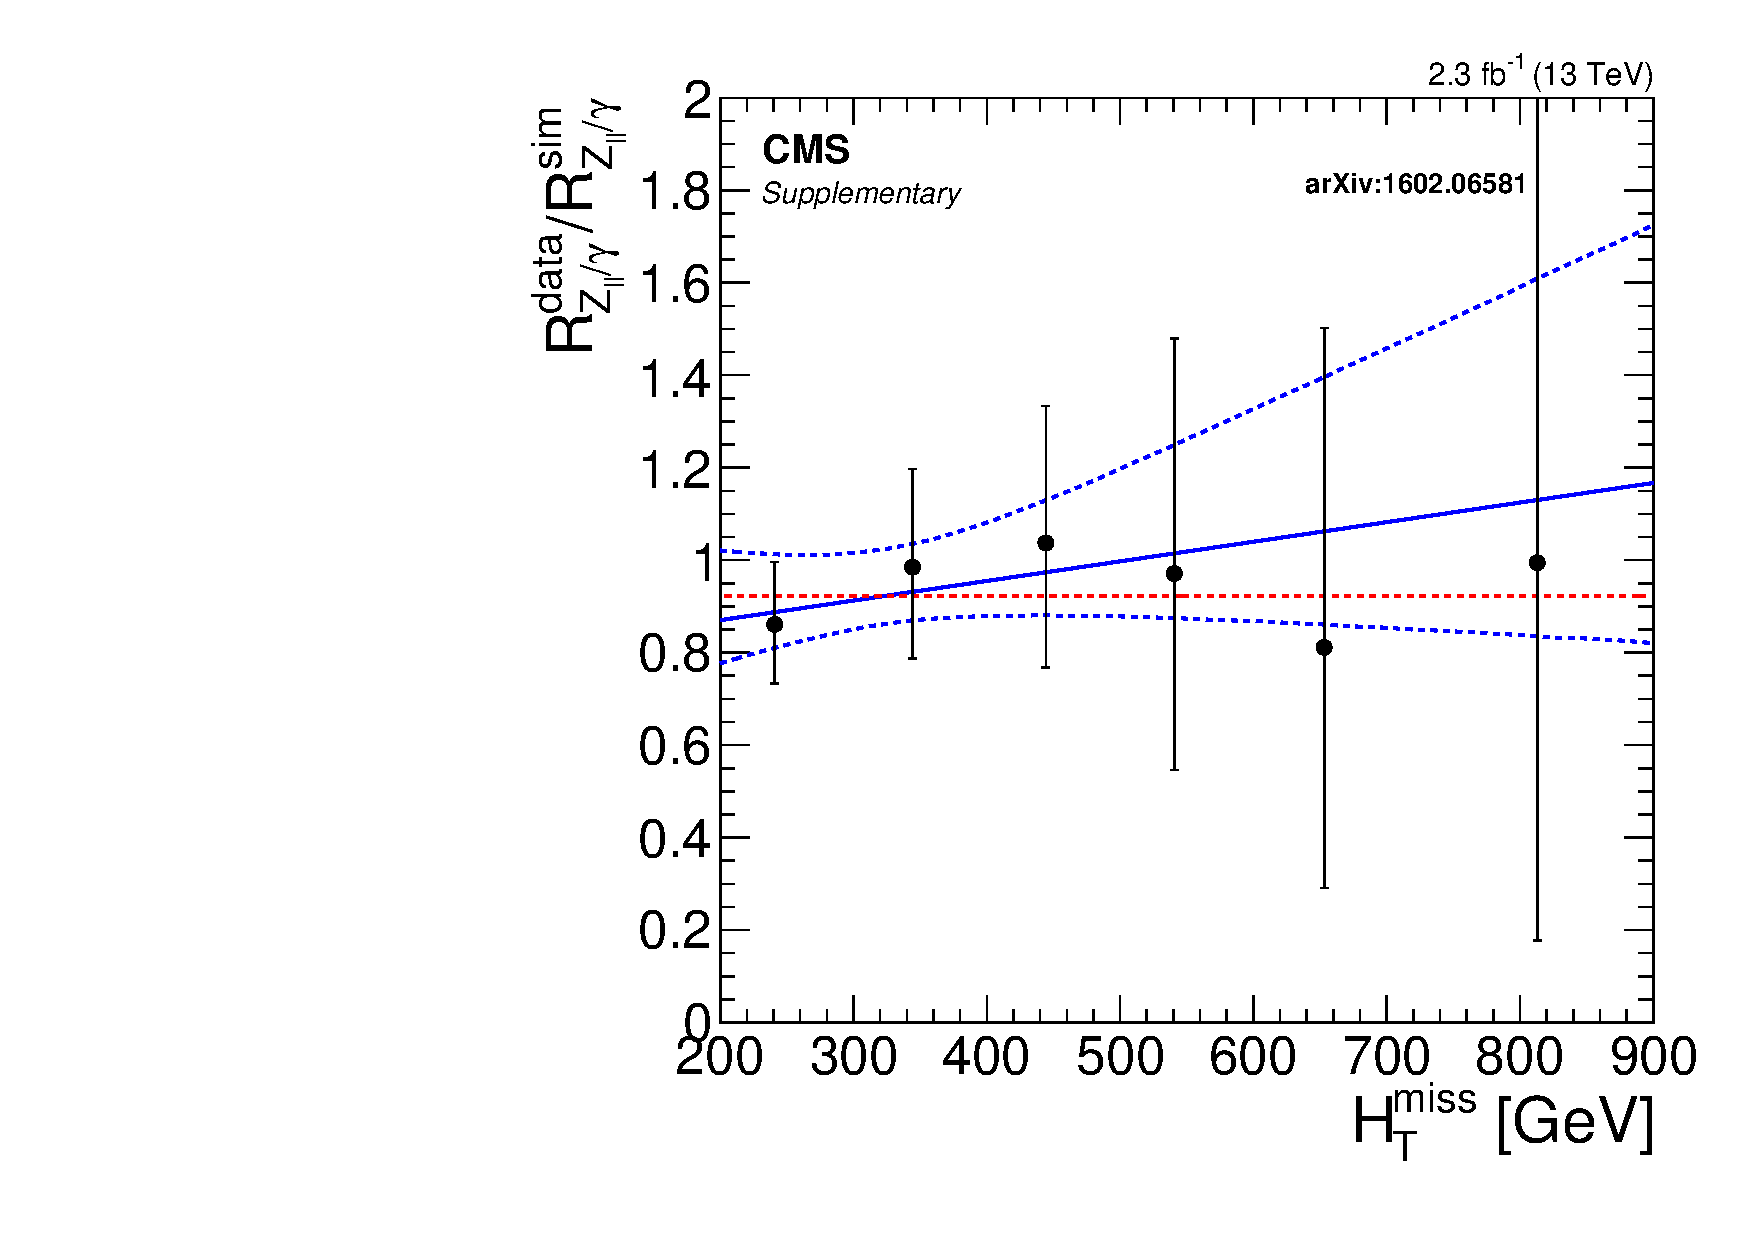
\includegraphics[width=0.3\textwidth]{dr_mht.pdf}
  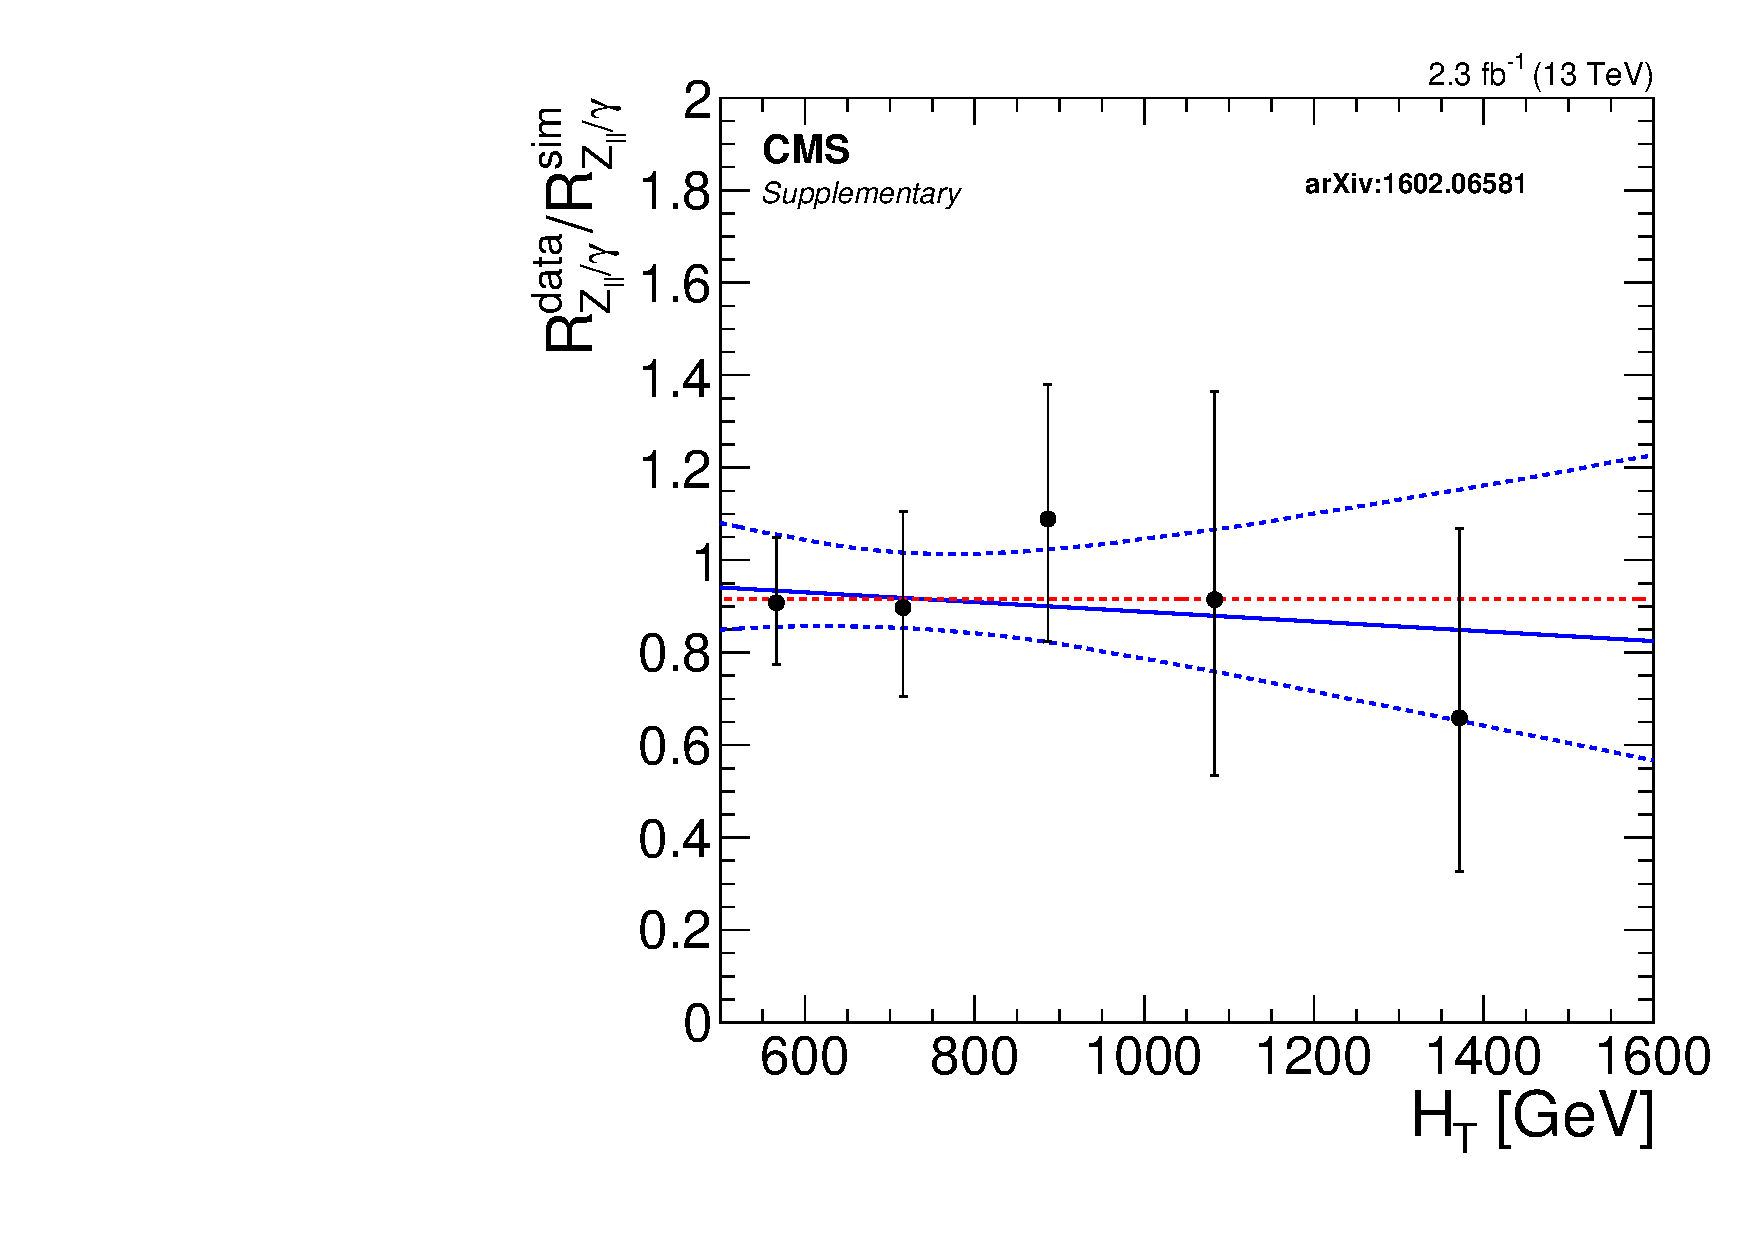
\includegraphics[width=0.3\textwidth]{dr_ht.pdf}
  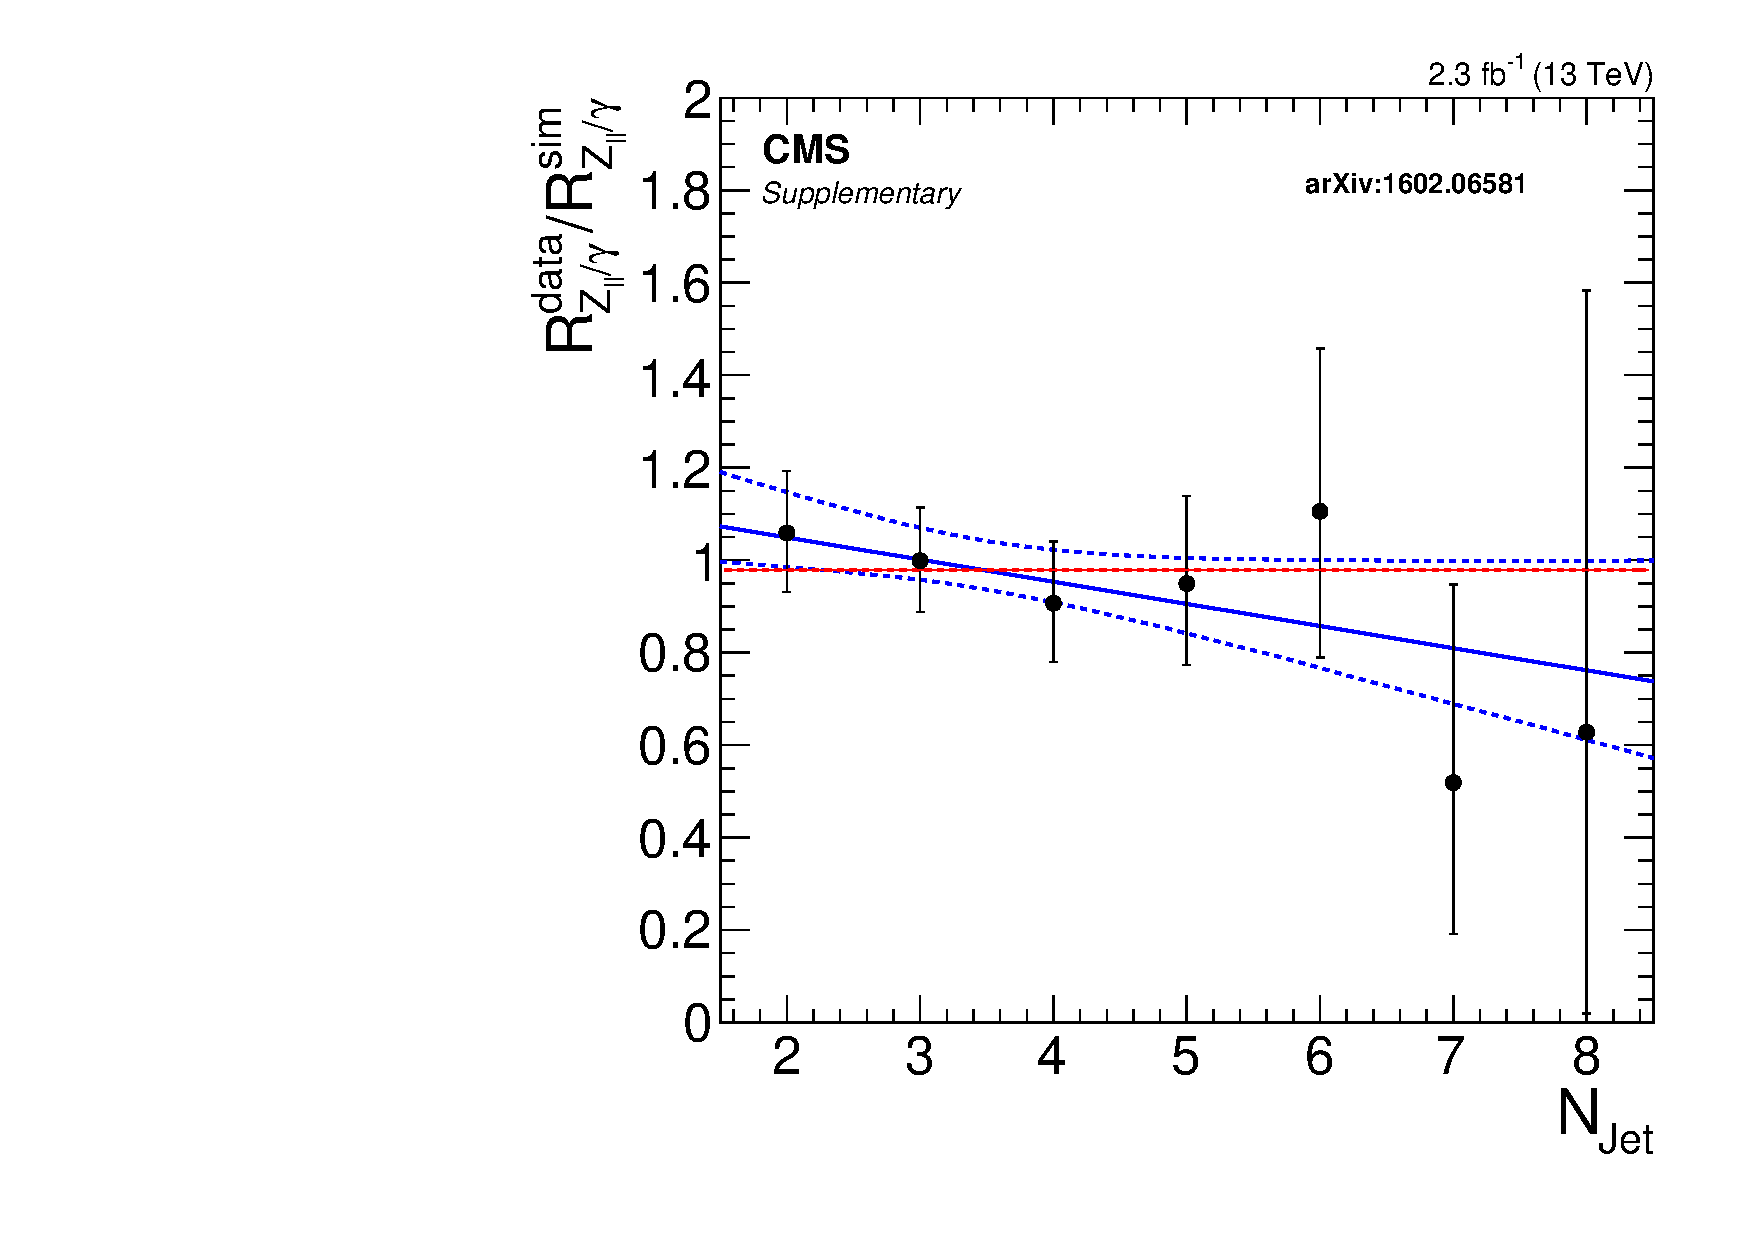
\includegraphics[width=0.3\textwidth]{dr_njet.pdf}
  \caption{
    The $Z\rightarrow\ell^+\ell^-/\gamma$ Double Ratio and linear fit as a function of $H_{\rm T}^{\rm miss}$ (left), $H_{\rm T}$ (middle), and the number of jets (right) after baseline selection. The average value of 0.924 is drawn as a red dashed line. 
  }
\end{figure}

\begin{figure}[htb]
  \centering
  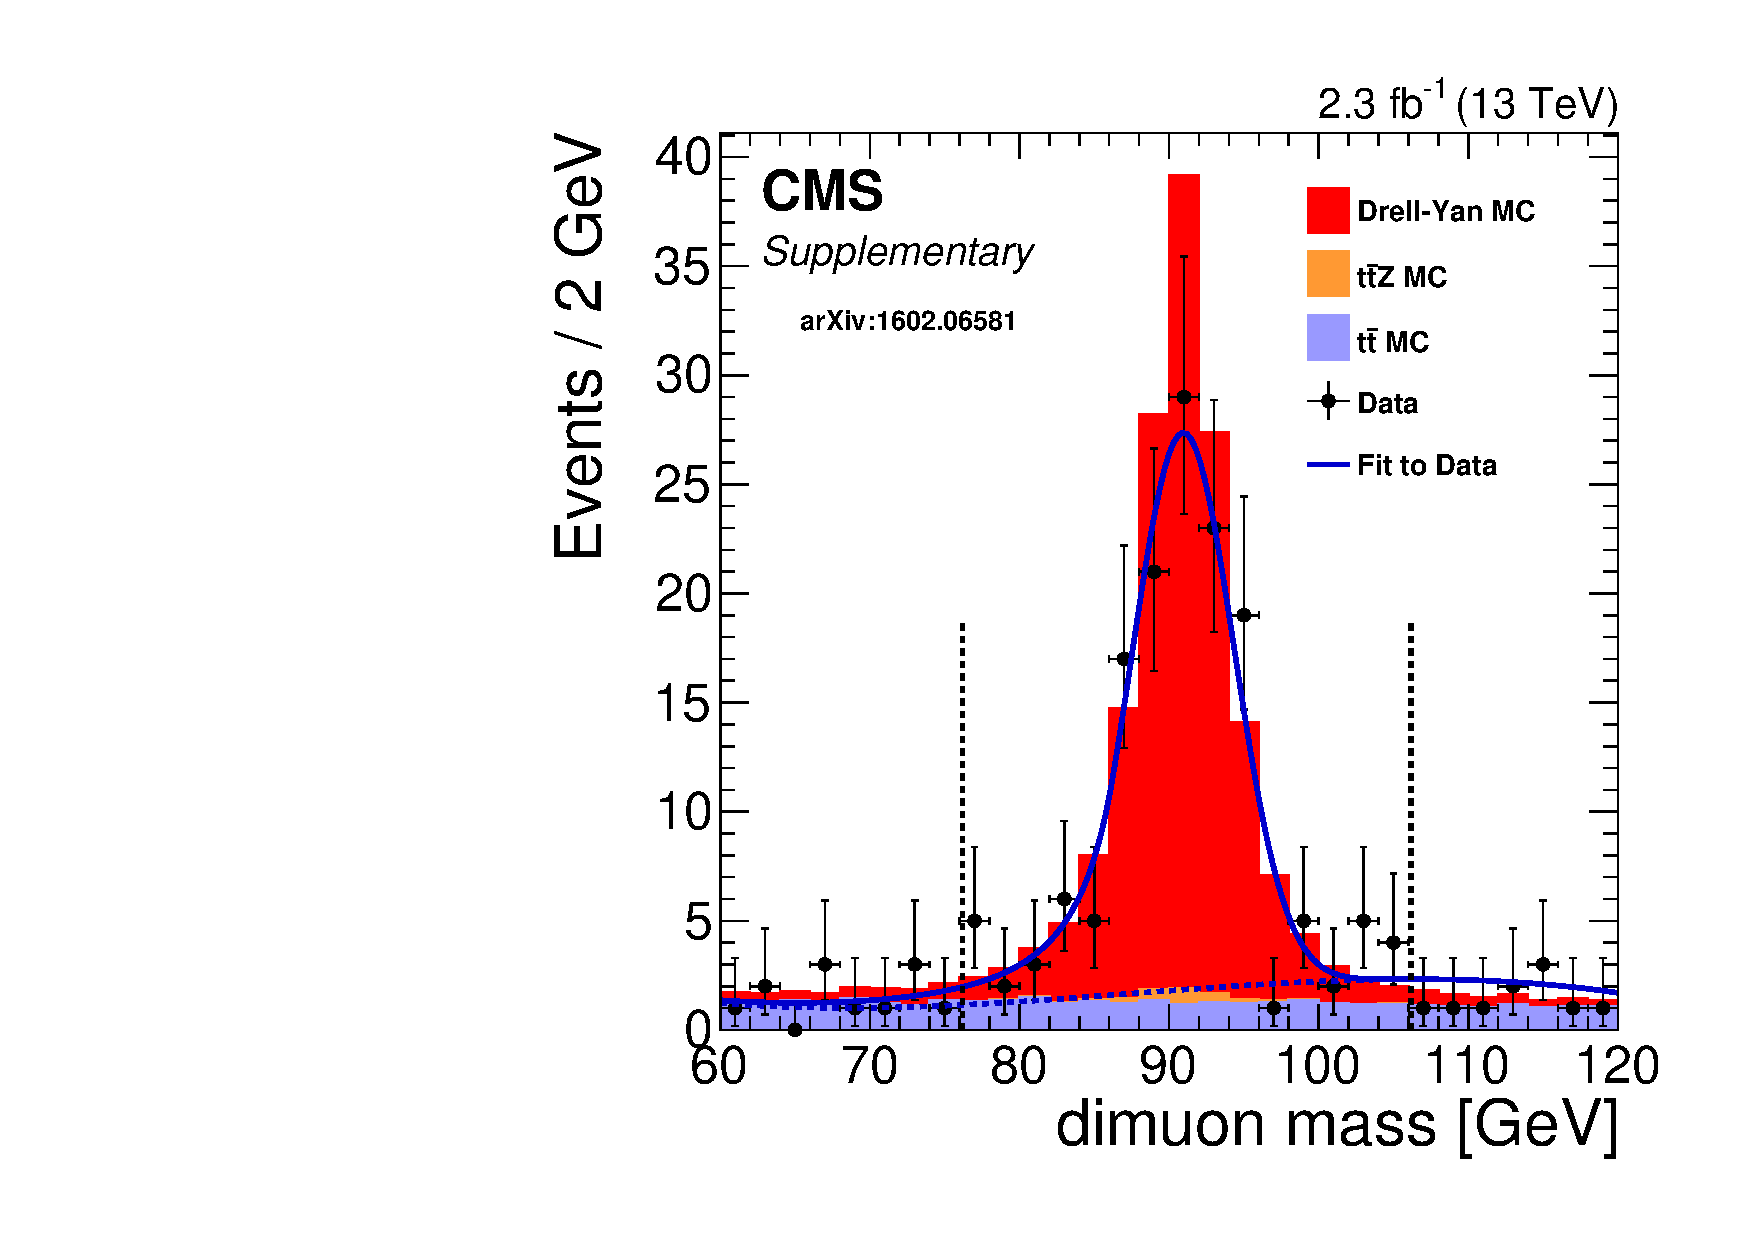
\includegraphics[width=0.48\textwidth]{mm_nJ-1_bJ-1_kin-1.pdf}
  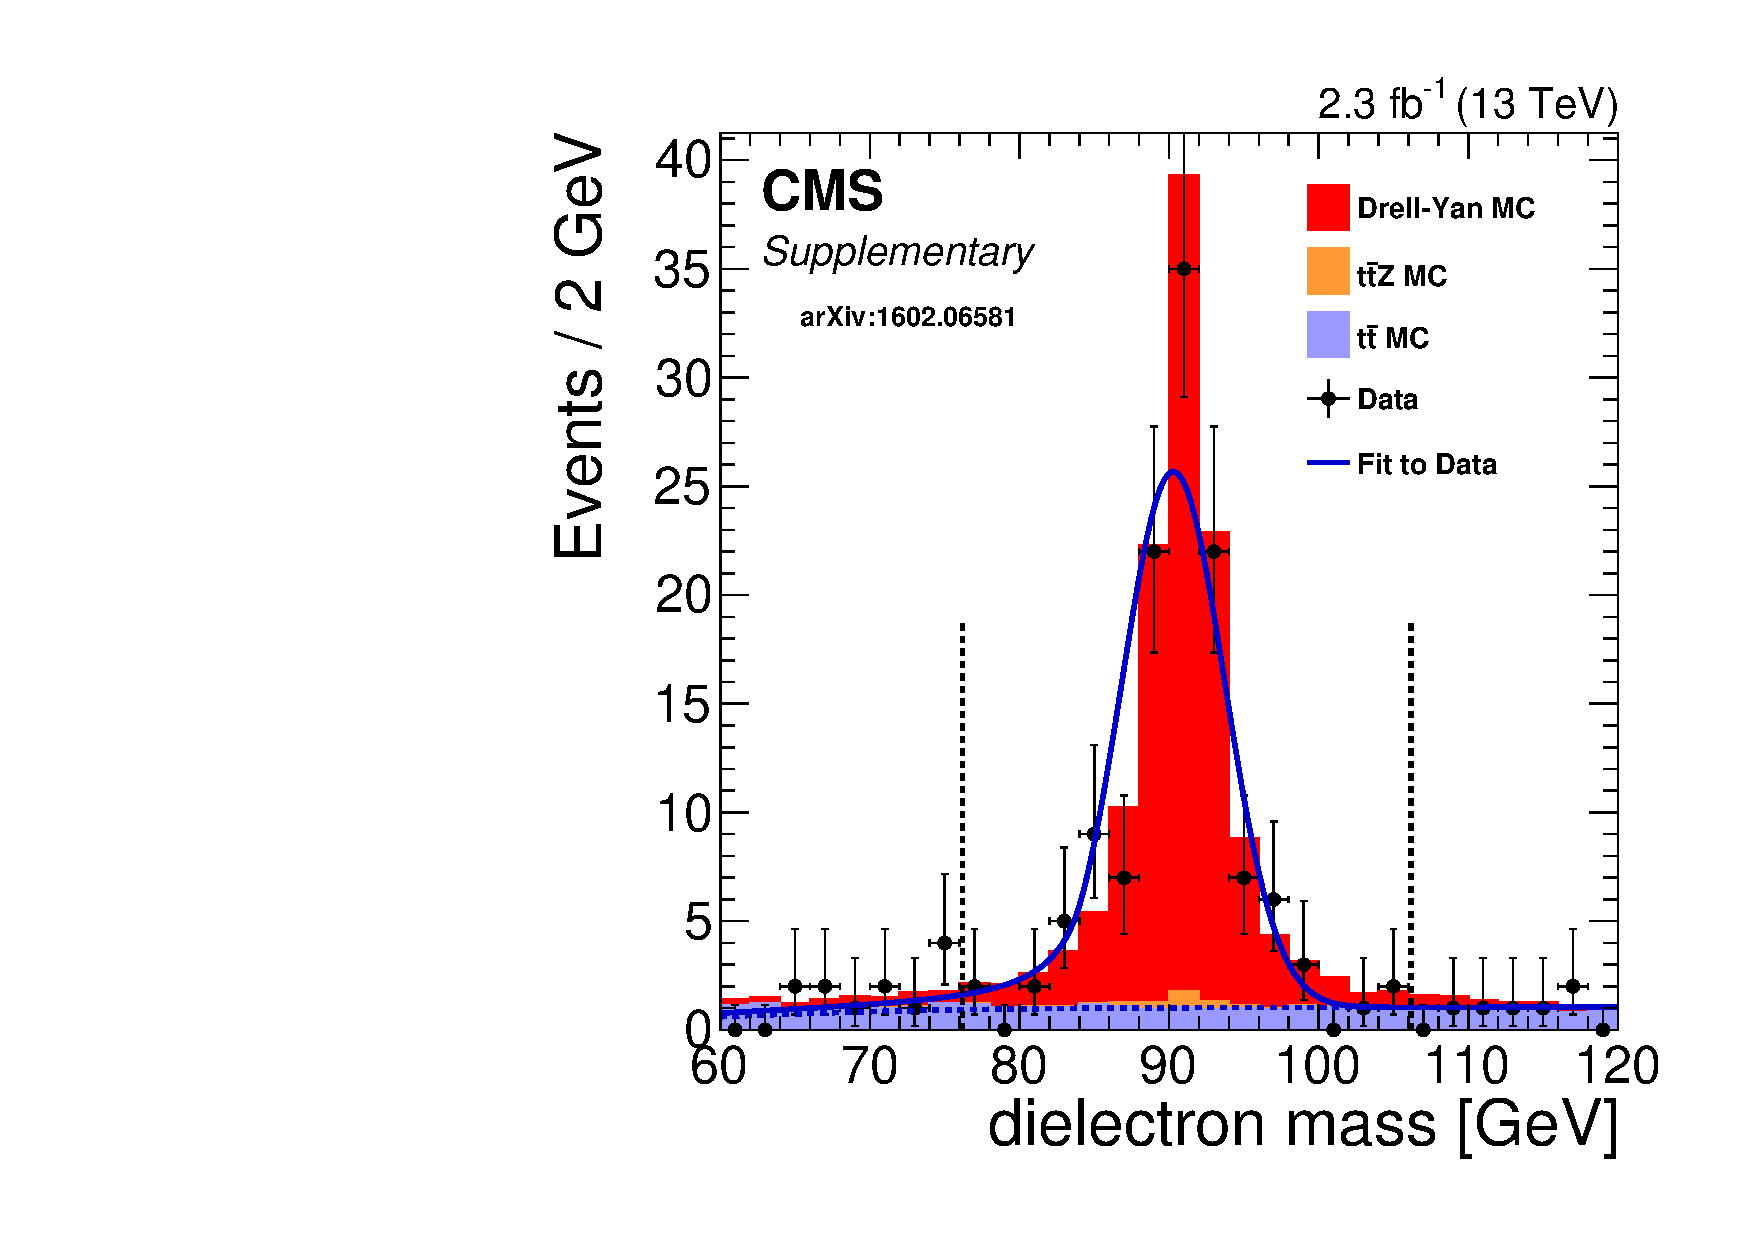
\includegraphics[width=0.48\textwidth]{ee_nJ-1_bJ-1_kin-1.pdf}
  \caption{
    The dimuon (left) and dielectron (right) invariant mass distributions of the $Z\rightarrow\ell^+\ell^-$ control regions. Fit shapes are obtained from a data sample with baseline selection, except for a loosening of the selection on the number of jets to 2. These shapes are then fixed and fit to the baseline selection as shown.   }
\end{figure}

\begin{figure}[htb]
  \centering
  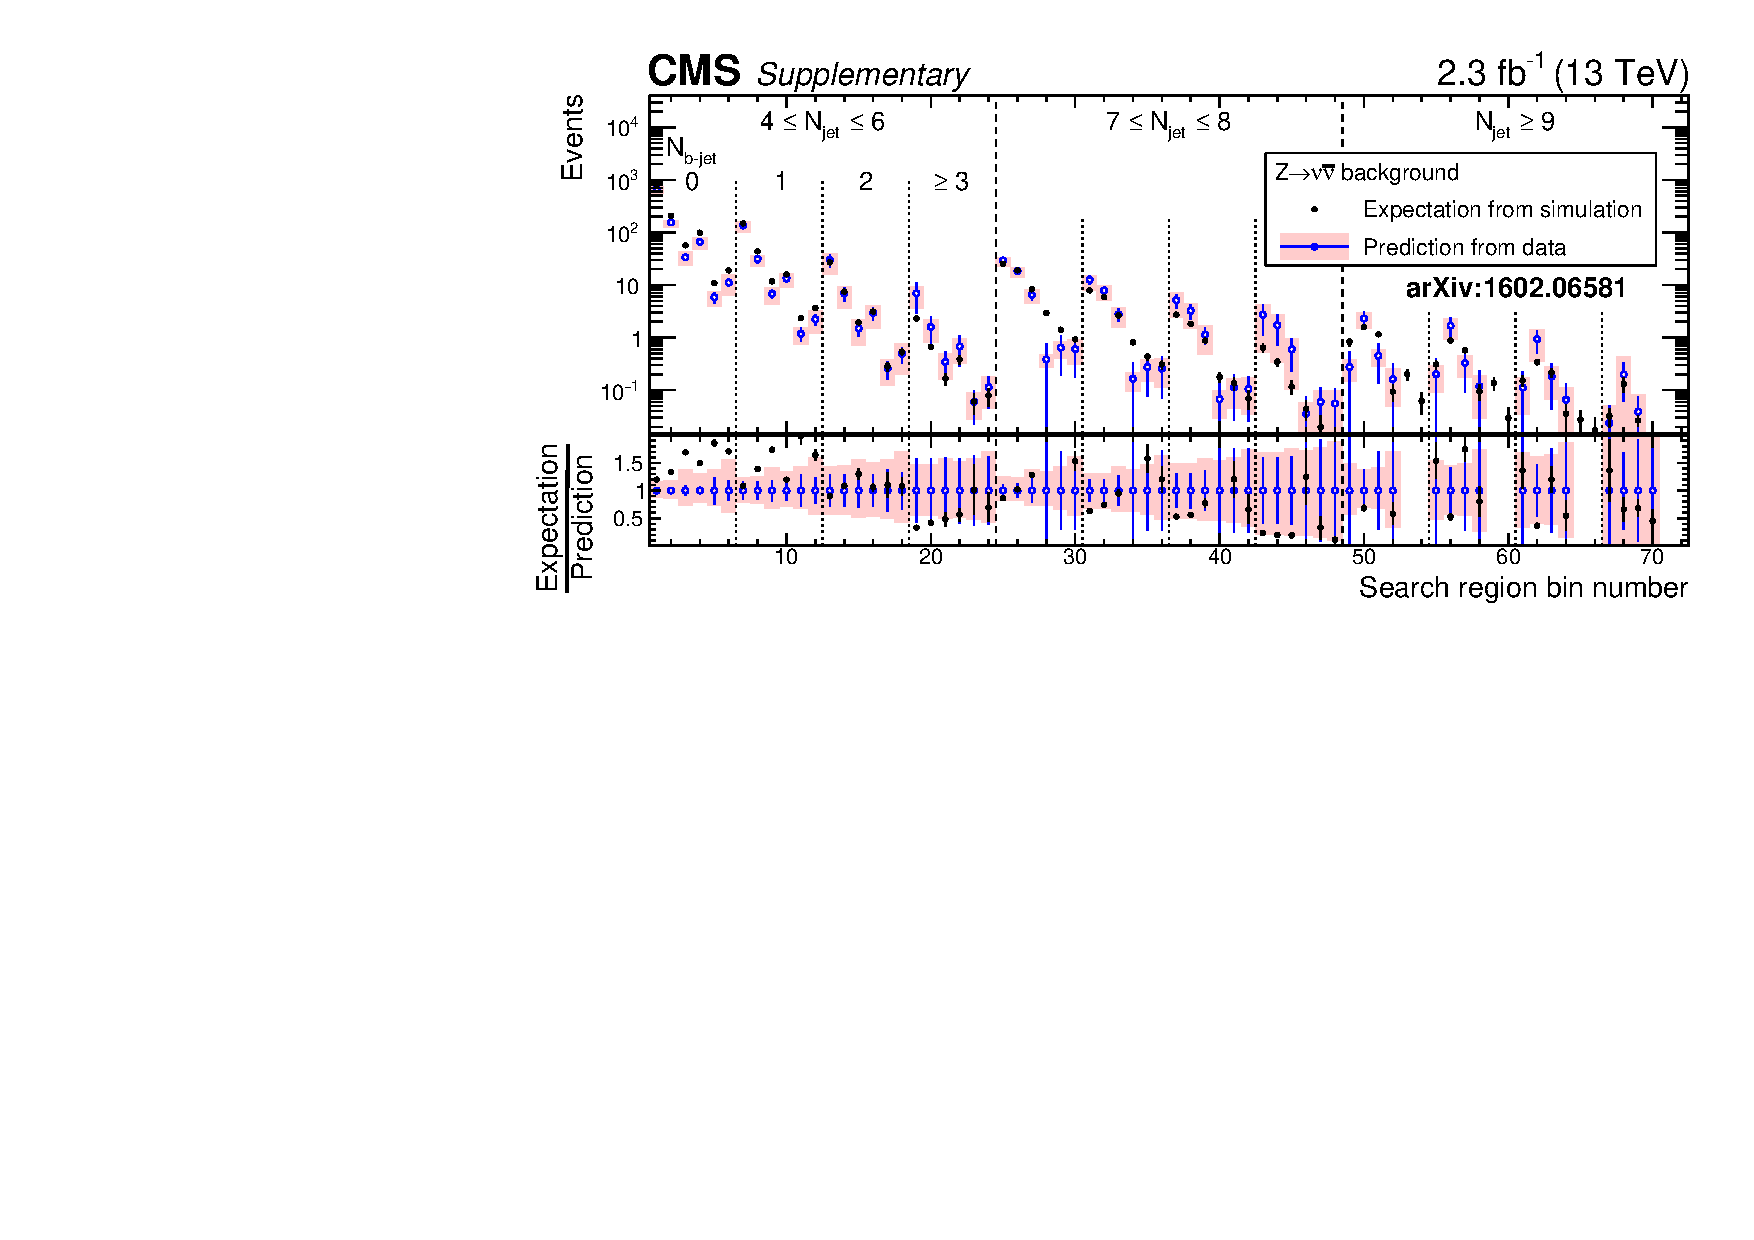
\includegraphics[width=0.9\textwidth]{ZinvBGpred_w_ratio.pdf}
  \caption{
    Predicted $(Z\rightarrow\nu\bar{\nu})+\mathrm{jets}$ yields in the full 72-bin search space, from $\gamma+\mathrm{jets}$ data (for 0 b-tagged jets) combined with the extrapolation factors from $(Z\rightarrow\ell^+\ell^-)+\mathrm{jets}$ (for at least 1 b-tagged jet). Statistical (blue error bars) and systematic (pink shaded) uncertainties are plotted separately, and for comparison the expectation from simulation is overlaid as the black points with (statistical) error bars.   }
\end{figure}

\begin{figure}[htb]
  \centering
  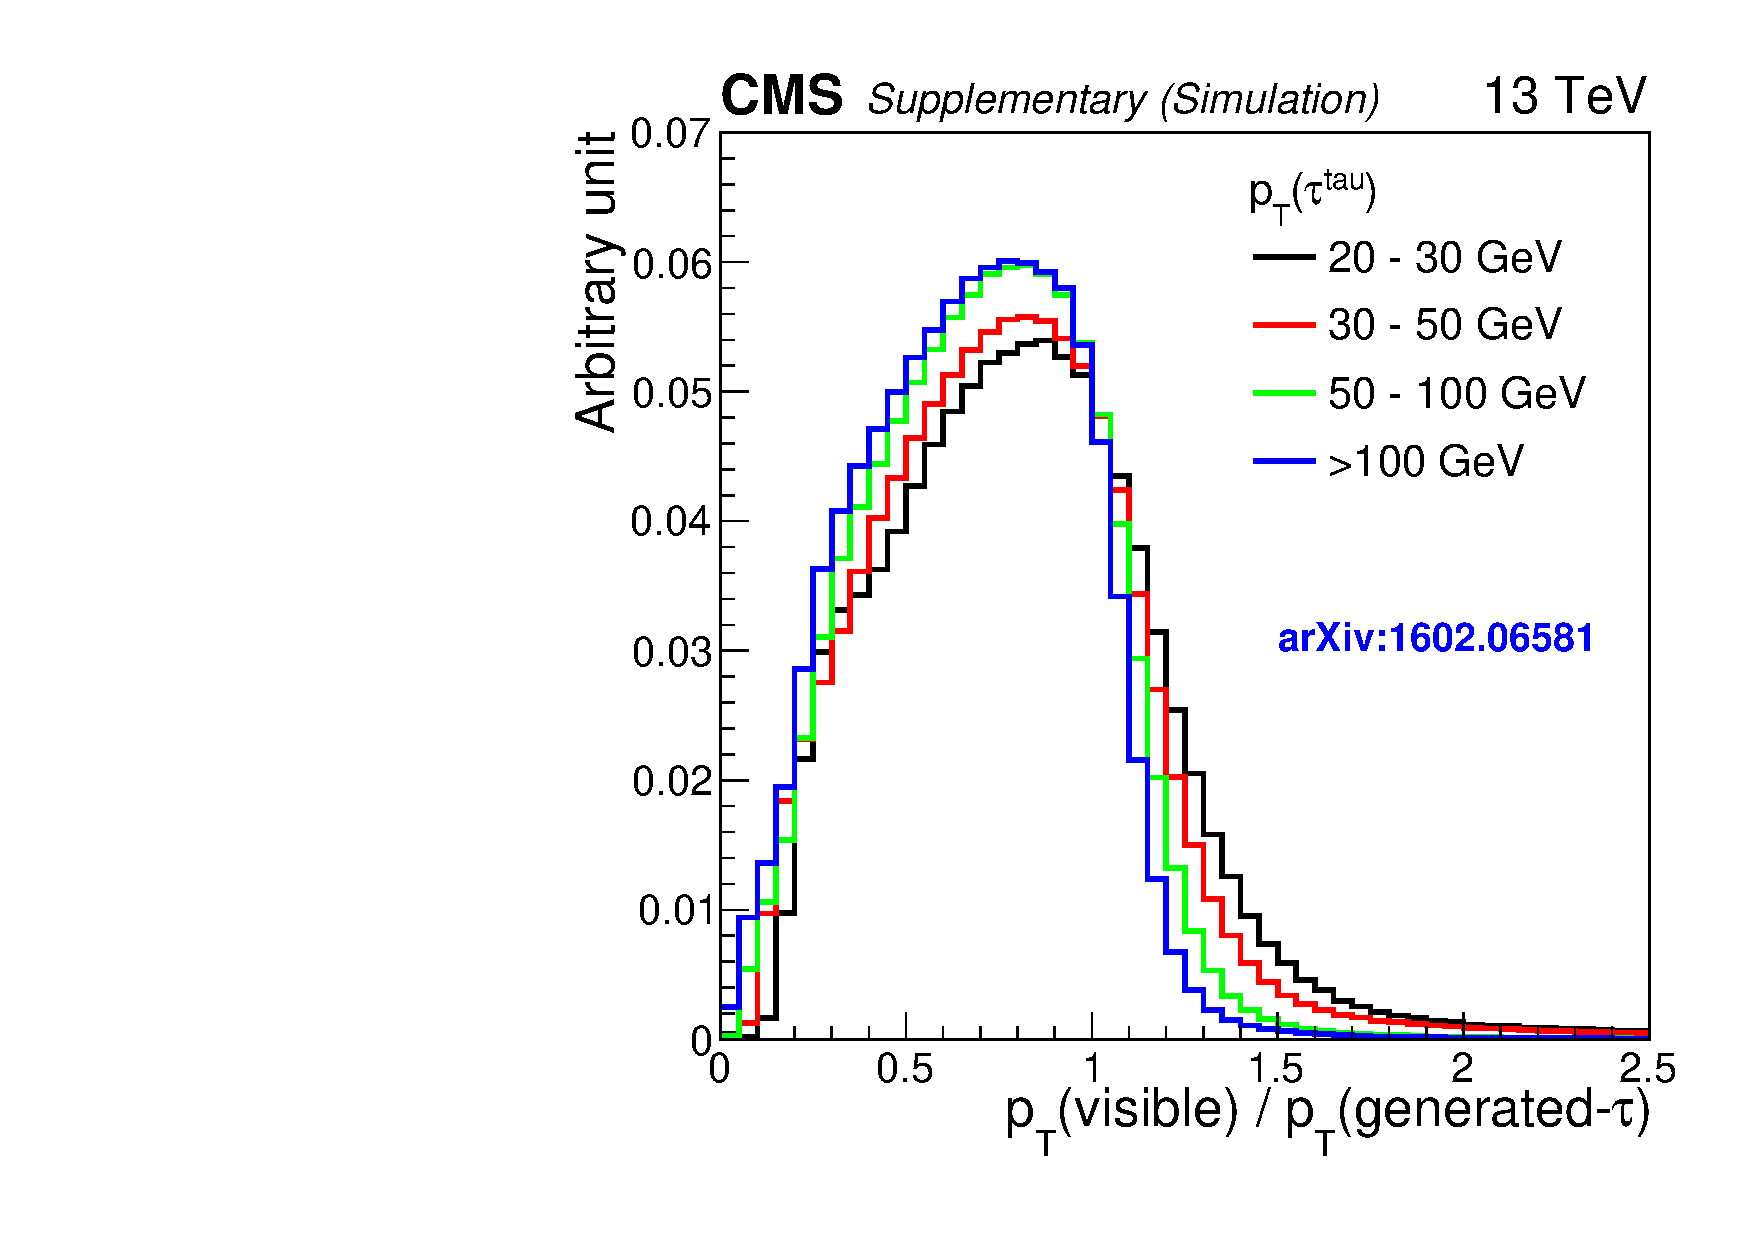
\includegraphics[width=0.9\textwidth]{Plot_TauTemplate_TTbar_Wjets.pdf}
  \caption{
    The $\tau_{h}$ response templates: the distribution of $\frac{p_{\rm T,\;\tau_{h-\mathrm{reco}}}}{p_{\rm T,\;\tau_{h-\mathrm{gen}}}}$ in intervals of $p_{\rm T,\;\tau_{h-\mathrm{gen}}}$, as determined from simulated \ttbar and W+jets events. 
  }
\end{figure}

\begin{figure}[htb]
  \centering
  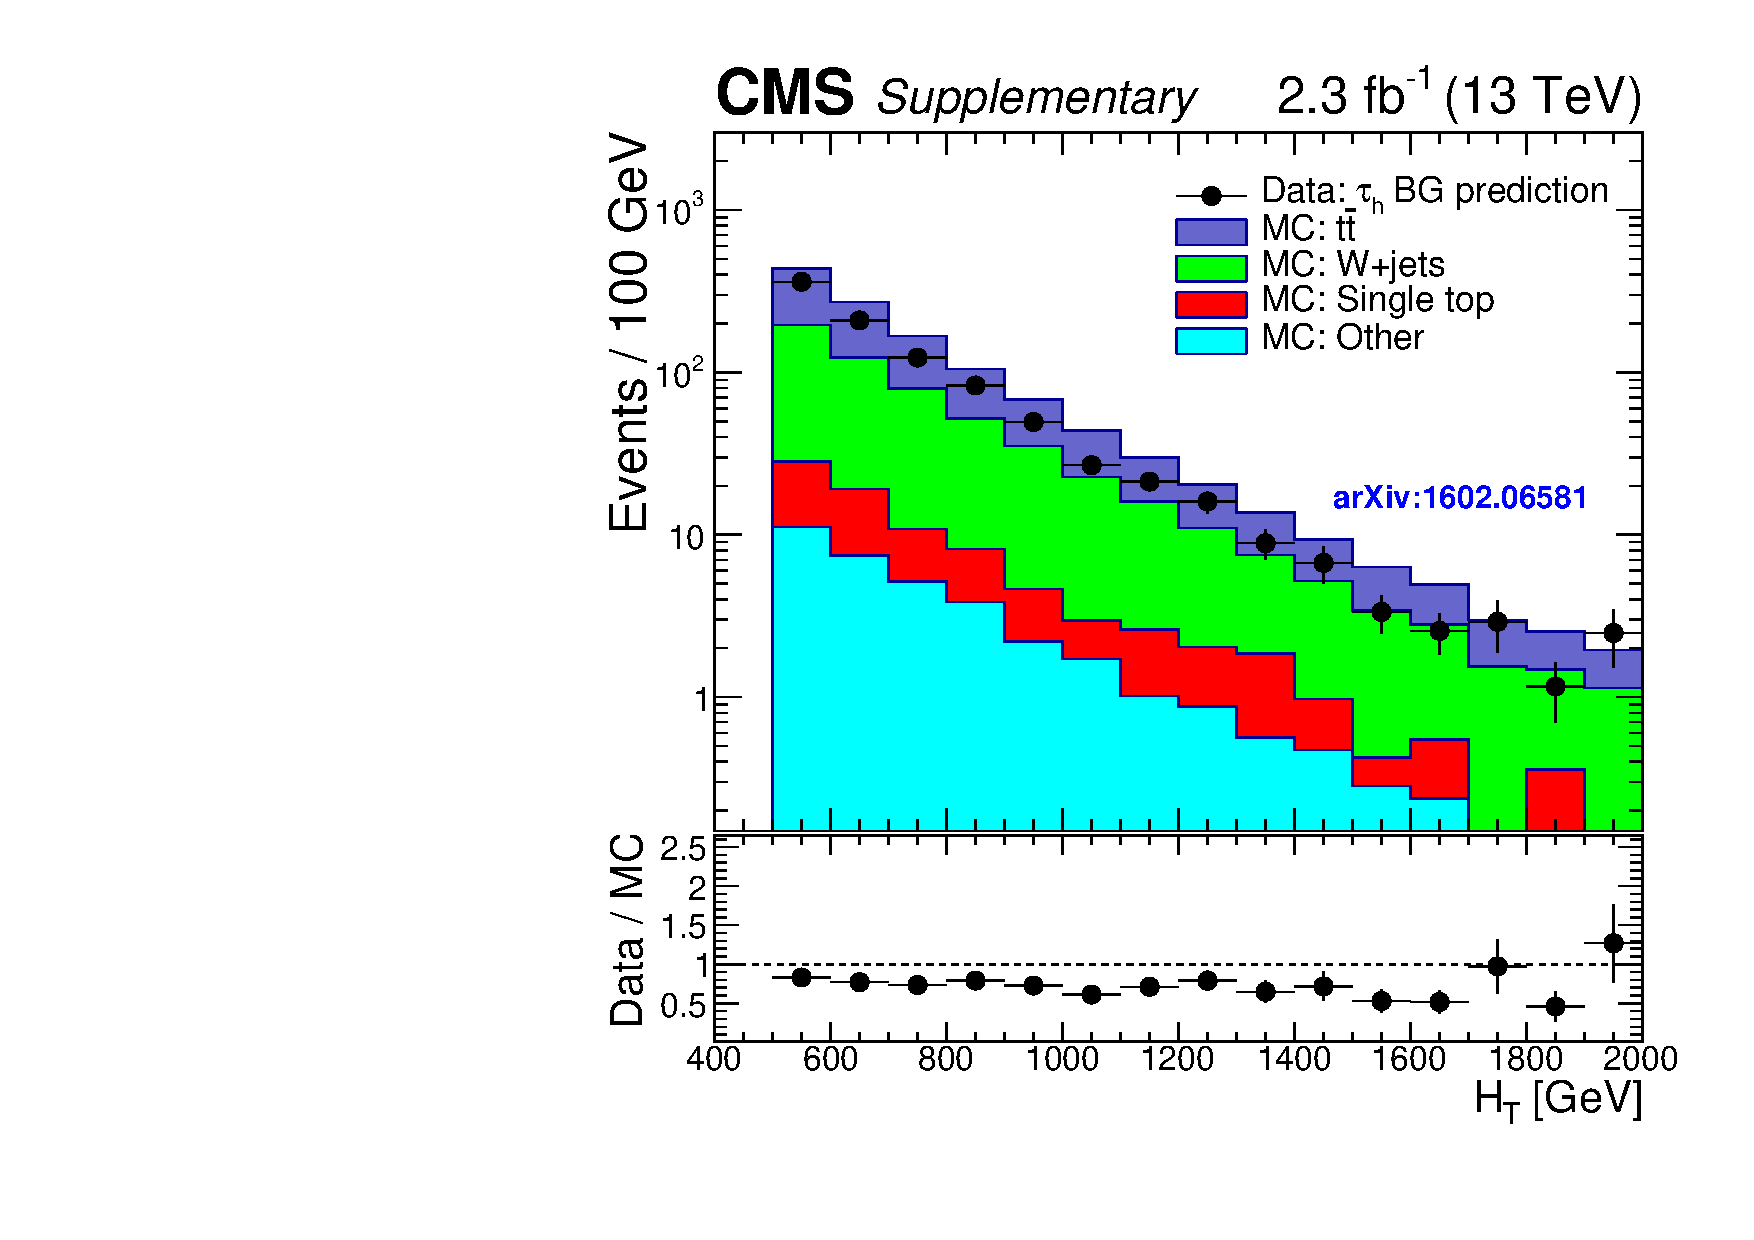
\includegraphics[width=0.49\textwidth]{DataPreVsMCExp_hadtau_HT_delphi_SingleMuon_Plot.pdf}
  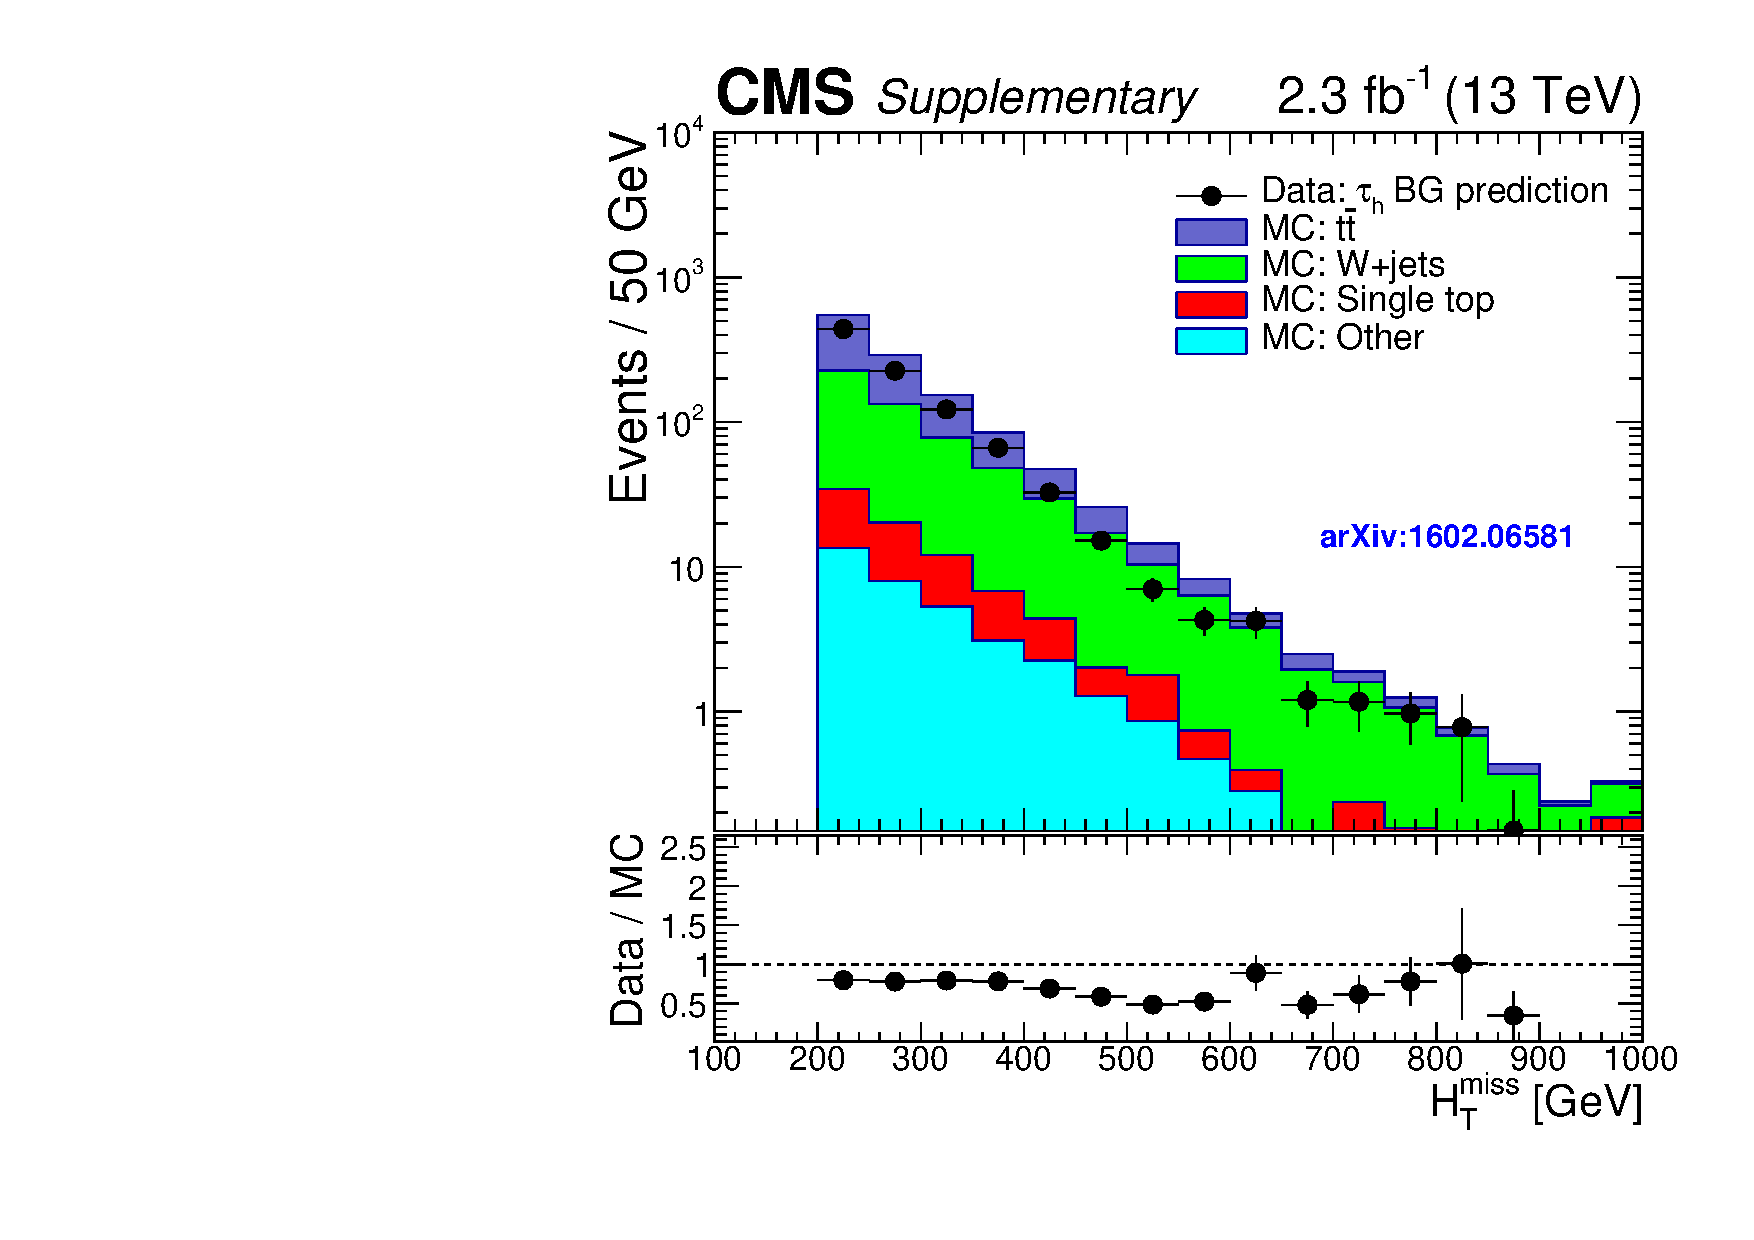
\includegraphics[width=0.49\textwidth]{DataPreVsMCExp_hadtau_MHT_delphi_SingleMuon_Plot.pdf} \\
  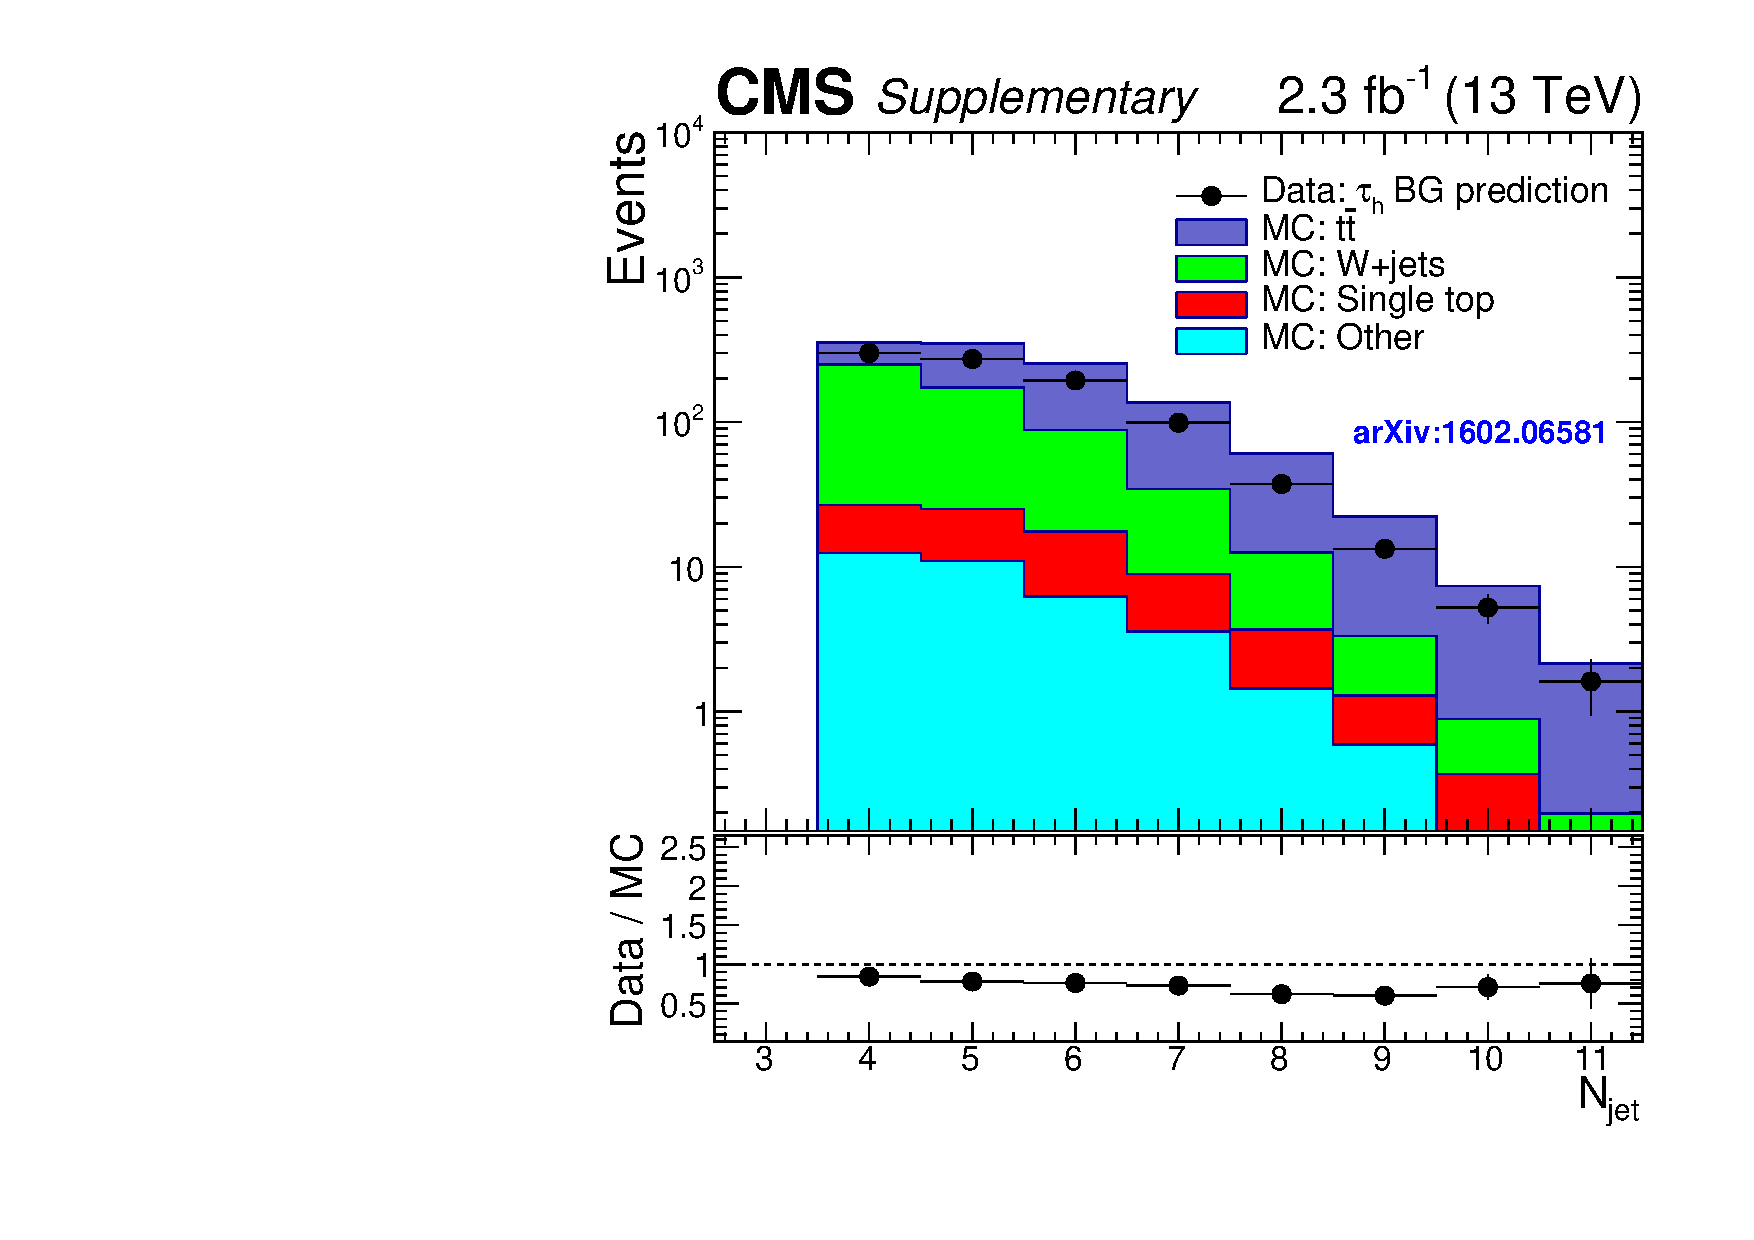
\includegraphics[width=0.49\textwidth]{DataPreVsMCExp_hadtau_NJet_delphi_SingleMuon_Plot.pdf}
  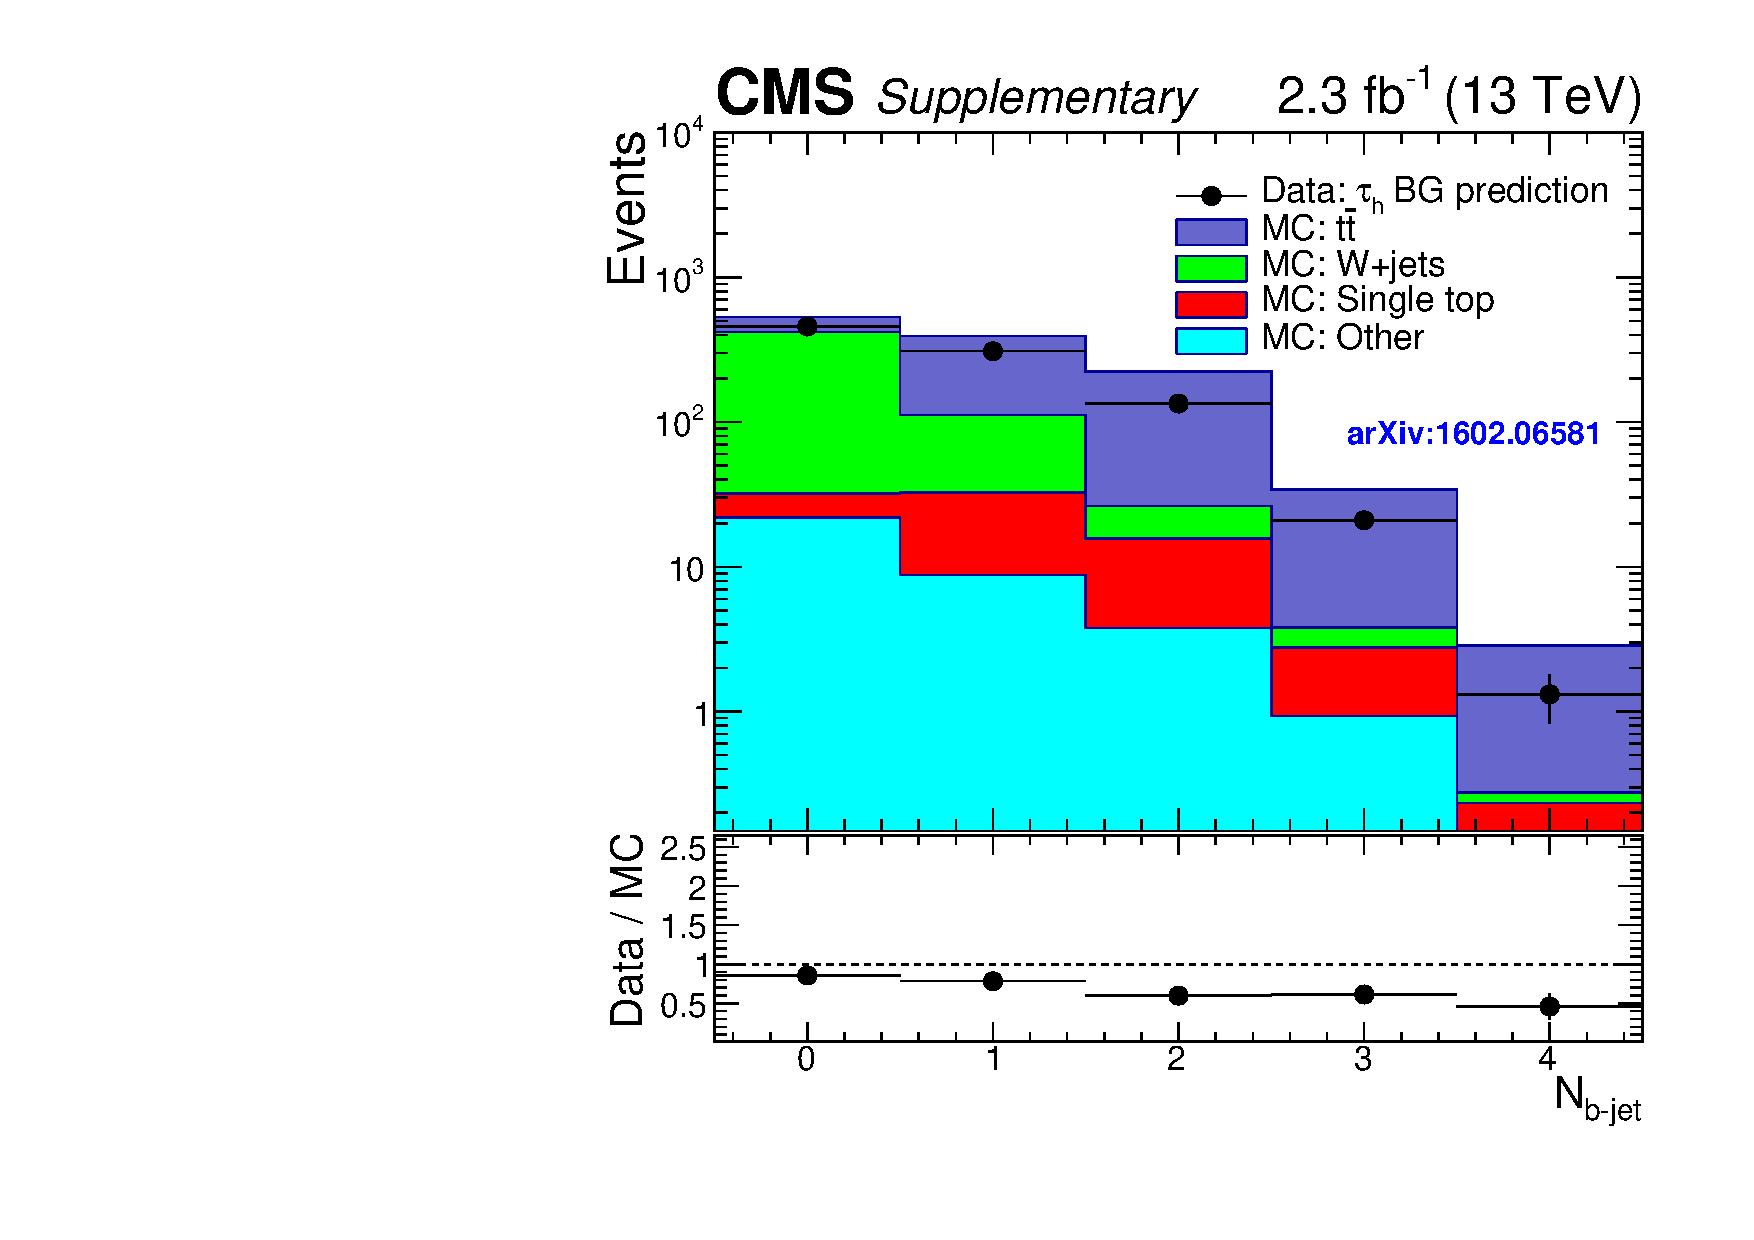
\includegraphics[width=0.49\textwidth]{DataPreVsMCExp_hadtau_NBtag_delphi_SingleMuon_Plot.pdf}
  \caption{
    Clockwise from top-left, distributions of $H_{\rm T}$, $H_{\rm T}^{\rm miss}$, the number of b-tagged jets, and the number of jets in $\tau_{h}$ background events as predicted by performing the data driven background-determination procedure on the 2.3 fb$^{-1}$ of data (shaded regions), compared to the $\tau_{h}$ background expectation from simulation (solid points) for the baseline selection. The simulation includes \ttbar, W+jets, single top quark, and other rare SM process events.}
\end{figure}

\begin{figure}[htb]
  \centering
  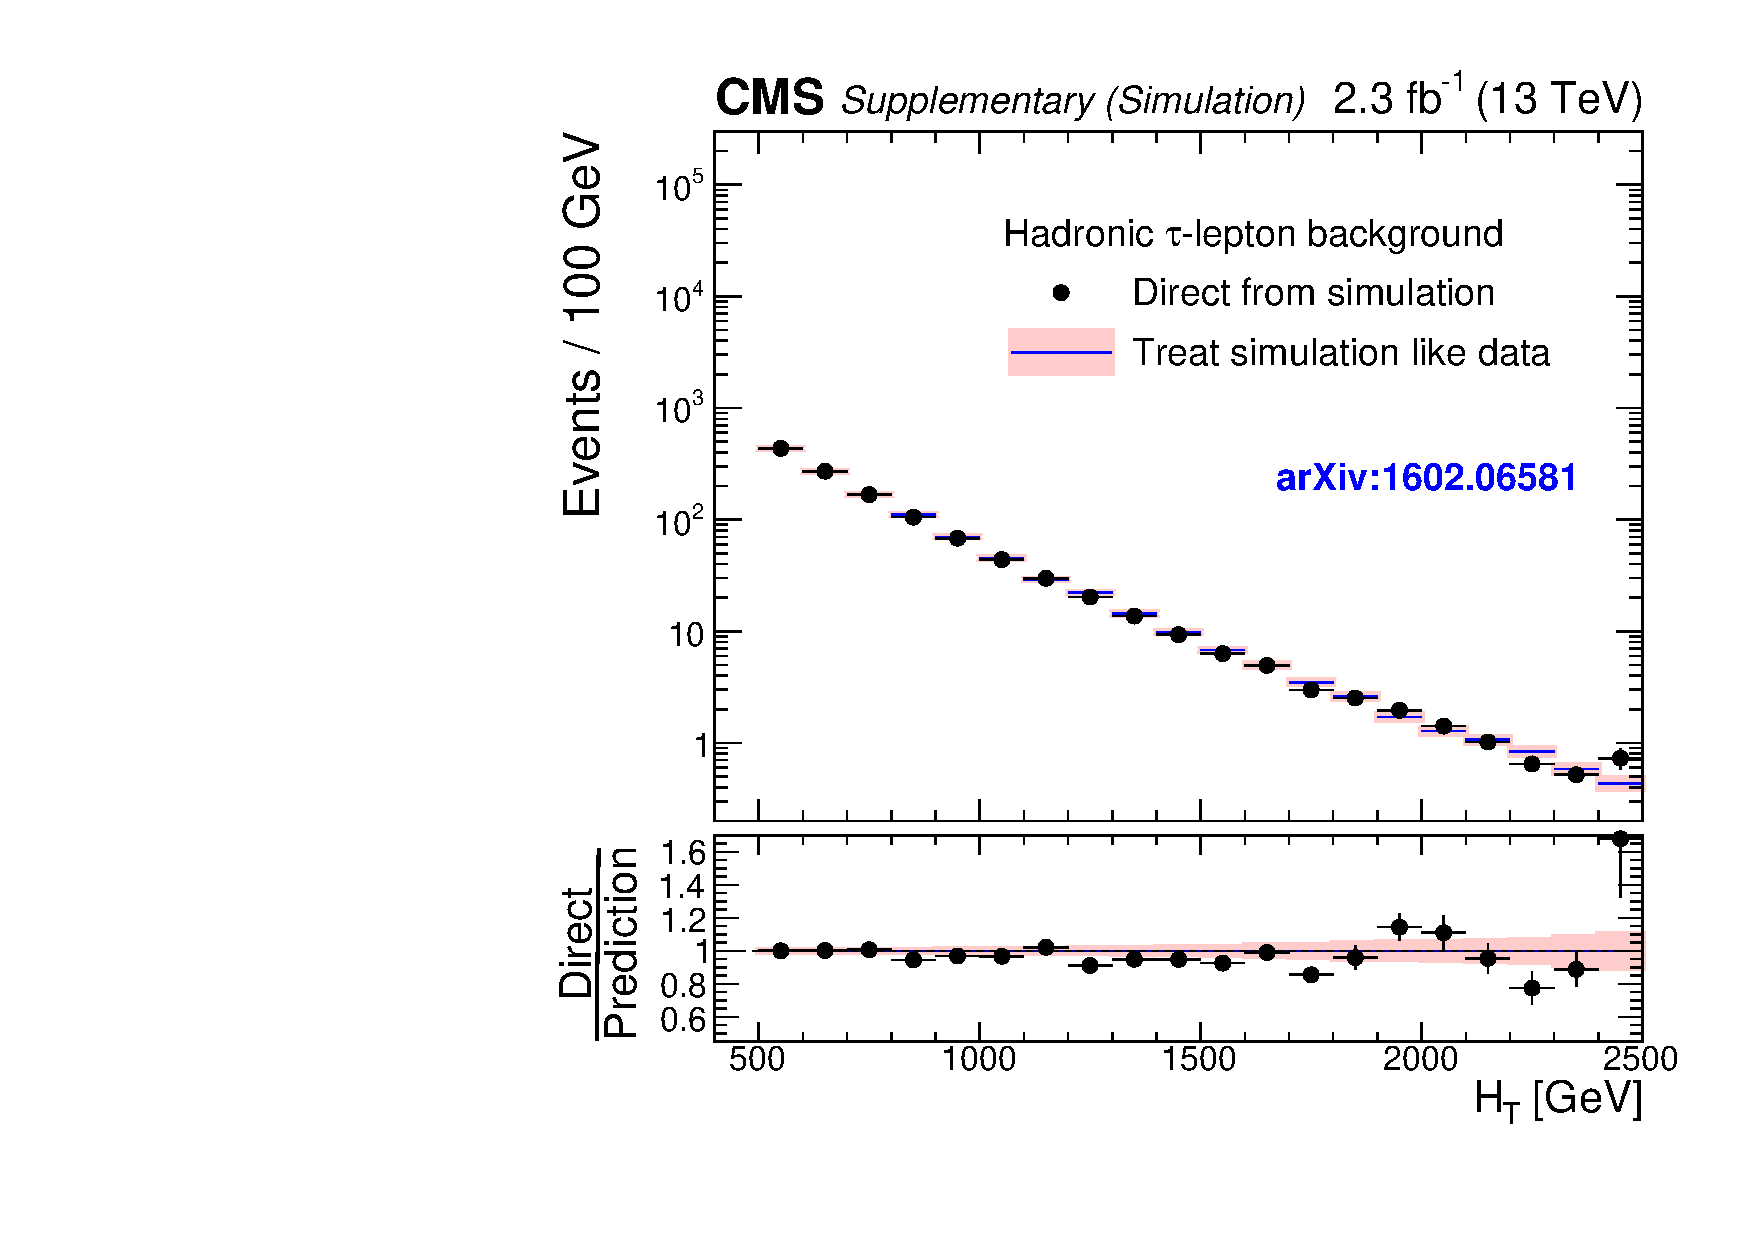
\includegraphics[width=0.49\textwidth]{Closure_HT_delphi_stacked_Elog410_PlusRare_Elog410_PlusRare_Plot.pdf}
  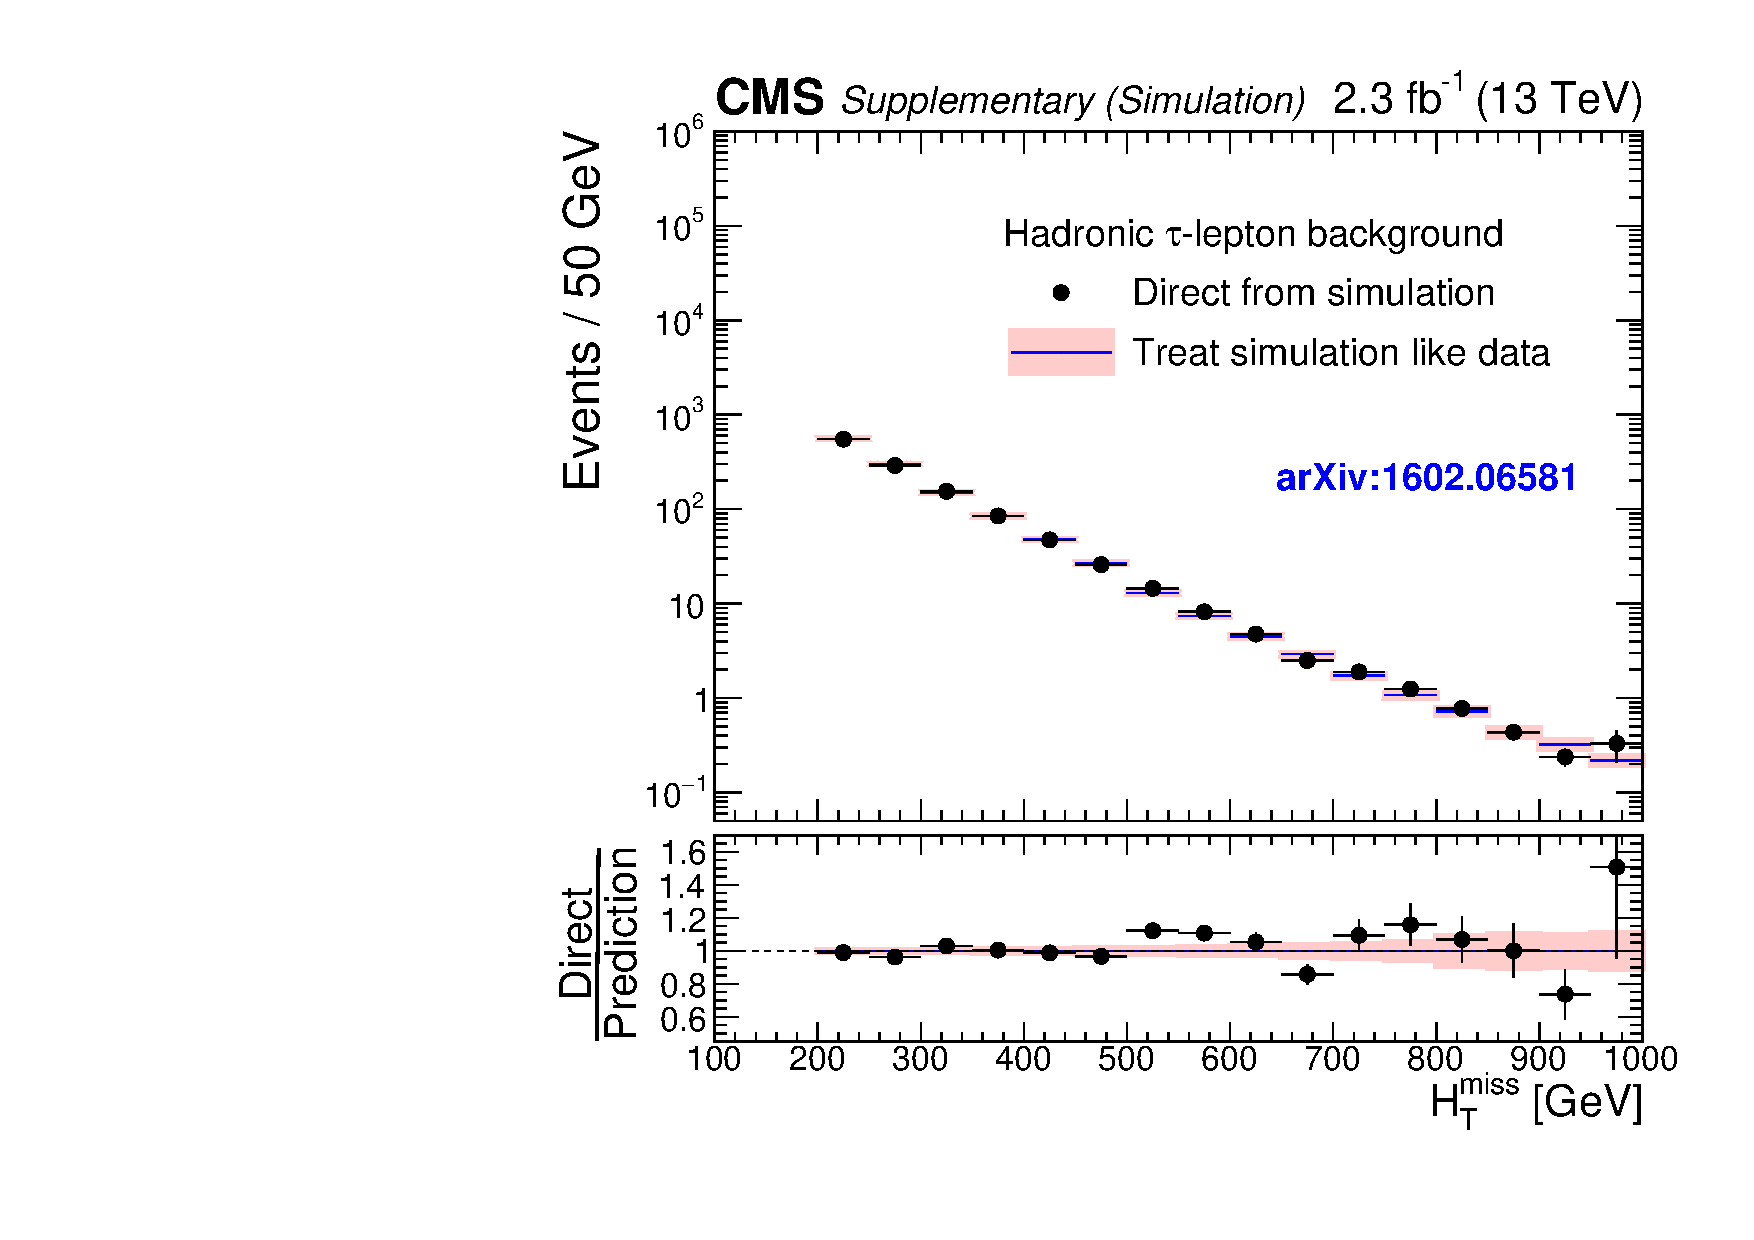
\includegraphics[width=0.49\textwidth]{Closure_MHT_delphi_stacked_Elog410_PlusRare_Elog410_PlusRare_Plot.pdf} \\
  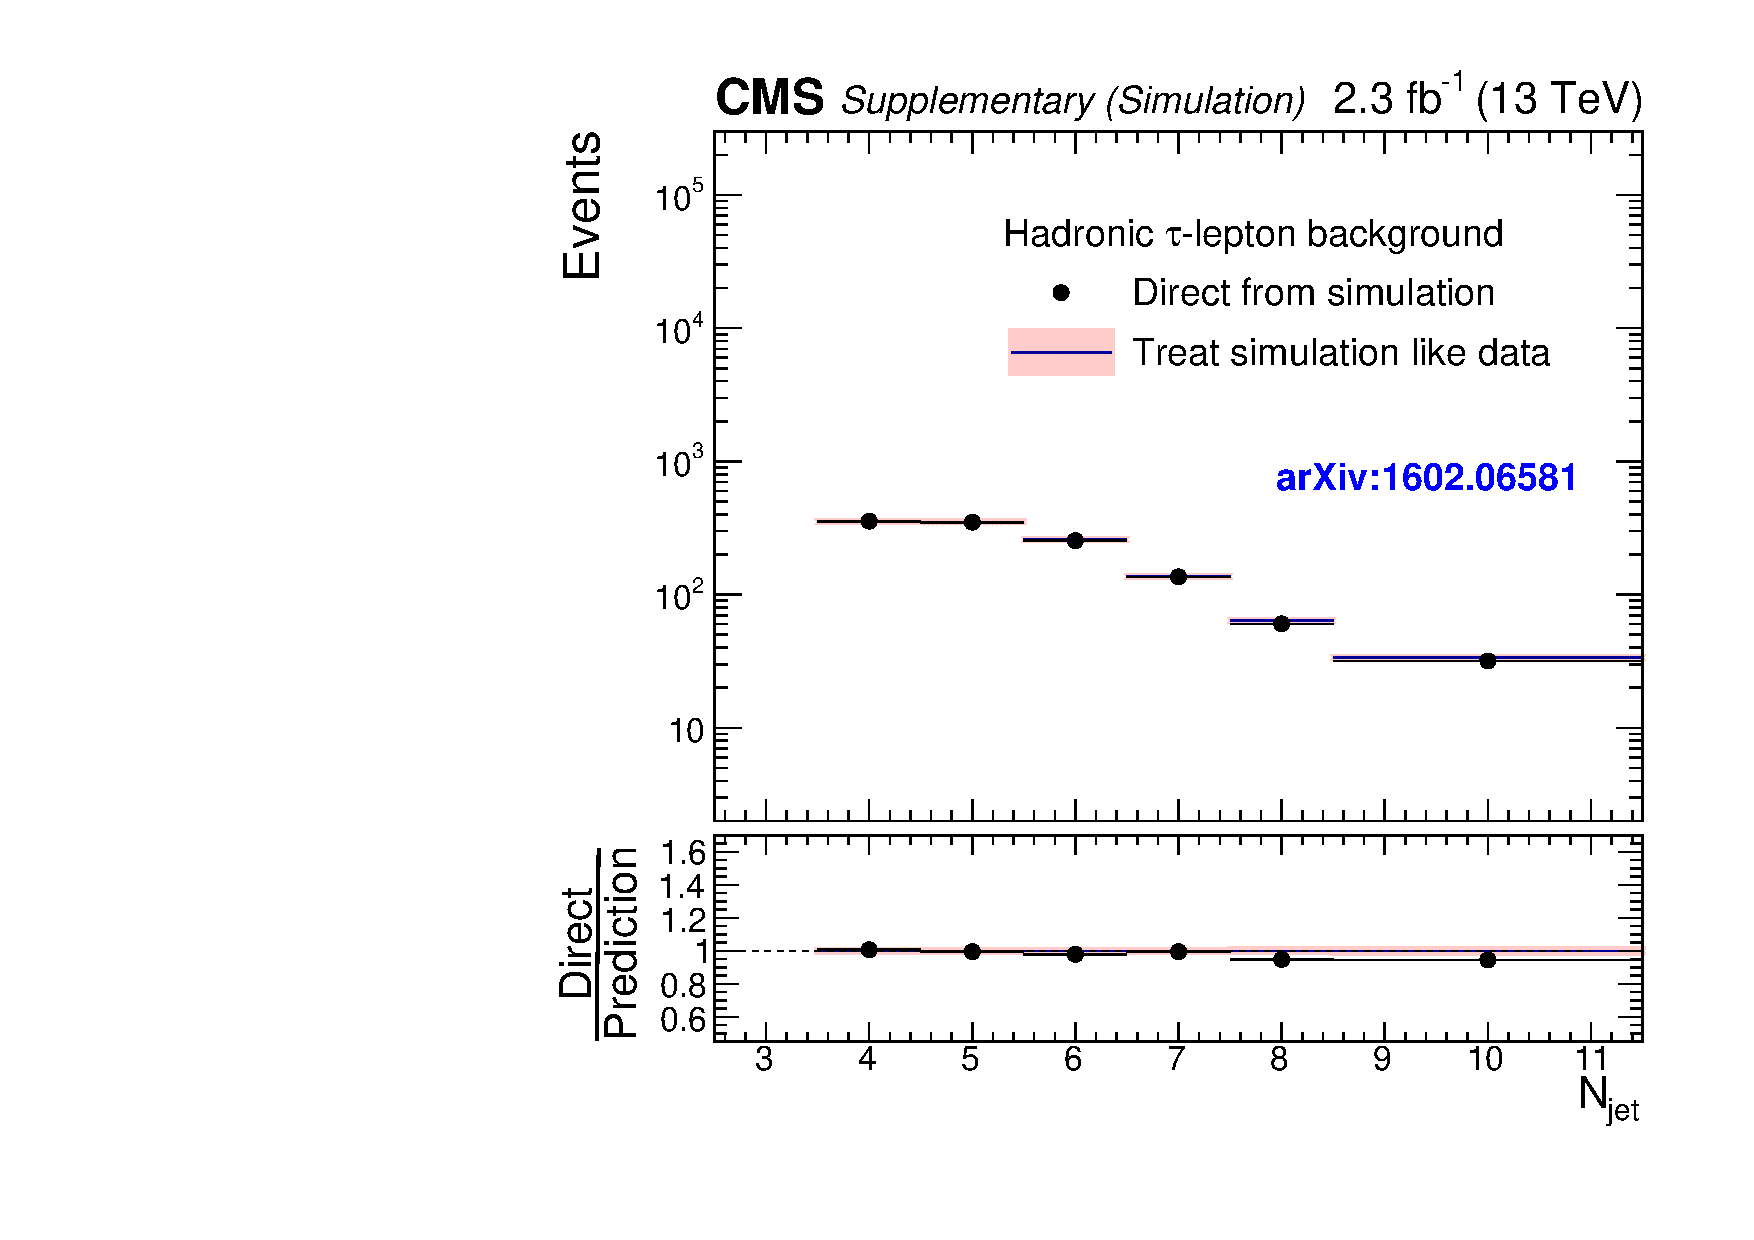
\includegraphics[width=0.49\textwidth]{Closure_NJet_delphi_stacked_Elog410_PlusRare_Elog410_PlusRare_Plot.pdf}
  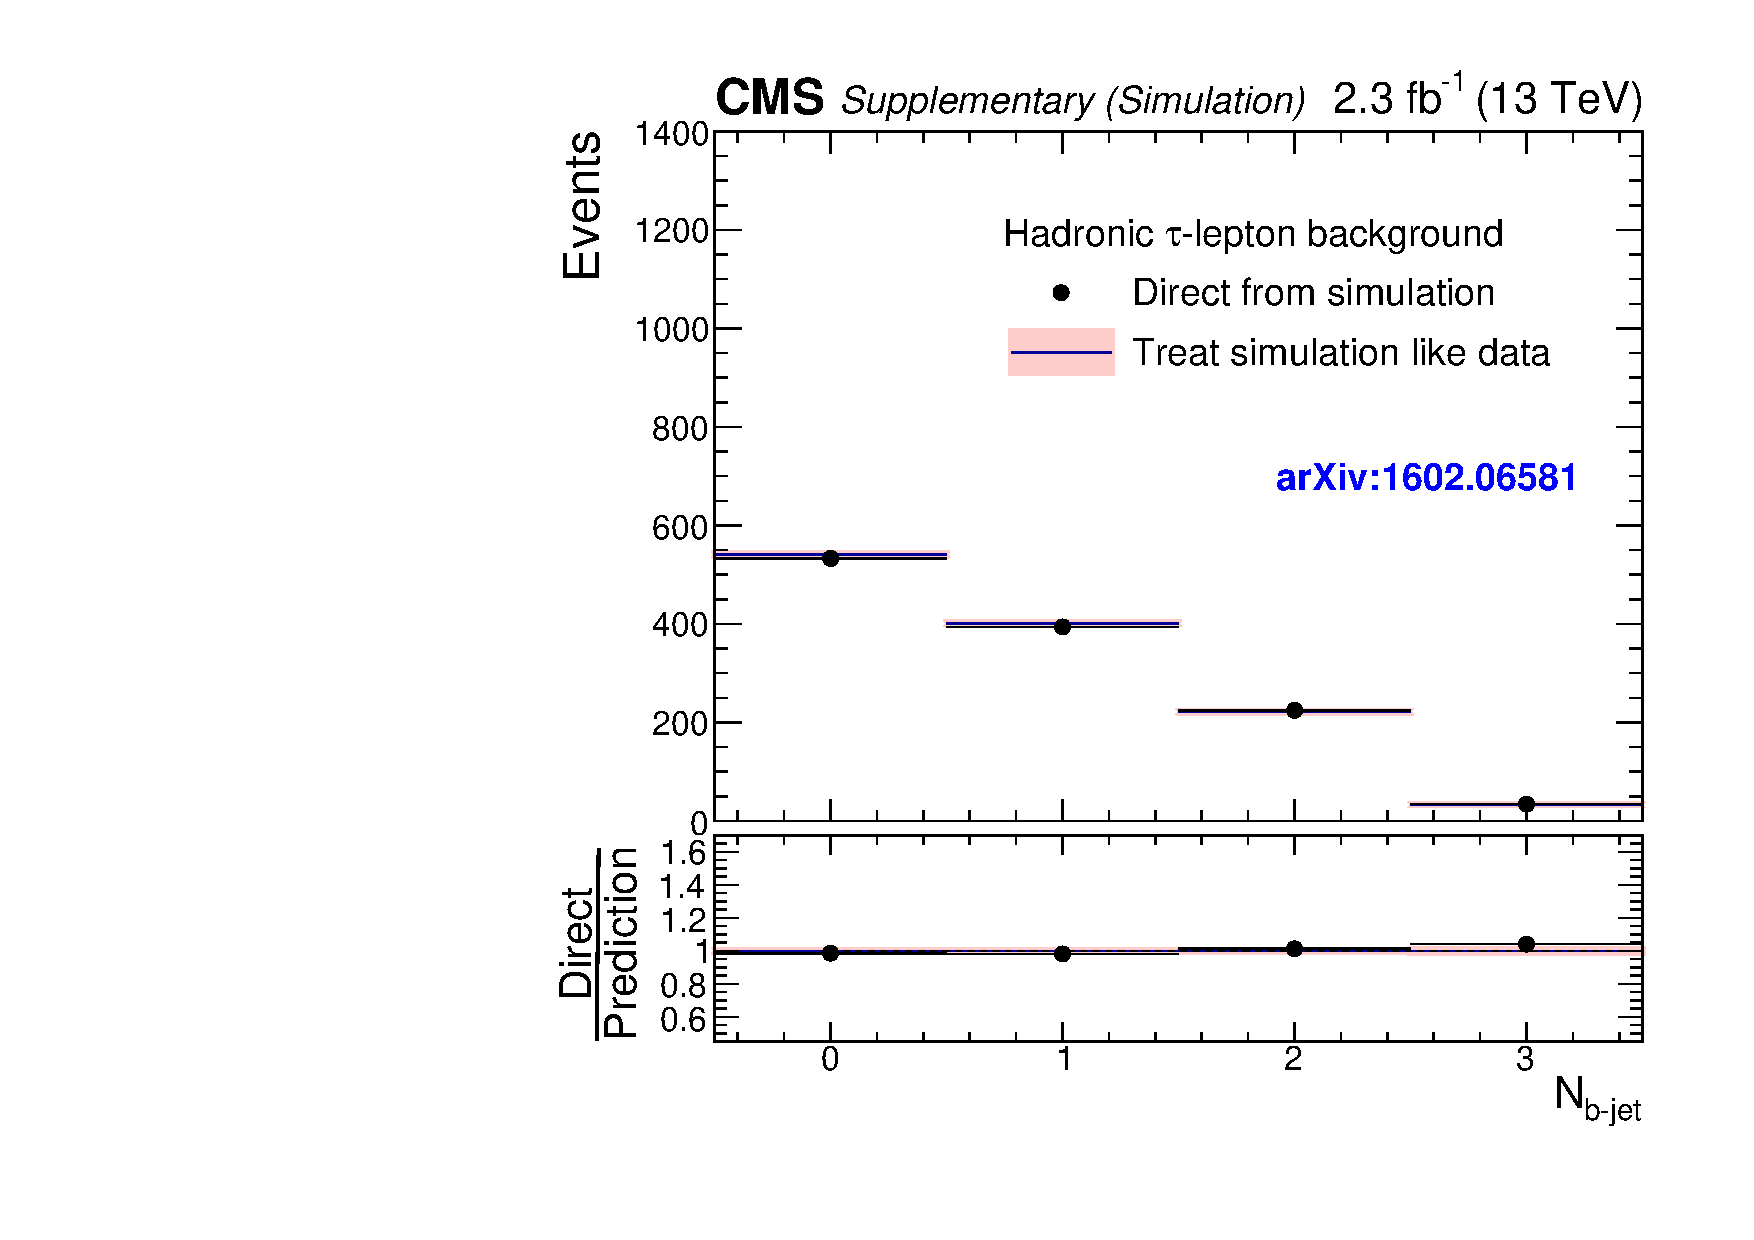
\includegraphics[width=0.49\textwidth]{Closure_NBtag_delphi_stacked_Elog410_PlusRare_Elog410_PlusRare_Plot.pdf}
  \caption{
    Clockwise from top-left, distributions of $H_{\rm T}$, $H_{\rm T}^{\rm miss}$, the number of b-tagged jets, and the number of jets in $\tau_{h}$ background events as predicted directly from simulation (solid points) and as predicted by the data-driven background-determination procedure (shaded regions), for the baseline selection. The simulation simulation includes t$\bar{t}$, W+jets, single-top, Drell-Yan, and other rare SM process events. 
  }
\end{figure}

\clearpage 
\begin{figure}[htb]
  \centering
  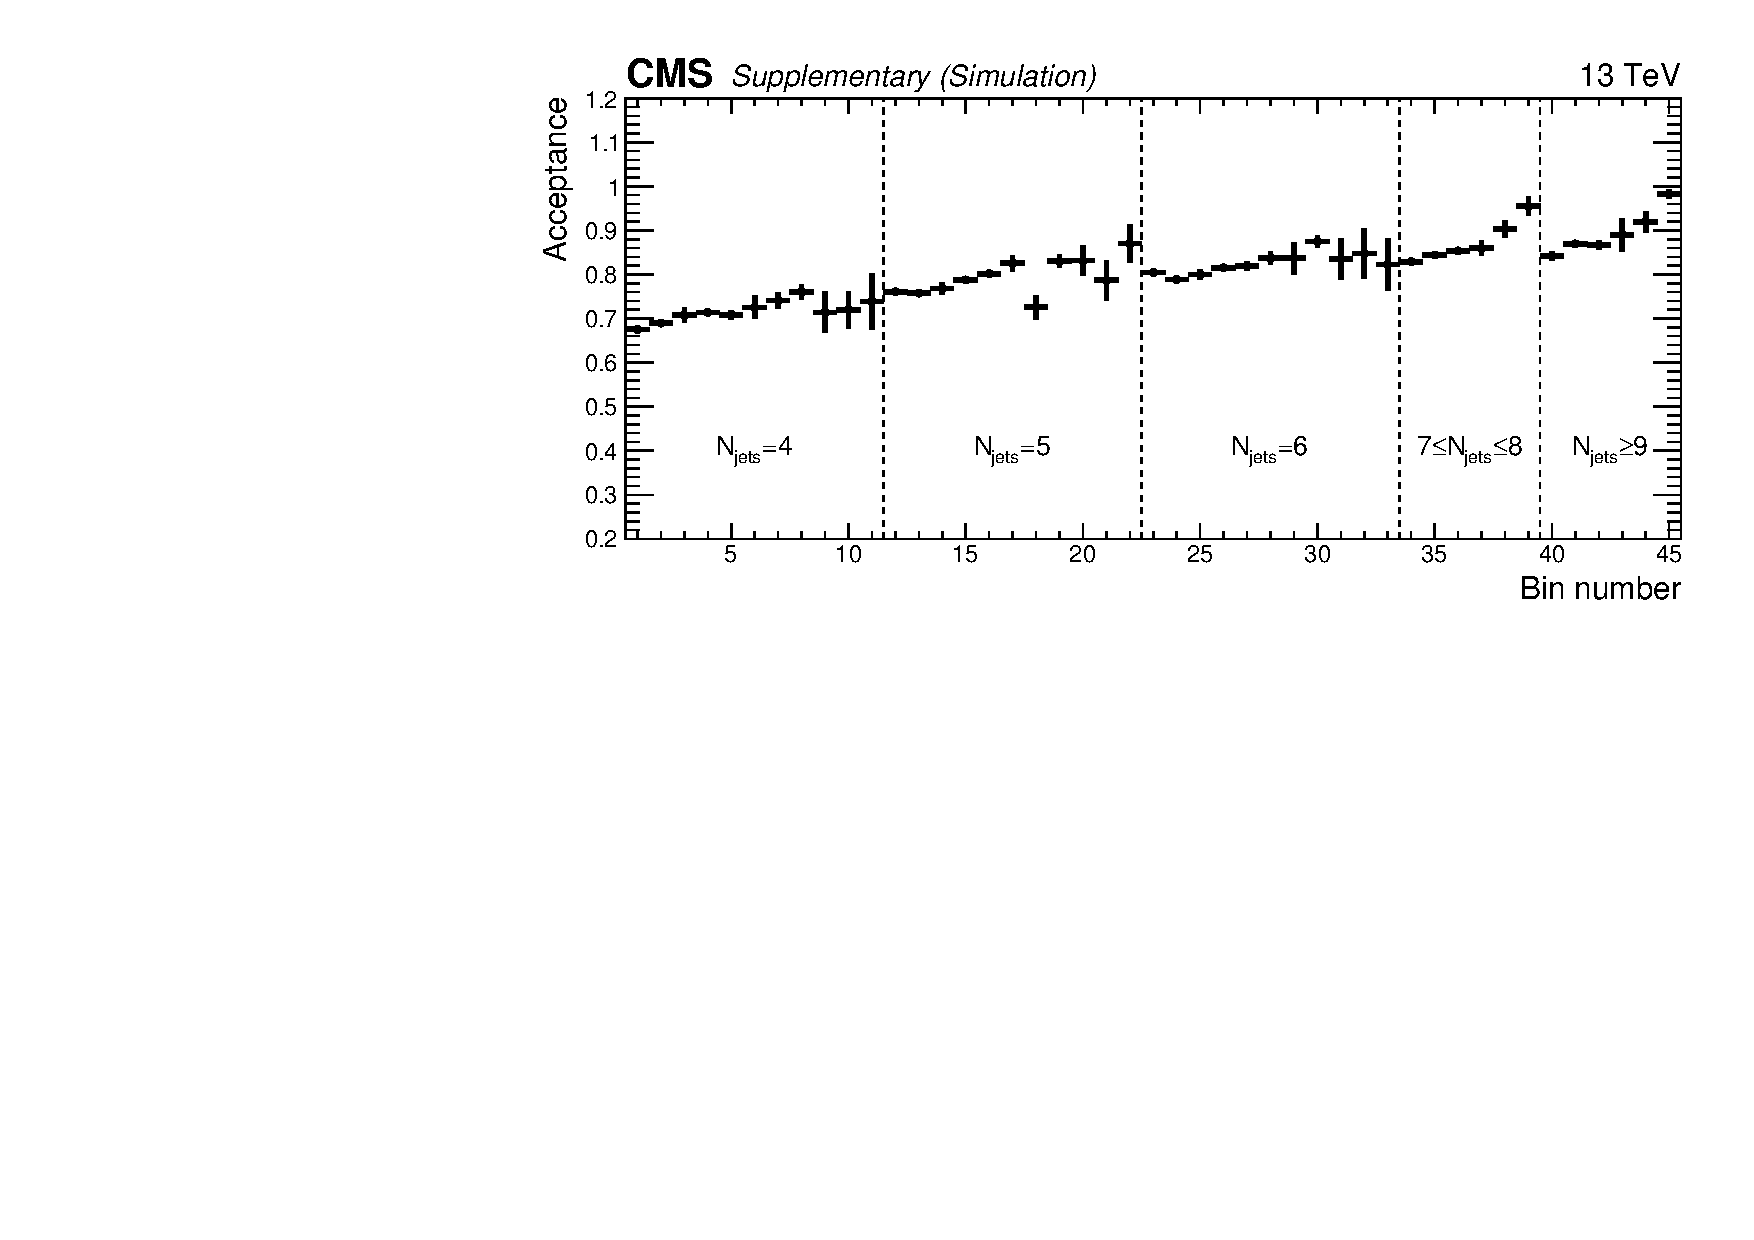
\includegraphics[width=0.9\textwidth]{plot_Acceptance.pdf}
  \caption{
    Acceptance $\epsilon^{\mu}_{Acc}$ of hadronically-decaying $\tau$ leptons for $ p_{T} > 20 $ GeV and $ \eta < 2.1$. The results are shown as a function of $H_{\rm T}^{\rm miss}$,  $H_{\rm T}$, and $N_{\rm jet}$, integrated over the four bins of $N_{\rm b-jet}$ (in total 45 bins).
  }
\end{figure}

\begin{figure}[htb]
  \centering
  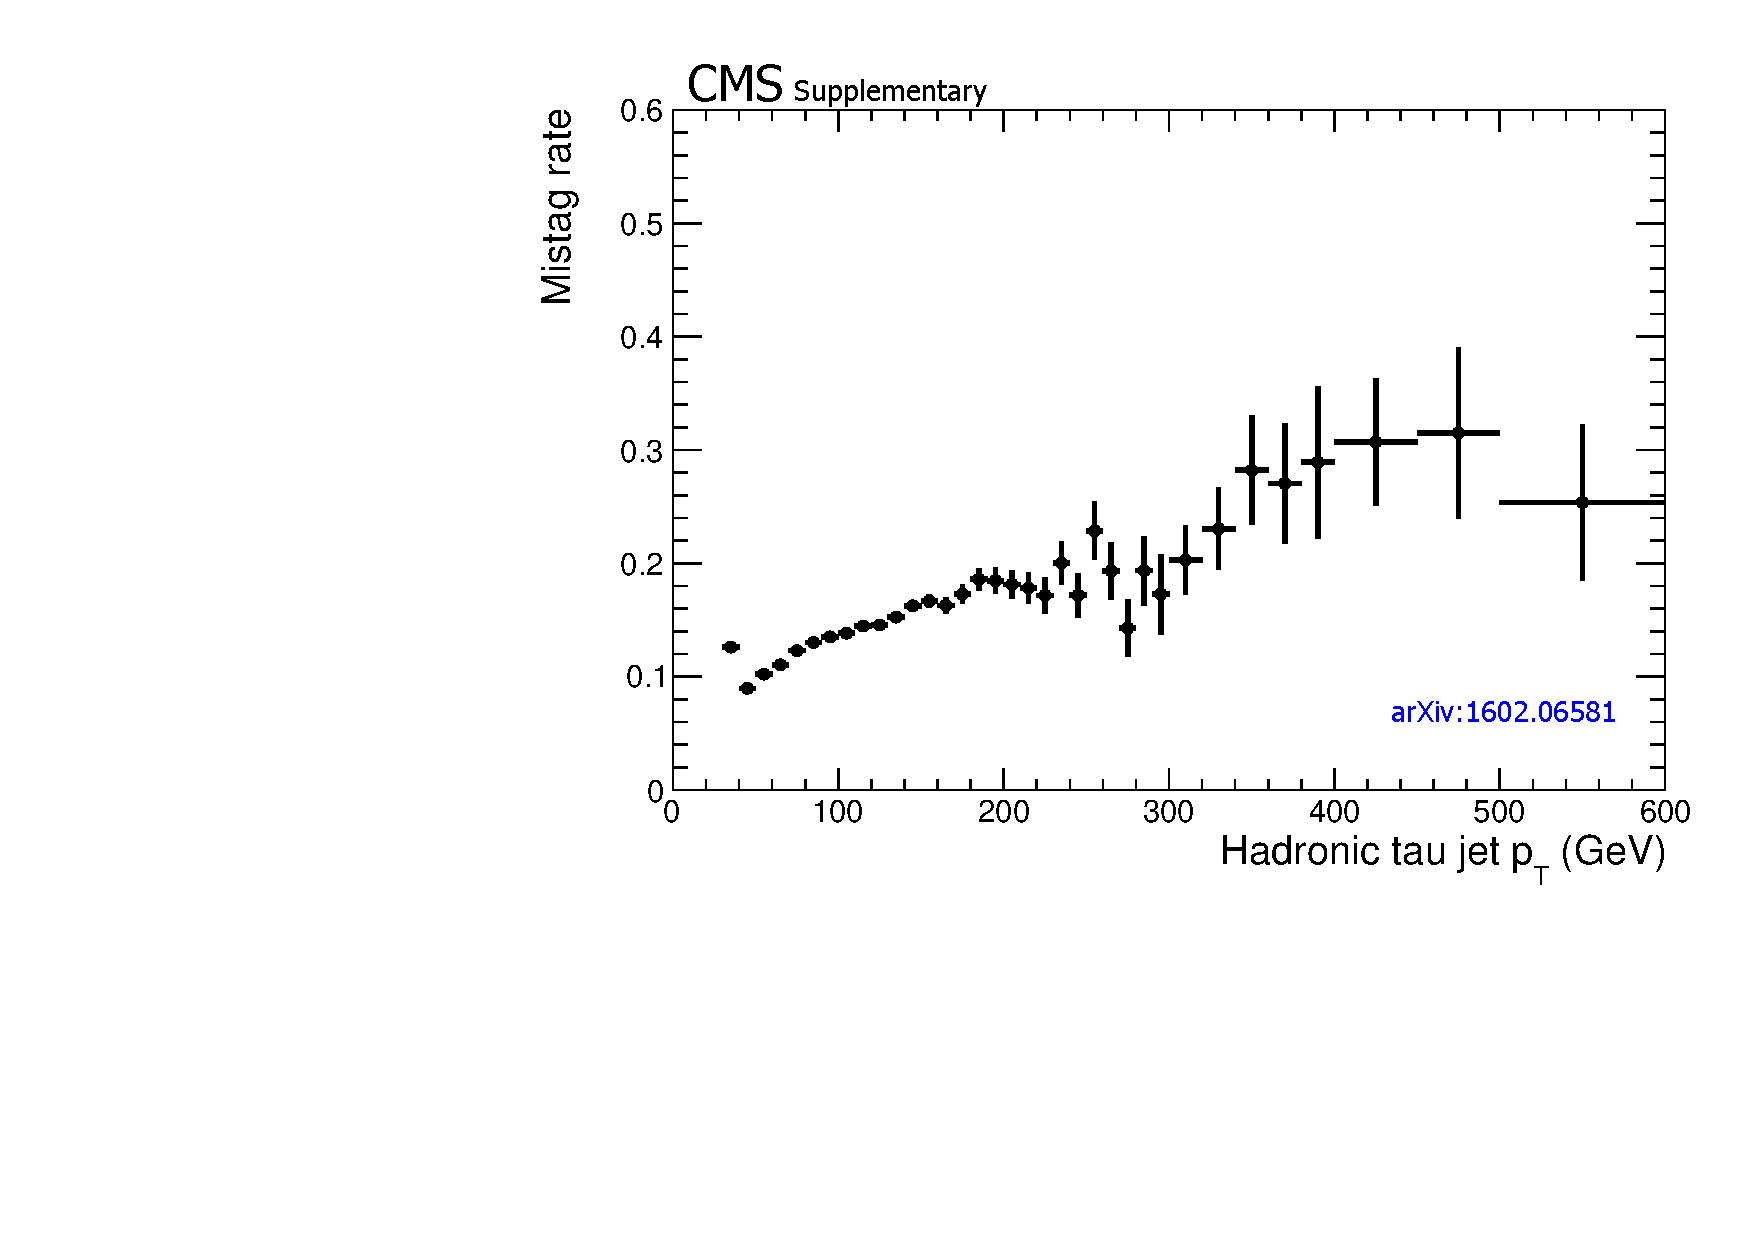
\includegraphics[width=0.9\textwidth]{plot_HadTauBtaggedRate.pdf}
  \caption{
    The mistag rate of $\tau_{h}$ jet as function of transverse momentum.
  }
\end{figure}

\begin{figure}[htb]
  \centering
  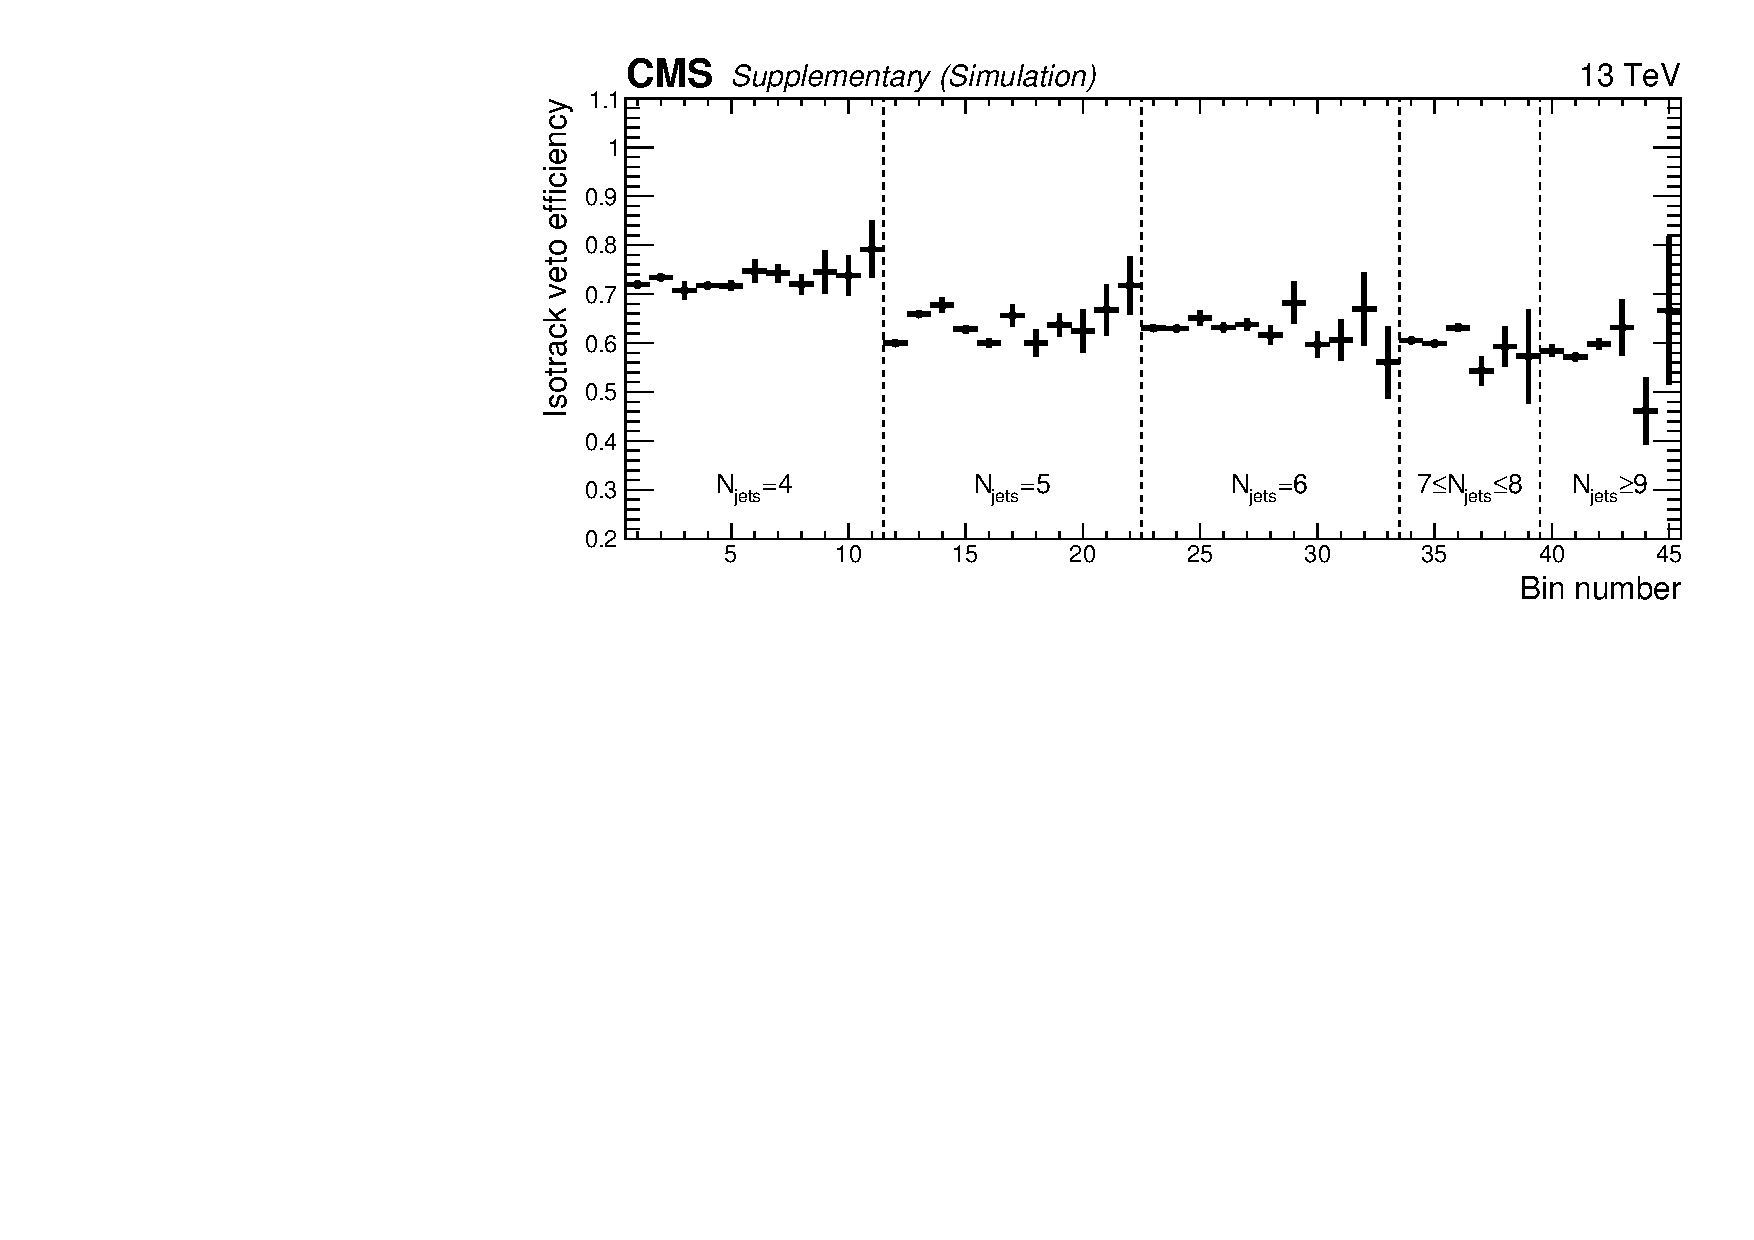
\includegraphics[width=0.9\textwidth]{plot_IsoTrackVetoEfficiencies.pdf}
  \caption{
    The isolated-track veto efficiency $\epsilon_{isotrk}$. The results are shown as a function of $H_{\rm T}^{\rm miss}$, $H_{\rm T}$, and $N_{\rm jet}$, integrated over the four bins of $N_{\rm b-jet}$ (in total 45 bins).
  }
\end{figure}

\begin{figure}[htb]
  \centering
  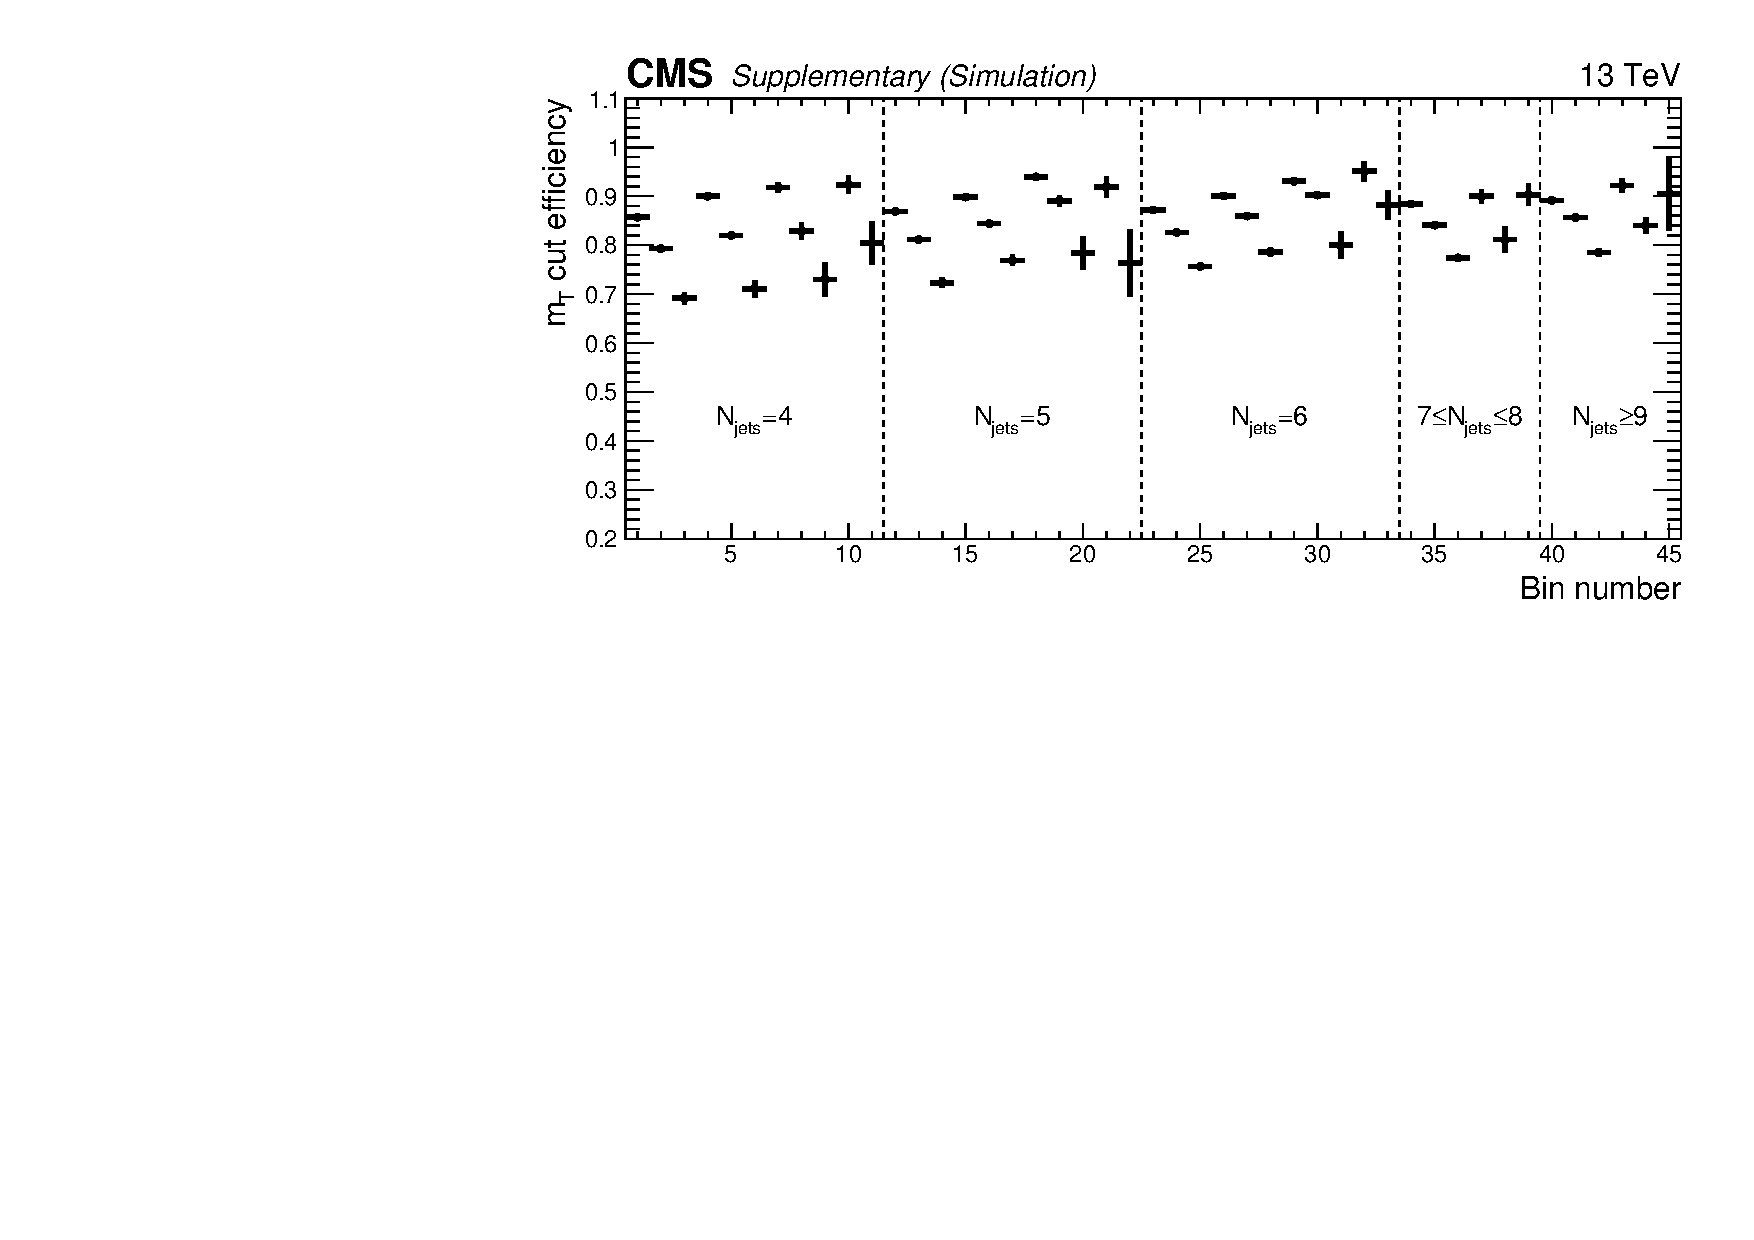
\includegraphics[width=0.9\textwidth]{plot_MtEff.pdf}
  \caption{
    The efficiency $\epsilon_{m_{T}}$ of the muon $m_{T}$ selection. The results are shown as a function of $H_{\rm T}^{\rm miss}$, $H_{\rm T}$, and $N_{\rm jet}$, integrated over the four bins of $N_{\rm b-jet}$ (in total 45 bins).
  }
\end{figure}

\begin{figure}[htb]
  \centering
  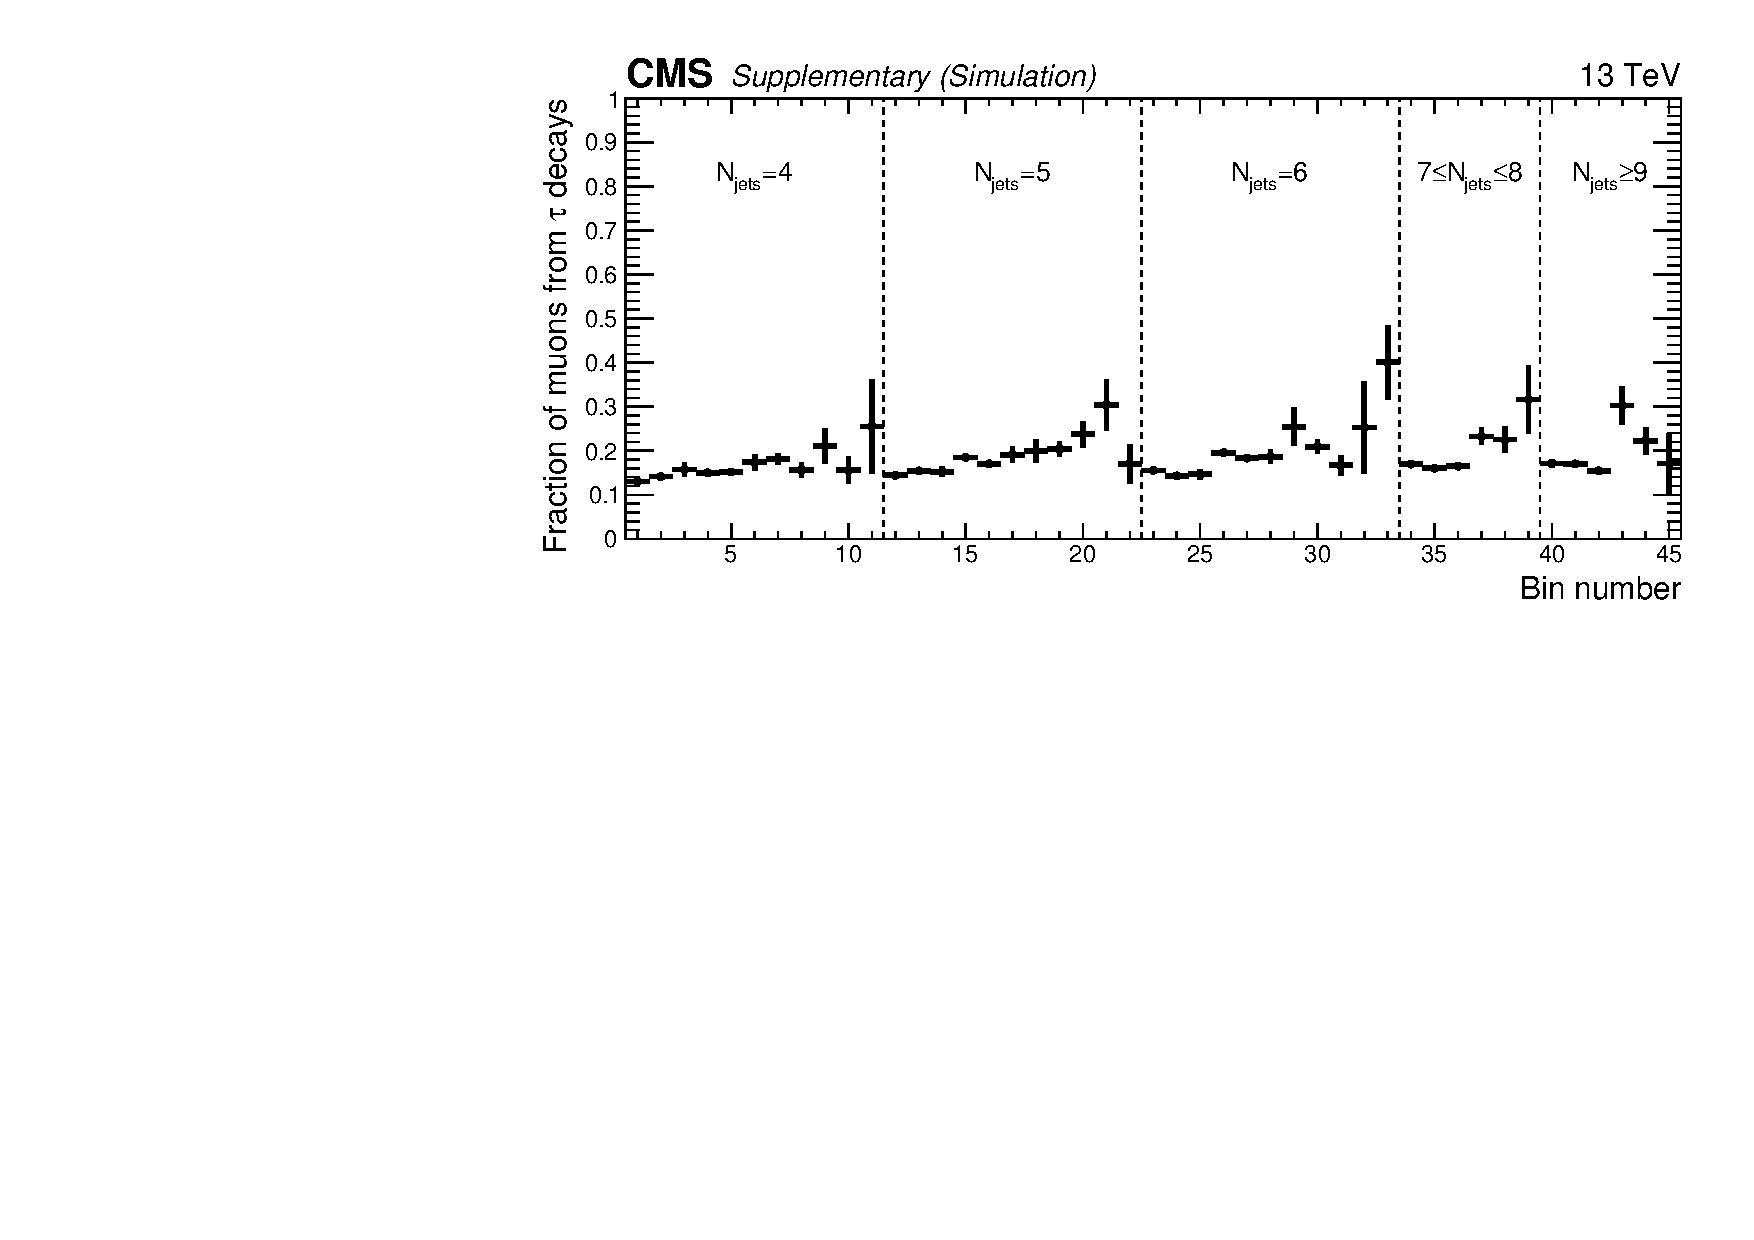
\includegraphics[width=0.9\textwidth]{plot_MuonsFromTaus.pdf}
  \caption{
    The fraction $f $ of muons from $\tau$ decays in the single-muon control sample, as determined from simulation. The results are shown as a function of $H_{\rm T}^{\rm miss}$, $H_{\rm T}$, and $N_{\rm jet}$, integrated over the four bins of $N_{\rm b-jet}$ (in total 45 bins).
  }
\end{figure}

\clearpage


\begin{figure}[h]
  \begin{center}
    \includegraphics[width=0.48\textwidth]{fireworks-258749-361-559467731.png}
  \end{center}
  \caption{
    Event display showing the $\rho-\phi$ plane for event 258749:361:559467731, which has the highest observed $H_{\rm T}^{\rm miss}$ of all events in the search region. Only tracks with $p_{T}>1.5$ GeV are shown.
  }
  \label{fig:evt-display-rho-phi}
\end{figure}


\begin{figure}[h]
  \begin{center}
    \includegraphics[width=0.48\textwidth]{fireworks-258749-361-559467731-white.png}
  \end{center}
  \caption{
    Event display showing the $\rho-\phi$ plane for event 258749:361:559467731, with a white background.
  }
  \label{fig:evt-display-rho-phi-white}
\end{figure}

\clearpage

\begin{figure}[h]
  \begin{center}
    \includegraphics[width=0.48\textwidth]{fireworks-258749-361-559467731-3DTower.png}
  \end{center}
  \caption{
    Event display showing the $\rho-\phi$ plane for event 258749:361:559467731, showing the event in 3D Tower view mode..
  }
  \label{fig:evt-display-rho-phi-3D}
\end{figure}

\begin{figure}[h]
  \begin{center}
    \includegraphics[width=0.48\textwidth]{fireworks-258749-361-559467731-3DTower-light.png}
  \end{center}
  \caption{
    Event display showing the $\rho-\phi$ plane for event 258749:361:559467731, showing the event in 3D Tower view mode with a white background.
  }
  \label{fig:evt-display-rho-phi-3D-white}
\end{figure}

\begin{figure}[htb]
  \begin{center}
    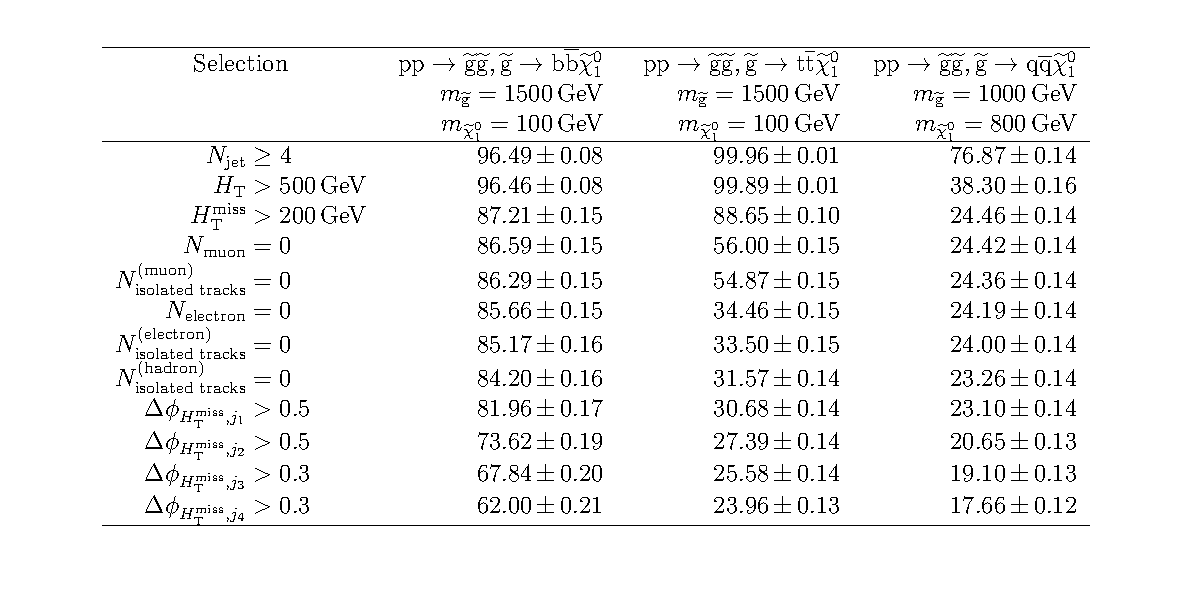
\includegraphics[width=0.9\textwidth]{cutflow2.pdf}
  \end{center}
  \caption{
An expanded and reorganized version of the table of absolute cumulative efficiencies in \% for each step of the event selection process, listed for three representative signal models and choices for the gluino and LSP masses. The lepton and isolated track vetoes are grouped by lepton flavor (muon or electron) and each $\Delta\phi$ cut is shown separately. Only statistical uncertainties are shown. 
  }
  \label{fig:cutflow2}
\end{figure}
\clearpage

\begin{figure}[htb]
\begin{center}
 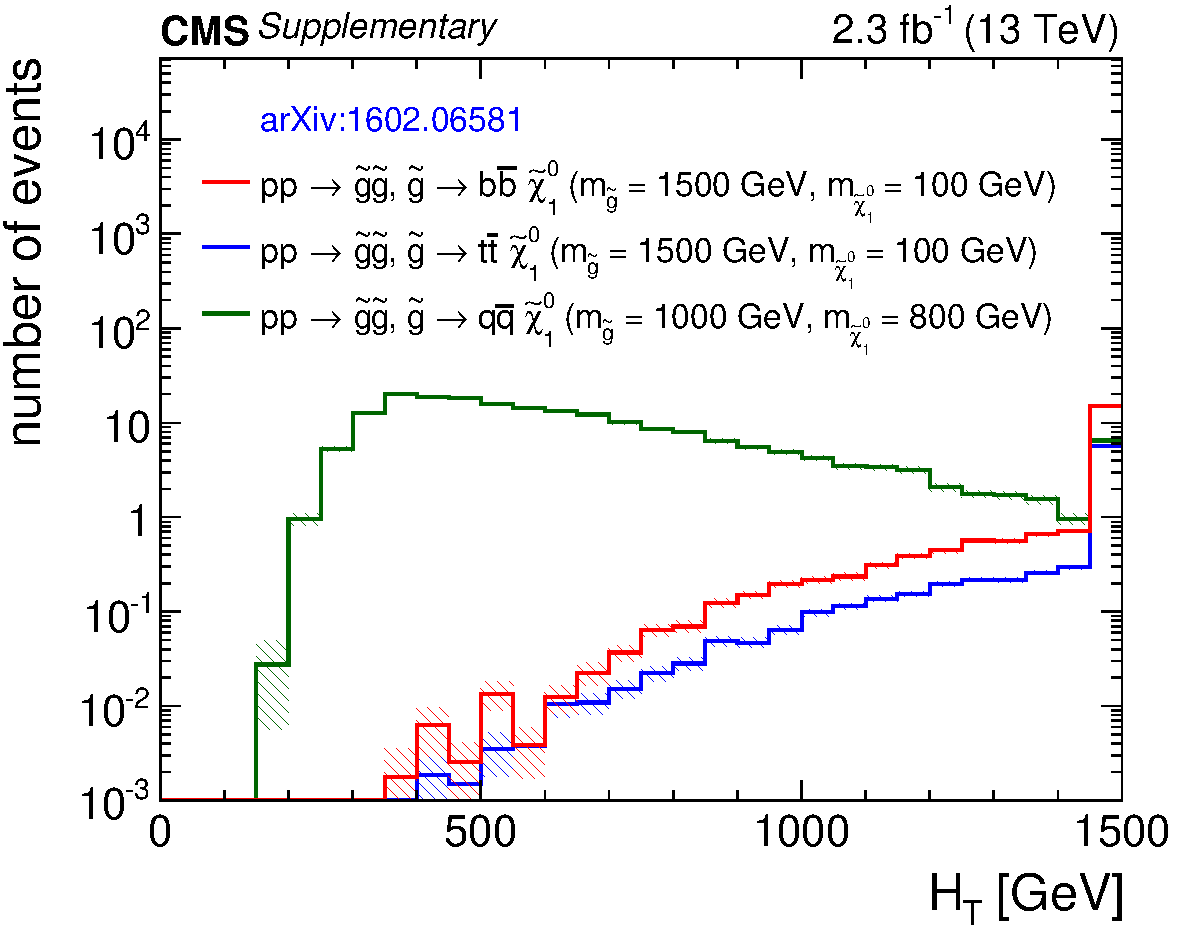
\includegraphics[width=0.48\textwidth]{ht_fast_Nminus1_tree_signalMinusHT.pdf}
 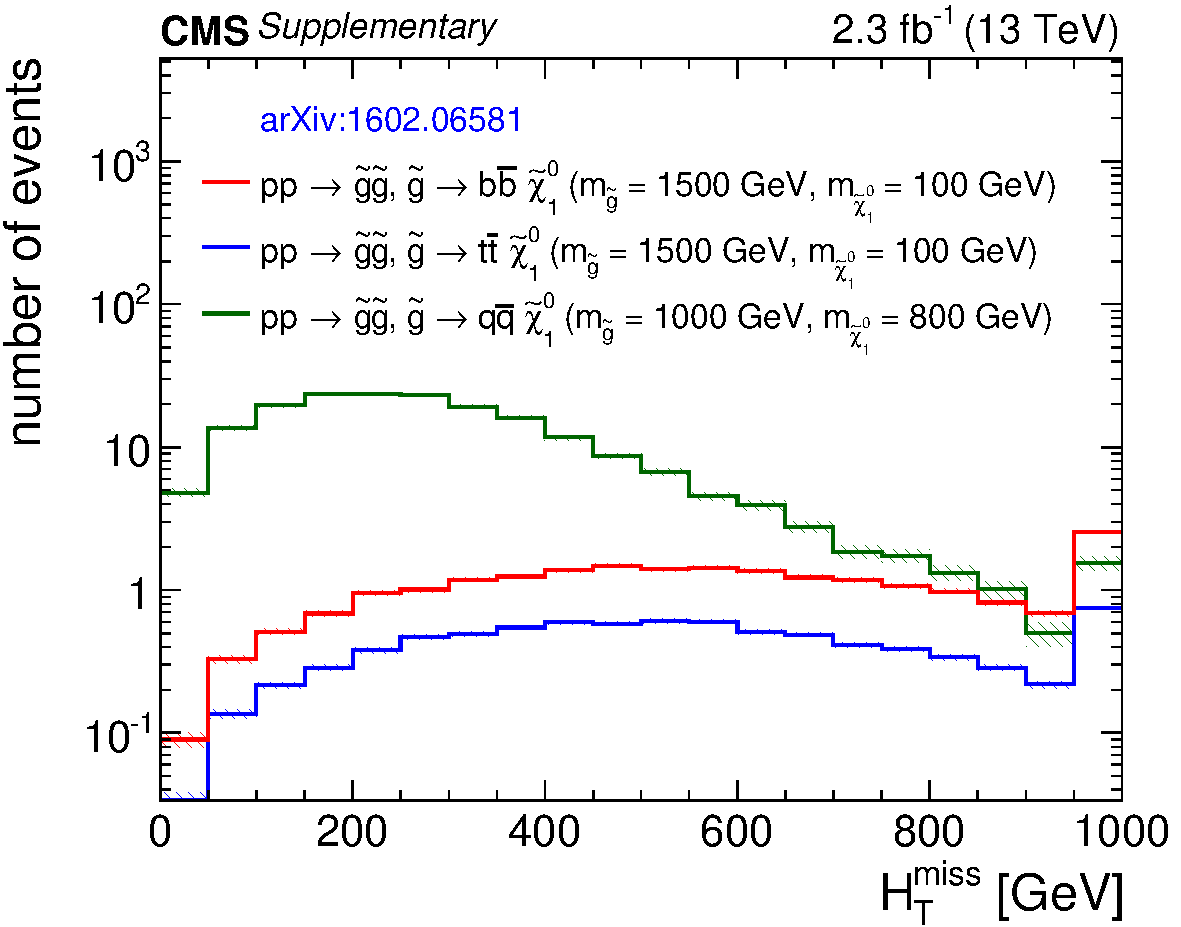
\includegraphics[width=0.48\textwidth]{mht_fast_Nminus1_tree_signalMinusMHT.pdf} \\
  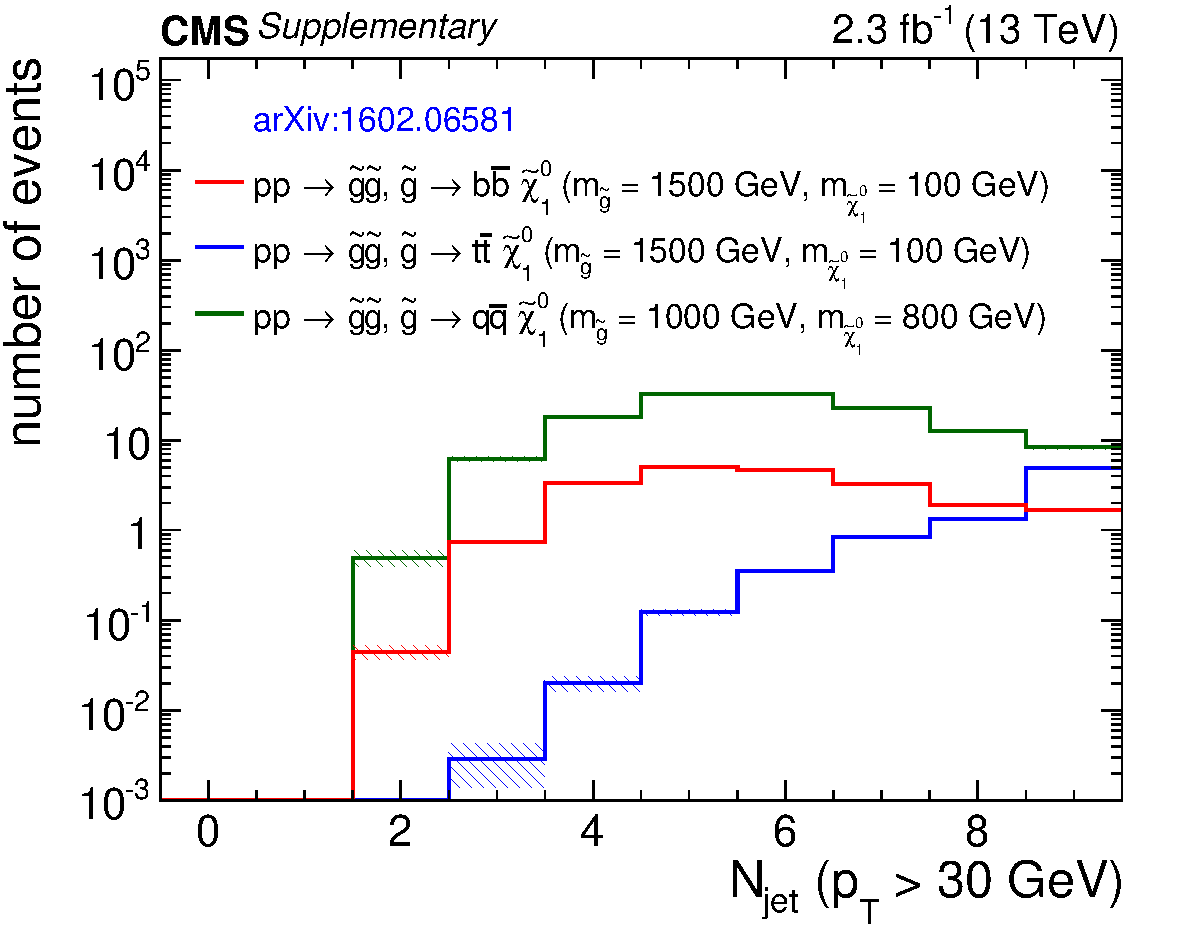
\includegraphics[width=0.48\textwidth]{njets_fast_Nminus1_tree_signalMinusNJet.pdf}
 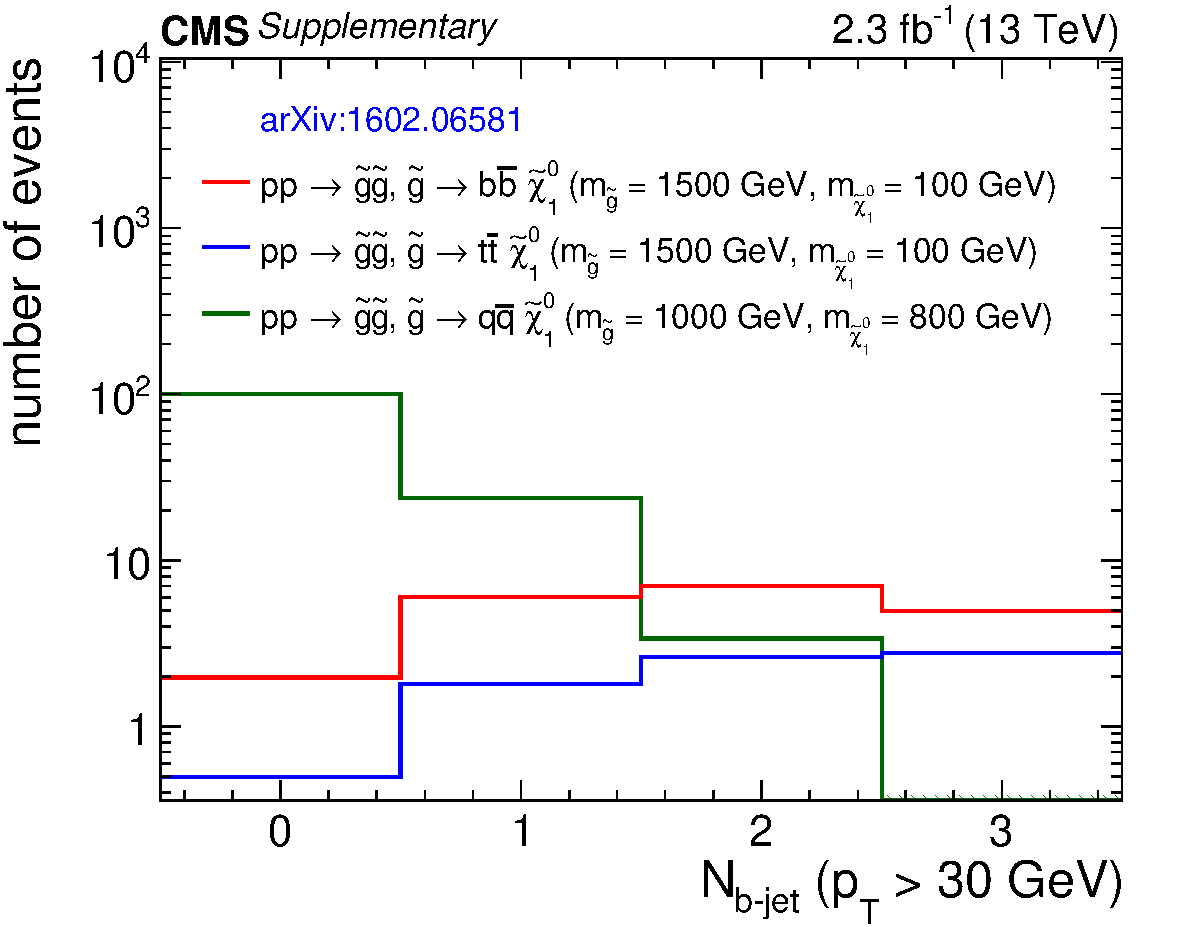
\includegraphics[width=0.48\textwidth]{nbjets_fast_Nminus1_tree_signal.pdf}
  \end{center}
  \caption{
Clockwise from top-left, distributions of $H_{\rm T}$, $H_{\rm T}^{\rm miss}$, the number of b-tagged jets, and the number of jets from three representative signal models after the baseline selection. Each plot ignores the baseline requirement (if any) for its respective variable. The last bin in each plot contains the overflow events. Only statistical uncertainties are shown.
}
\label{fig:fastsim-Nminus1}
\end{figure}
\clearpage

\begin{figure}[htb]
\begin{center}
 \includegraphics[width=0.48\textwidth]{ht_shape_bg_t1qqqq.pdf}
 \includegraphics[width=0.48\textwidth]{mht_shape_bg_t1qqqq.pdf} \\
  \includegraphics[width=0.48\textwidth]{njets_shape_bg_t1tttt.pdf}
 \includegraphics[width=0.48\textwidth]{nbjets_shape_bg_t1bbbb.pdf}
  \end{center}
  \caption{
Clockwise from top-left, kinematic shape comparisons showing distributions of $H_{\rm T}$, $H_{\rm T}^{\rm miss}$, the number of b-tagged jets, and the number of jets for the main background processes and six example gluino production signal models. The full baseline selection is applied in each plot.
}
\label{fig:bg-sig-shapes}
\end{figure}
\clearpage

\begin{figure}[htb]
\begin{center}
 \includegraphics[width=0.48\textwidth]{SMSbbbbSigEff.pdf}
 \includegraphics[width=0.48\textwidth]{SMSttttSigEff.pdf} \\
  \includegraphics[width=0.48\textwidth]{SMSqqqqSigEff.pdf}
 \includegraphics[width=0.48\textwidth]{SMSqqqqVVSigEff.pdf}
  \end{center}
  \caption{
The product of signal efficiency and acceptance for the baseline selection in the $m_{\tilde{\chi}_{1}^{0}}-m_{\tilde{\rm g}}$ mass plane. Clockwise from top-left are the SMS models T1bbbb, T1tttt, T5qqqqVV, T1qqqq.
}
\label{fig:SMSsigEff}
\end{figure}
\clearpage

\begin{figure}[h]
  \begin{center}
    \includegraphics[width=0.98\textwidth]{t1-signal-q-plot-72-bins.pdf}
  \end{center}
  \caption{
    The sensitivity of the analysis to different direct gluino production signal models as a function of the analysis binning. The upper panel shows the total predicted SM backgrounds and the expected number of signal events for six representative model points per analysis bin. The bottom panel shows the expected sensitivity, expressed in terms of the figure of merit Q, per analysis bin.
  }
  \label{fig:t1-q-plot}
\end{figure}

\begin{figure}[h]
  \begin{center}
    \includegraphics[width=0.98\textwidth]{t2-signal-q-plot-72-bins.pdf}
  \end{center}
  \caption{
    The sensitivity of the analysis to different direct squark production signal models as a function of the analysis binning. The upper panel shows the total predicted SM backgrounds and the expected number of signal events for six representative model points per analysis bin. The bottom panel shows the expected sensitivity, expressed in terms of the figure of merit Q, per analysis bin.
  }
  \label{fig:t2-q-plot}
\end{figure}



\begin{figure}[h]
  \begin{center}
    \includegraphics[width=0.98\textwidth]{ZgammaRatioWOSF.pdf}
  \end{center}
  \caption{
    The $\rm{Z}(\nu\nu)/\gamma$ ratio calculated using leading order Monte Carlo simulation in the search bins with $N_{\rm{b-jet}}=0$.
  }
  \label{fig:ZgammaRatio-plot}
\end{figure}


\begin{figure}[h]
  \begin{center}
    \includegraphics[width=0.98\textwidth]{ZgR_vs_HT.pdf}
  \end{center}
  \caption{
    The $\rm{Z}(\nu\nu)/\gamma$ ratio vs. $H_{\rm{T}}$ calculated using leading order Monte Carlo simulation.
  }
  \label{fig:ZgammaRatioVsHT-plot}
\end{figure}


\begin{figure}[h]
  \begin{center}
    \includegraphics[width=0.98\textwidth]{ZgR_vs_MHT.pdf}
  \end{center}
  \caption{
    The $\rm{Z}(\nu\nu)/\gamma$ ratio vs. $H_{\rm{T}}^{\rm{miss}}$ calculated using leading order Monte Carlo simulation.
  }
  \label{fig:ZgammaRatioVsMHT-plot}
\end{figure}



\begin{figure}[h]
  \begin{center}
    \includegraphics[width=0.98\textwidth]{ZgR_vs_NJets.pdf}
  \end{center}
  \caption{
    The $\rm{Z}(\nu\nu)/\gamma$ ratio vs. $N_{\rm{jet}}$ calculated using leading order Monte Carlo simulation.
  }
  \label{fig:ZgammaRatioVsNJets-plot}
\end{figure}

\begin{figure}[h]
  \begin{center}
    \includegraphics[width=0.98\textwidth]{poststack_log.pdf}
  \end{center}
  \caption{
    Observed numbers of events and corresponding SM background predictions in the 72 search regions of the analysis after the final fit performed with the assumption of only standard model contributions. Background predictions before the final fit are also shown for comparison. The lower panel shows the pull distributions for the data and the pre-fit background estimates with respect to the post-fit background estimates.
  }
  \label{fig:poststack_log}
\end{figure}


\newcolumntype{R}{>{$}r<{$}}
\newcolumntype{L}{>{$}l<{$}}
\newcolumntype{M}{L@{$\;$}L}
\newcolumntype{S}{r@{$\,\pm\,$}r}
\begin{table*}[htb]
\caption{Expected numbers of events in search bins with $4\leq\njets\leq6$ for three representative signal models. Only statistical uncertainties are shown.}
\centering
    \begin{tabular}{cccc|ccc}
\hline
&&&& $\Pp\Pp \to \PSg\PSg, \PSg \to \bbbar \PSGczDo$ &$\Pp\Pp \to \PSg\PSg, \PSg \to \ttbar \PSGczDo$ &$\Pp\Pp \to \PSg\PSg, \PSg \to \qqbar \PSGczDo$ \\
Bin & $H_{\rm T}^{\rm miss}$ [GeV] & $H_{\rm T}$ [GeV] & $\nbjets$ & $m_{\PSg}=1500$ GeV & $m_{\PSg}=1500$ GeV & $m_{\PSg}=1000$ GeV \\
&&&& $m_{\PSGczDo}=100$ GeV  &$m_{\PSGczDo}=100$ GeV &$m_{\PSGczDo}=800$ GeV \\
%\multicolumn{2}{c}{}          &$m_{\PSg}=1500$ GeV}                                       &$m_{\PSg}=1500$ GeV}                                       &$m_{\PSg}=1000$ GeV} \\
%\multicolumn{2}{c}{}          &                            $m_{\PSGczDo}=100$ GeV}                                    &$m_{\PSGczDo}=100$ GeV}                                    &$m_{\PSGczDo}=800$ GeV} \\
\hline
1 & 200-500 & 500-800 & 0 & $0.01 \pm 0.00$ & $0.00 \pm 0.00$ & $58.45 \pm 1.09$ \\
2 & 200-500 & 800-1200 & 0 & $0.05 \pm 0.00$ & $0.00 \pm 0.00$ & $13.30 \pm 0.51$ \\
3 & 200-500 & 1200+ & 0 & $0.63 \pm 0.02$ & $0.03 \pm 0.00$ & $1.36 \pm 0.16$ \\
4 & 500-750 & 500-1200 & 0 & $0.05 \pm 0.00$ & $0.01 \pm 0.00$ & $10.80 \pm 0.50$ \\
5 & 500-750 & 1200+ & 0 & $0.55 \pm 0.01$ & $0.03 \pm 0.00$ & $2.13 \pm 0.21$ \\
6 & 750+ & 800+ & 0 & $0.58 \pm 0.01$ & $0.03 \pm 0.00$ & $3.48 \pm 0.27$ \\
7 & 200-500 & 500-800 & 1 & $0.03 \pm 0.00$ & $0.01 \pm 0.00$ & $11.60 \pm 0.27$ \\
8 & 200-500 & 800-1200 & 1 & $0.19 \pm 0.01$ & $0.01 \pm 0.00$ & $3.15 \pm 0.14$ \\
9 & 200-500 & 1200+ & 1 & $1.73 \pm 0.04$ & $0.06 \pm 0.00$ & $0.27 \pm 0.04$ \\
10 & 500-750 & 500-1200 & 1 & $0.20 \pm 0.01$ & $0.02 \pm 0.00$ & $2.25 \pm 0.12$ \\
11 & 500-750 & 1200+ & 1 & $1.58 \pm 0.03$ & $0.06 \pm 0.01$ & $0.43 \pm 0.05$ \\
12 & 750+ & 800+ & 1 & $1.73 \pm 0.03$ & $0.07 \pm 0.01$ & $0.58 \pm 0.06$ \\
13 & 200-500 & 500-800 & 2 & $0.04 \pm 0.01$ & $0.01 \pm 0.00$ & $1.26 \pm 0.05$ \\
14 & 200-500 & 800-1200 & 2 & $0.29 \pm 0.01$ & $0.01 \pm 0.00$ & $0.38 \pm 0.03$ \\
15 & 200-500 & 1200+ & 2 & $1.79 \pm 0.04$ & $0.05 \pm 0.00$ & $0.03 \pm 0.01$ \\
16 & 500-750 & 500-1200 & 2 & $0.29 \pm 0.02$ & $0.02 \pm 0.00$ & $0.27 \pm 0.03$ \\
17 & 500-750 & 1200+ & 2 & $1.72 \pm 0.03$ & $0.05 \pm 0.00$ & $0.04 \pm 0.01$ \\
18 & 750+ & 800+ & 2 & $1.89 \pm 0.04$ & $0.06 \pm 0.00$ & $0.05 \pm 0.01$ \\
19 & 200-500 & 500-800 & 3+ & $0.03 \pm 0.01$ & $0.00 \pm 0.00$ & $0.08 \pm 0.01$ \\
20 & 200-500 & 800-1200 & 3+ & $0.25 \pm 0.01$ & $0.01 \pm 0.00$ & $0.04 \pm 0.01$ \\
21 & 200-500 & 1200+ & 3+ & $1.06 \pm 0.03$ & $0.02 \pm 0.00$ & $0.00 \pm 0.00$ \\
22 & 500-750 & 500-1200 & 3+ & $0.25 \pm 0.02$ & $0.01 \pm 0.00$ & $0.02 \pm 0.00$ \\
23 & 500-750 & 1200+ & 3+ & $1.04 \pm 0.03$ & $0.03 \pm 0.00$ & $0.00 \pm 0.00$ \\
24 & 750+ & 800+ & 3+ & $1.10 \pm 0.03$ & $0.03 \pm 0.00$ & $0.00 \pm 0.00$ \\ \hline
\hline
\end{tabular}
  \label{tab:sig-bins-1}
\end{table*}

\begin{table*}[htb]
\caption{Expected numbers of events in search bins with $7\leq\njets\leq8$ for three representative signal models. Only statistical uncertainties are shown.}
\centering
    \begin{tabular}{cccc|ccc}
\hline
&&&& $\Pp\Pp \to \PSg\PSg, \PSg \to \bbbar \PSGczDo$ &$\Pp\Pp \to \PSg\PSg, \PSg \to \ttbar \PSGczDo$ &$\Pp\Pp \to \PSg\PSg, \PSg \to \qqbar \PSGczDo$ \\
Bin & $H_{\rm T}^{\rm miss}$ [GeV] & $H_{\rm T}$ [GeV] & $\nbjets$ & $m_{\PSg}=1500$ GeV & $m_{\PSg}=1500$ GeV & $m_{\PSg}=1000$ GeV \\
&&&& $m_{\PSGczDo}=100$ GeV  &$m_{\PSGczDo}=100$ GeV &$m_{\PSGczDo}=800$ GeV \\
%\multicolumn{2}{c}{}          &$m_{\PSg}=1500$ GeV}                                       &$m_{\PSg}=1500$ GeV}                                       &$m_{\PSg}=1000$ GeV} \\
%\multicolumn{2}{c}{}          &                            $m_{\PSGczDo}=100$ GeV}                                    &$m_{\PSGczDo}=100$ GeV}                                    &$m_{\PSGczDo}=800$ GeV} \\
\hline
25 & 200-500 & 500-800 & 0 & $0.00 \pm 0.00$ & $0.00 \pm 0.00$ & $14.25 \pm 0.52$ \\
26 & 200-500 & 800-1200 & 0 & $0.01 \pm 0.00$ & $0.01 \pm 0.00$ & $10.67 \pm 0.46$ \\
27 & 200-500 & 1200+ & 0 & $0.20 \pm 0.01$ & $0.08 \pm 0.00$ & $2.37 \pm 0.21$ \\
28 & 500-750 & 500-1200 & 0 & $0.00 \pm 0.00$ & $0.01 \pm 0.00$ & $3.68 \pm 0.27$ \\
29 & 500-750 & 1200+ & 0 & $0.17 \pm 0.01$ & $0.07 \pm 0.00$ & $1.86 \pm 0.19$ \\
30 & 750+ & 800+ & 0 & $0.17 \pm 0.01$ & $0.06 \pm 0.00$ & $1.92 \pm 0.19$ \\
31 & 200-500 & 500-800 & 1 & $0.00 \pm 0.00$ & $0.01 \pm 0.00$ & $3.80 \pm 0.17$ \\
32 & 200-500 & 800-1200 & 1 & $0.03 \pm 0.00$ & $0.04 \pm 0.00$ & $2.96 \pm 0.15$ \\
33 & 200-500 & 1200+ & 1 & $0.65 \pm 0.02$ & $0.26 \pm 0.01$ & $0.70 \pm 0.07$ \\
34 & 500-750 & 500-1200 & 1 & $0.02 \pm 0.00$ & $0.04 \pm 0.00$ & $1.13 \pm 0.09$ \\
35 & 500-750 & 1200+ & 1 & $0.58 \pm 0.02$ & $0.21 \pm 0.01$ & $0.57 \pm 0.06$ \\
36 & 750+ & 800+ & 1 & $0.58 \pm 0.02$ & $0.22 \pm 0.01$ & $0.45 \pm 0.05$ \\
37 & 200-500 & 500-800 & 2 & $0.00 \pm 0.00$ & $0.01 \pm 0.00$ & $0.62 \pm 0.05$ \\
38 & 200-500 & 800-1200 & 2 & $0.05 \pm 0.01$ & $0.06 \pm 0.00$ & $0.49 \pm 0.04$ \\
39 & 200-500 & 1200+ & 2 & $0.81 \pm 0.02$ & $0.32 \pm 0.01$ & $0.16 \pm 0.03$ \\
40 & 500-750 & 500-1200 & 2 & $0.04 \pm 0.00$ & $0.06 \pm 0.00$ & $0.19 \pm 0.03$ \\
41 & 500-750 & 1200+ & 2 & $0.74 \pm 0.02$ & $0.26 \pm 0.01$ & $0.11 \pm 0.02$ \\
42 & 750+ & 800+ & 2 & $0.74 \pm 0.02$ & $0.28 \pm 0.01$ & $0.07 \pm 0.01$ \\
43 & 200-500 & 500-800 & 3+ & $0.00 \pm 0.00$ & $0.01 \pm 0.00$ & $0.08 \pm 0.02$ \\
44 & 200-500 & 800-1200 & 3+ & $0.06 \pm 0.01$ & $0.06 \pm 0.00$ & $0.05 \pm 0.01$ \\
45 & 200-500 & 1200+ & 3+ & $0.65 \pm 0.02$ & $0.26 \pm 0.01$ & $0.03 \pm 0.01$ \\
46 & 500-750 & 500-1200 & 3+ & $0.04 \pm 0.01$ & $0.06 \pm 0.00$ & $0.02 \pm 0.00$ \\
47 & 500-750 & 1200+ & 3+ & $0.59 \pm 0.02$ & $0.20 \pm 0.01$ & $0.02 \pm 0.01$ \\
48 & 750+ & 800+ & 3+ & $0.57 \pm 0.02$ & $0.22 \pm 0.01$ & $0.01 \pm 0.00$ \\
\hline
\end{tabular}
  \label{tab:sig-bins-2}
\end{table*}

\begin{table*}[htb]
\caption{Expected numbers of events in search bins with $\njets\geq9$ for three representative signal models. Only statistical uncertainties are shown.}
\centering
    \begin{tabular}{cccc|ccc}
\hline
&&&& $\Pp\Pp \to \PSg\PSg, \PSg \to \bbbar \PSGczDo$ &$\Pp\Pp \to \PSg\PSg, \PSg \to \ttbar \PSGczDo$ &$\Pp\Pp \to \PSg\PSg, \PSg \to \qqbar \PSGczDo$ \\
Bin & $H_{\rm T}^{\rm miss}$ [GeV] & $H_{\rm T}$ [GeV] & $\nbjets$ & $m_{\PSg}=1500$ GeV & $m_{\PSg}=1500$ GeV & $m_{\PSg}=1000$ GeV \\
&&&& $m_{\PSGczDo}=100$ GeV  &$m_{\PSGczDo}=100$ GeV &$m_{\PSGczDo}=800$ GeV \\
%\multicolumn{2}{c}{}          &$m_{\PSg}=1500$ GeV}                                       &$m_{\PSg}=1500$ GeV}                                       &$m_{\PSg}=1000$ GeV} \\
%\multicolumn{2}{c}{}          &                            $m_{\PSGczDo}=100$ GeV}                                    &$m_{\PSGczDo}=100$ GeV}                                    &$m_{\PSGczDo}=800$ GeV} \\
\hline
49 & 200-500 & 500-800 & 0 & $0.00 \pm 0.00$ & $0.00 \pm 0.00$ & $1.16 \pm 0.14$ \\
50 & 200-500 & 800-1200 & 0 & $0.00 \pm 0.00$ & $0.01 \pm 0.00$ & $2.64 \pm 0.22$ \\
51 & 200-500 & 1200+ & 0 & $0.06 \pm 0.00$ & $0.12 \pm 0.00$ & $1.06 \pm 0.13$ \\
52 & 500-750 & 500-1200 & 0 & $0.00 \pm 0.00$ & $0.01 \pm 0.00$ & $0.64 \pm 0.11$ \\
53 & 500-750 & 1200+ & 0 & $0.05 \pm 0.00$ & $0.10 \pm 0.00$ & $0.88 \pm 0.12$ \\
54 & 750+ & 800+ & 0 & $0.04 \pm 0.00$ & $0.08 \pm 0.00$ & $0.85 \pm 0.12$ \\
55 & 200-500 & 500-800 & 1 & $0.00 \pm 0.00$ & $0.00 \pm 0.00$ & $0.38 \pm 0.05$ \\
56 & 200-500 & 800-1200 & 1 & $0.00 \pm 0.00$ & $0.04 \pm 0.00$ & $1.08 \pm 0.10$ \\
57 & 200-500 & 1200+ & 1 & $0.20 \pm 0.01$ & $0.49 \pm 0.01$ & $0.44 \pm 0.06$ \\
58 & 500-750 & 500-1200 & 1 & $0.00 \pm 0.00$ & $0.03 \pm 0.00$ & $0.22 \pm 0.04$ \\
59 & 500-750 & 1200+ & 1 & $0.18 \pm 0.01$ & $0.42 \pm 0.01$ & $0.36 \pm 0.05$ \\
60 & 750+ & 800+ & 1 & $0.15 \pm 0.01$ & $0.34 \pm 0.01$ & $0.37 \pm 0.06$ \\
61 & 200-500 & 500-800 & 2 & $0.00 \pm 0.00$ & $0.00 \pm 0.00$ & $0.07 \pm 0.01$ \\
62 & 200-500 & 800-1200 & 2 & $0.01 \pm 0.00$ & $0.07 \pm 0.00$ & $0.26 \pm 0.04$ \\
63 & 200-500 & 1200+ & 2 & $0.29 \pm 0.01$ & $0.81 \pm 0.02$ & $0.12 \pm 0.03$ \\
64 & 500-750 & 500-1200 & 2 & $0.00 \pm 0.00$ & $0.05 \pm 0.00$ & $0.04 \pm 0.01$ \\
65 & 500-750 & 1200+ & 2 & $0.25 \pm 0.01$ & $0.71 \pm 0.02$ & $0.10 \pm 0.02$ \\
66 & 750+ & 800+ & 2 & $0.21 \pm 0.01$ & $0.54 \pm 0.01$ & $0.12 \pm 0.03$ \\
67 & 200-500 & 500-800 & 3+ & $0.00 \pm 0.00$ & $0.01 \pm 0.00$ & $0.01 \pm 0.00$ \\
68 & 200-500 & 800-1200 & 3+ & $0.01 \pm 0.00$ & $0.08 \pm 0.01$ & $0.05 \pm 0.01$ \\
69 & 200-500 & 1200+ & 3+ & $0.29 \pm 0.02$ & $1.02 \pm 0.02$ & $0.02 \pm 0.01$ \\
70 & 500-750 & 500-1200 & 3+ & $0.00 \pm 0.00$ & $0.06 \pm 0.00$ & $0.00 \pm 0.00$ \\
71 & 500-750 & 1200+ & 3+ & $0.26 \pm 0.01$ & $0.89 \pm 0.02$ & $0.02 \pm 0.01$ \\
72 & 750+ & 800+ & 3+ & $0.21 \pm 0.01$ & $0.65 \pm 0.02$ & $0.02 \pm 0.01$ \\
\hline
\end{tabular}
  \label{tab:sig-bins-2}
\end{table*}




\end{document}  
